%% The "\appendix" call has already been made in the declaration
%% of the "appendices" environment (see thesis.tex).
\chapter{Shape systematics}
\label{app:shape}

In the binned likelihood fit, systematics are taken into account in the form of nuisance parameters. In cases where the nuisance parameter can affect the \ptmiss shape and normalization of a given signal or background process, it is necessary to construct the \ptmiss shape after the $\pm 1\sigma$ uncertainty variation is propagated to this observable. The relevant shape systematics are detailed in \SectionRef{subsec:sources}, and are shown for the dominant background, SM \ttll in \SectionRef{sec:tt2lsyst} and for a scalar mediated signal with $\mMed=10\:\GeV$ and $\mDM=1\:\GeV$ in \SectionRef{sec:s10syst}.

\clearpage

\section{\ttll shape systematics}
\label{sec:tt2lsyst}

\begin{figure}[h]
  \centering
  \subfloat[][\ttll, low \mttll-SF]{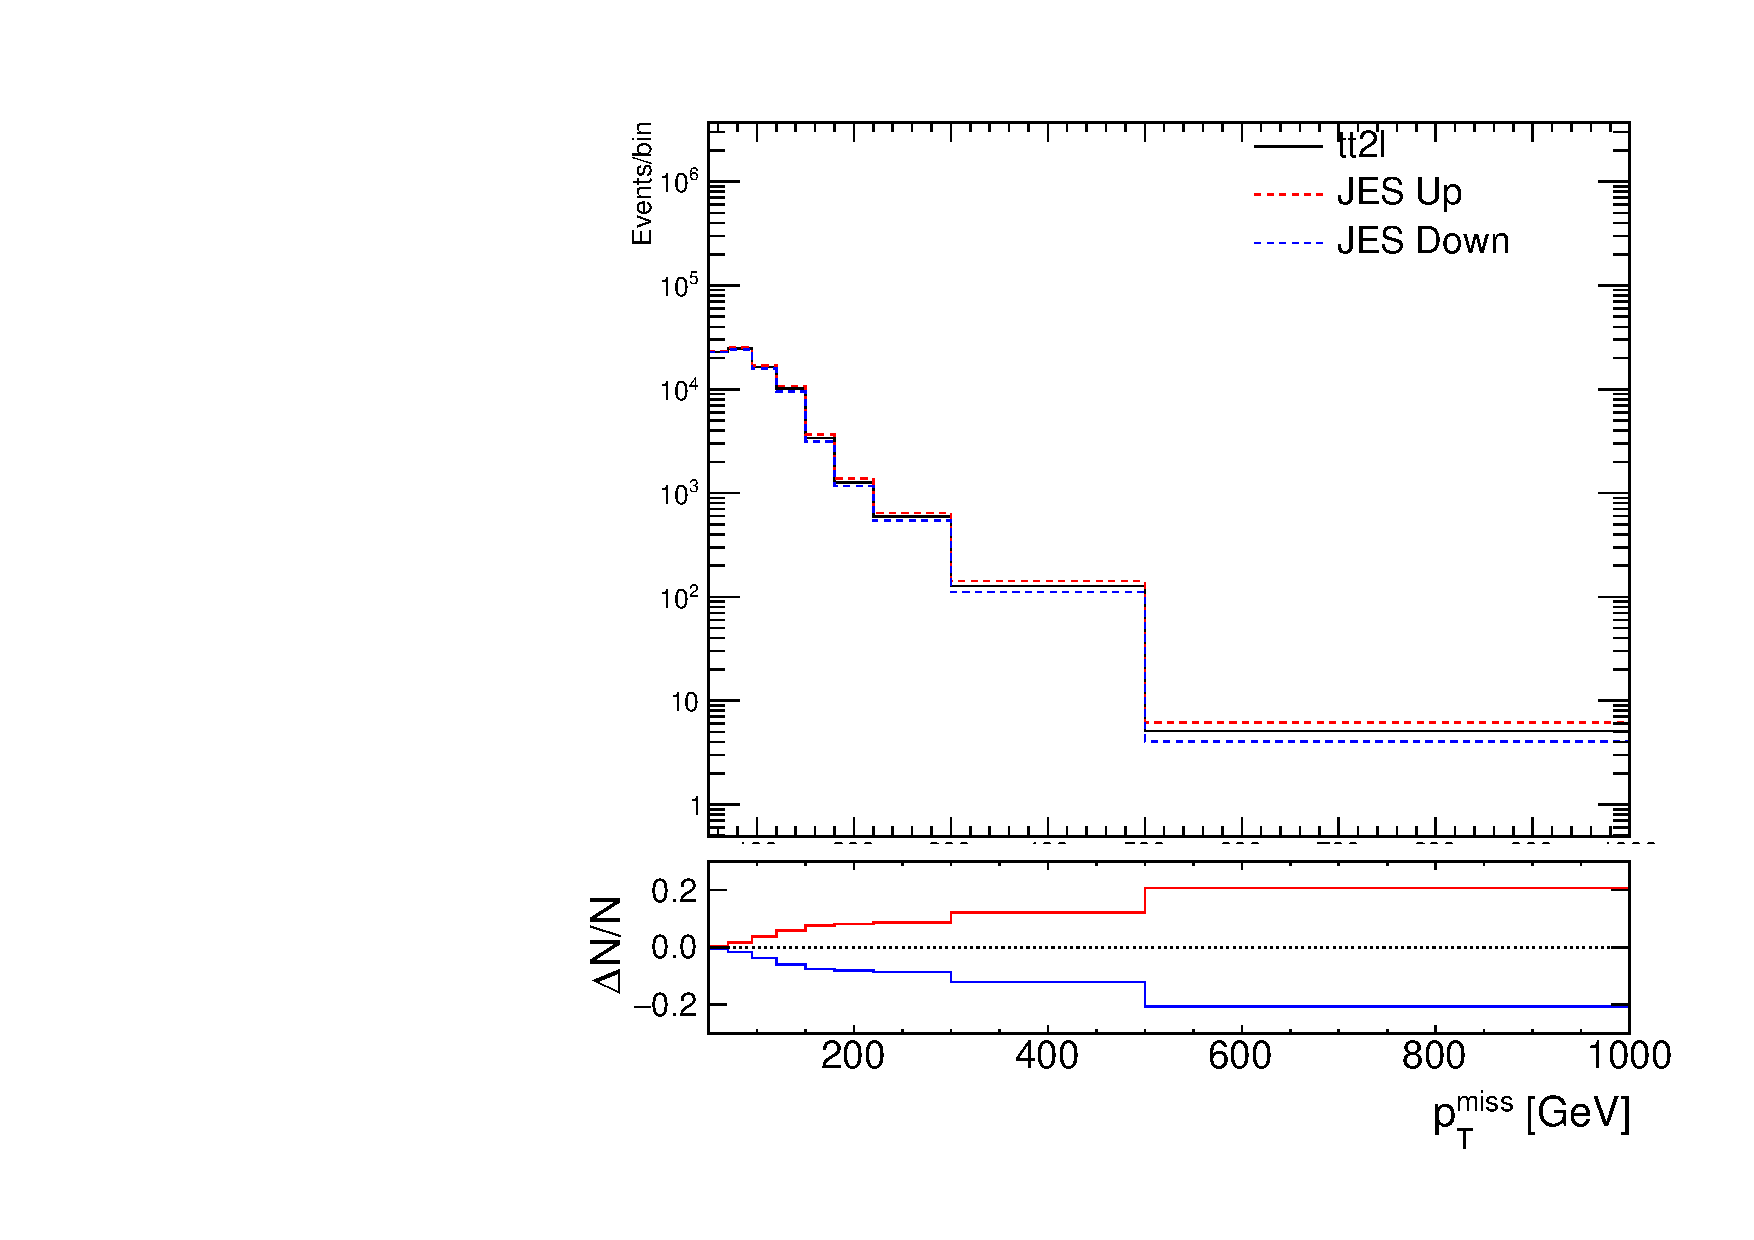
\includegraphics[width=0.48\textwidth]{systs/shapes_ttdm805101_sf_lo/tt2l_CMS_scale_j}}
  \subfloat[][\ttll, low \mttll-OF]{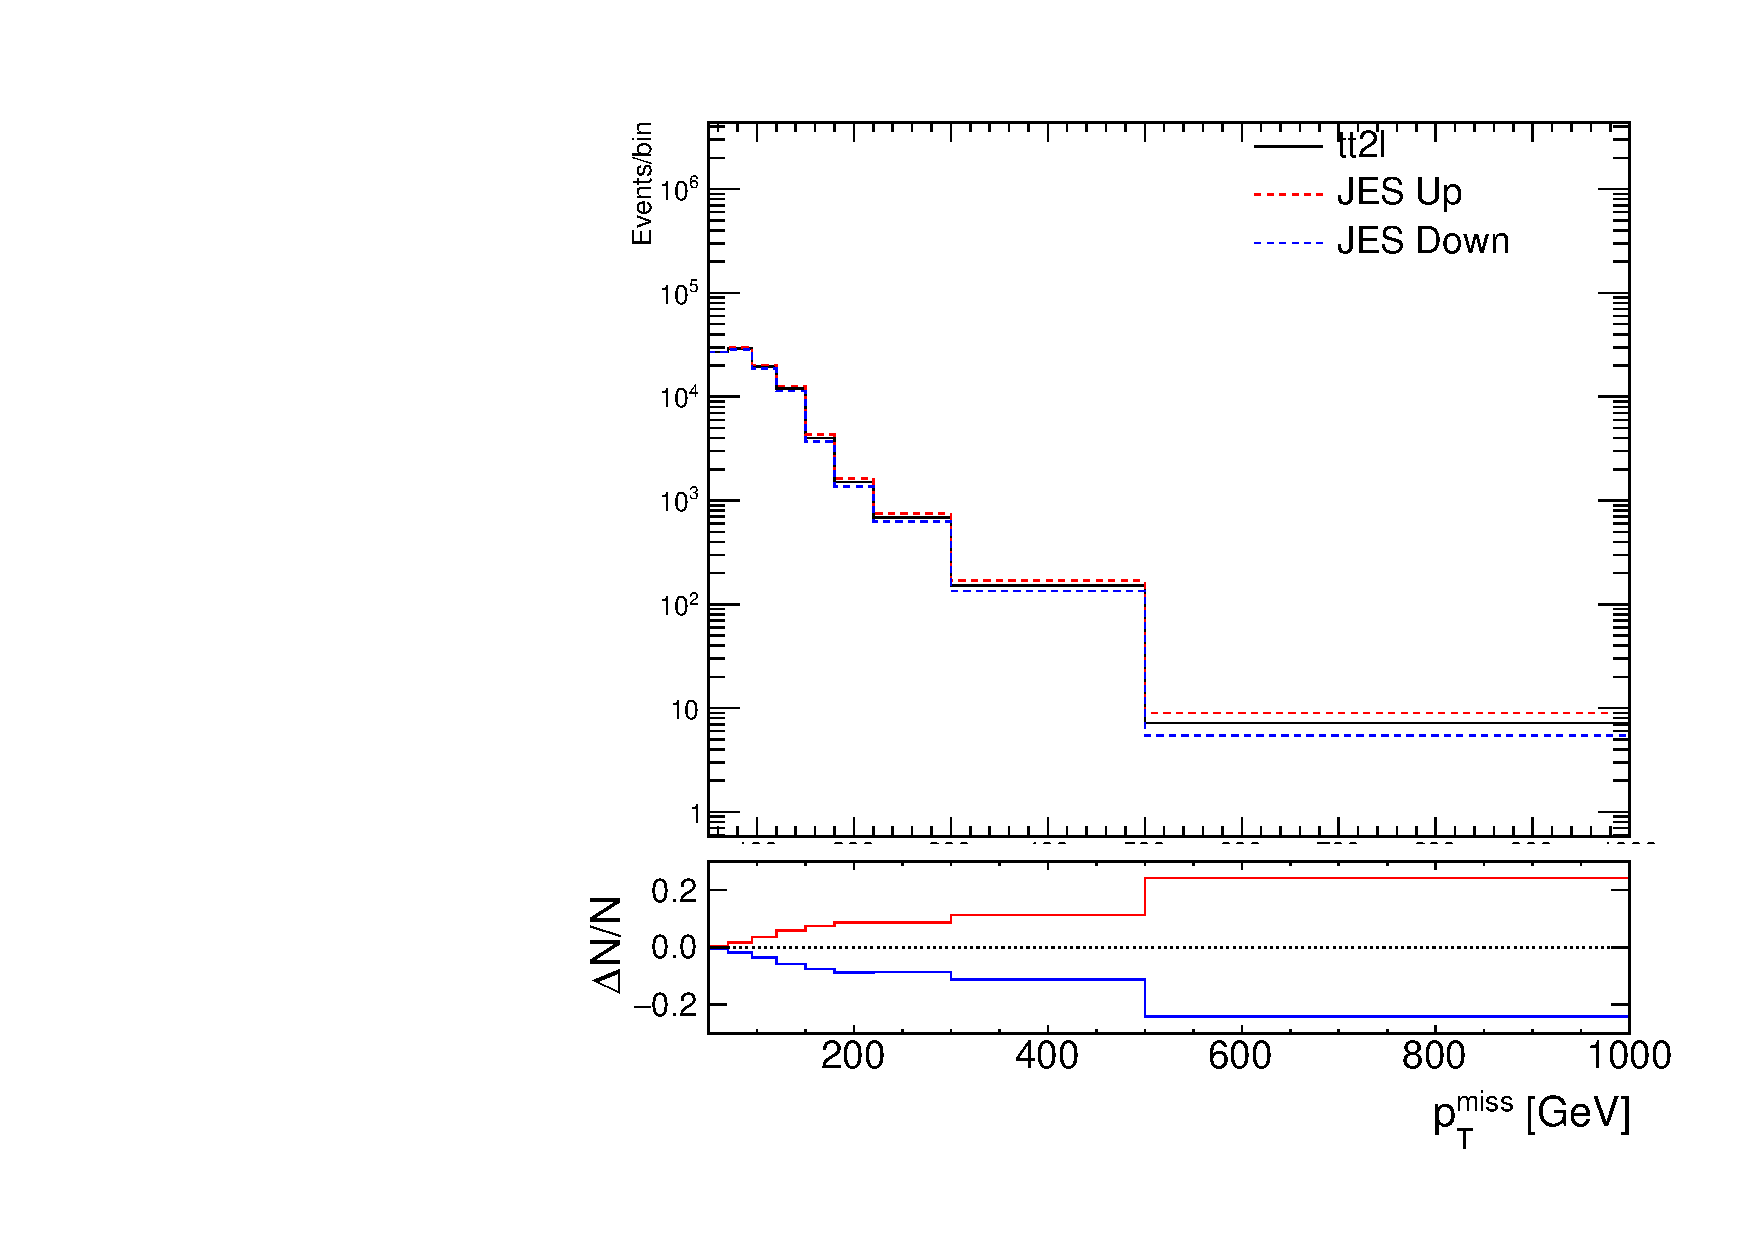
\includegraphics[width=0.48\textwidth]{systs/shapes_ttdm805101_em_lo/tt2l_CMS_scale_j}} \\
  \subfloat[][\ttll, high \mttll-SF]{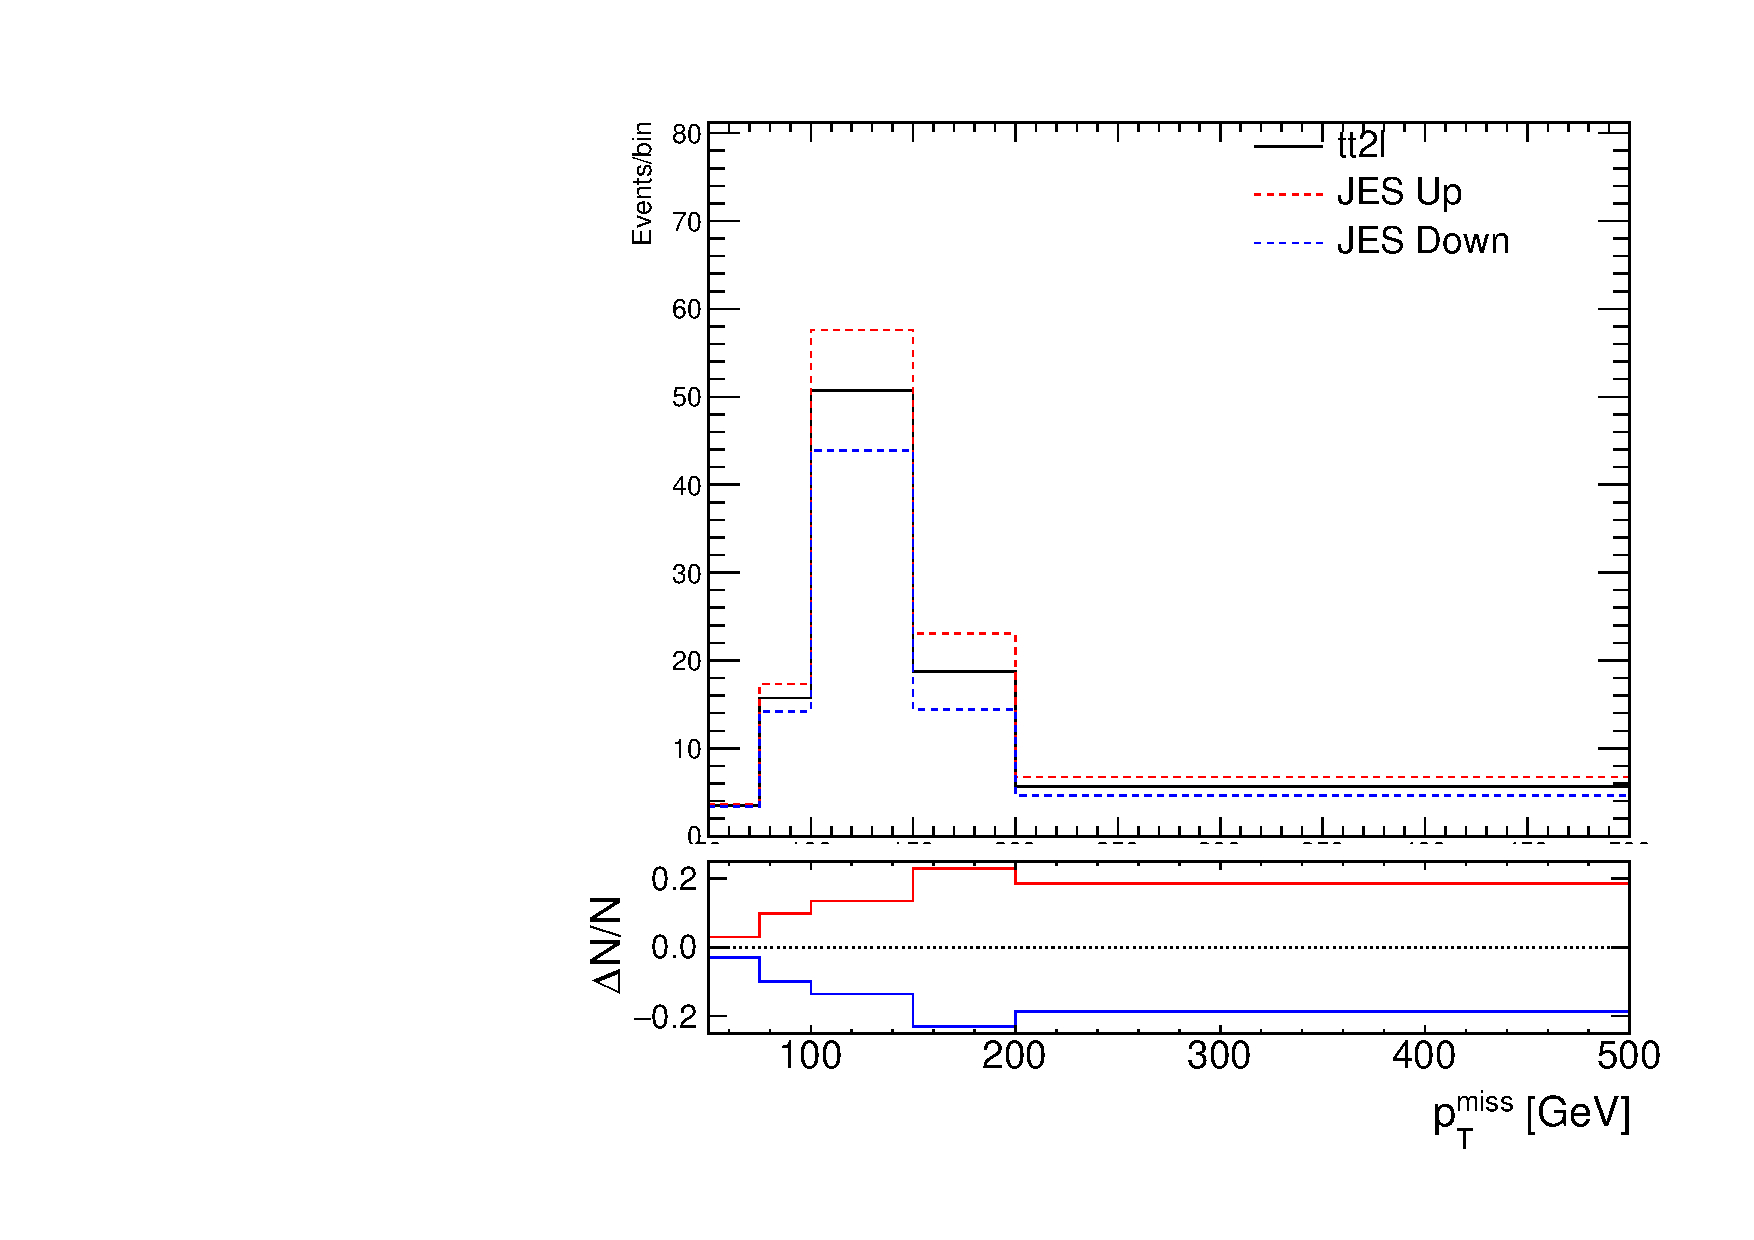
\includegraphics[width=0.48\textwidth]{systs/shapes_ttdm805101_sf_hi/tt2l_CMS_scale_j}}
  \subfloat[][\ttll, high \mttll-OF]{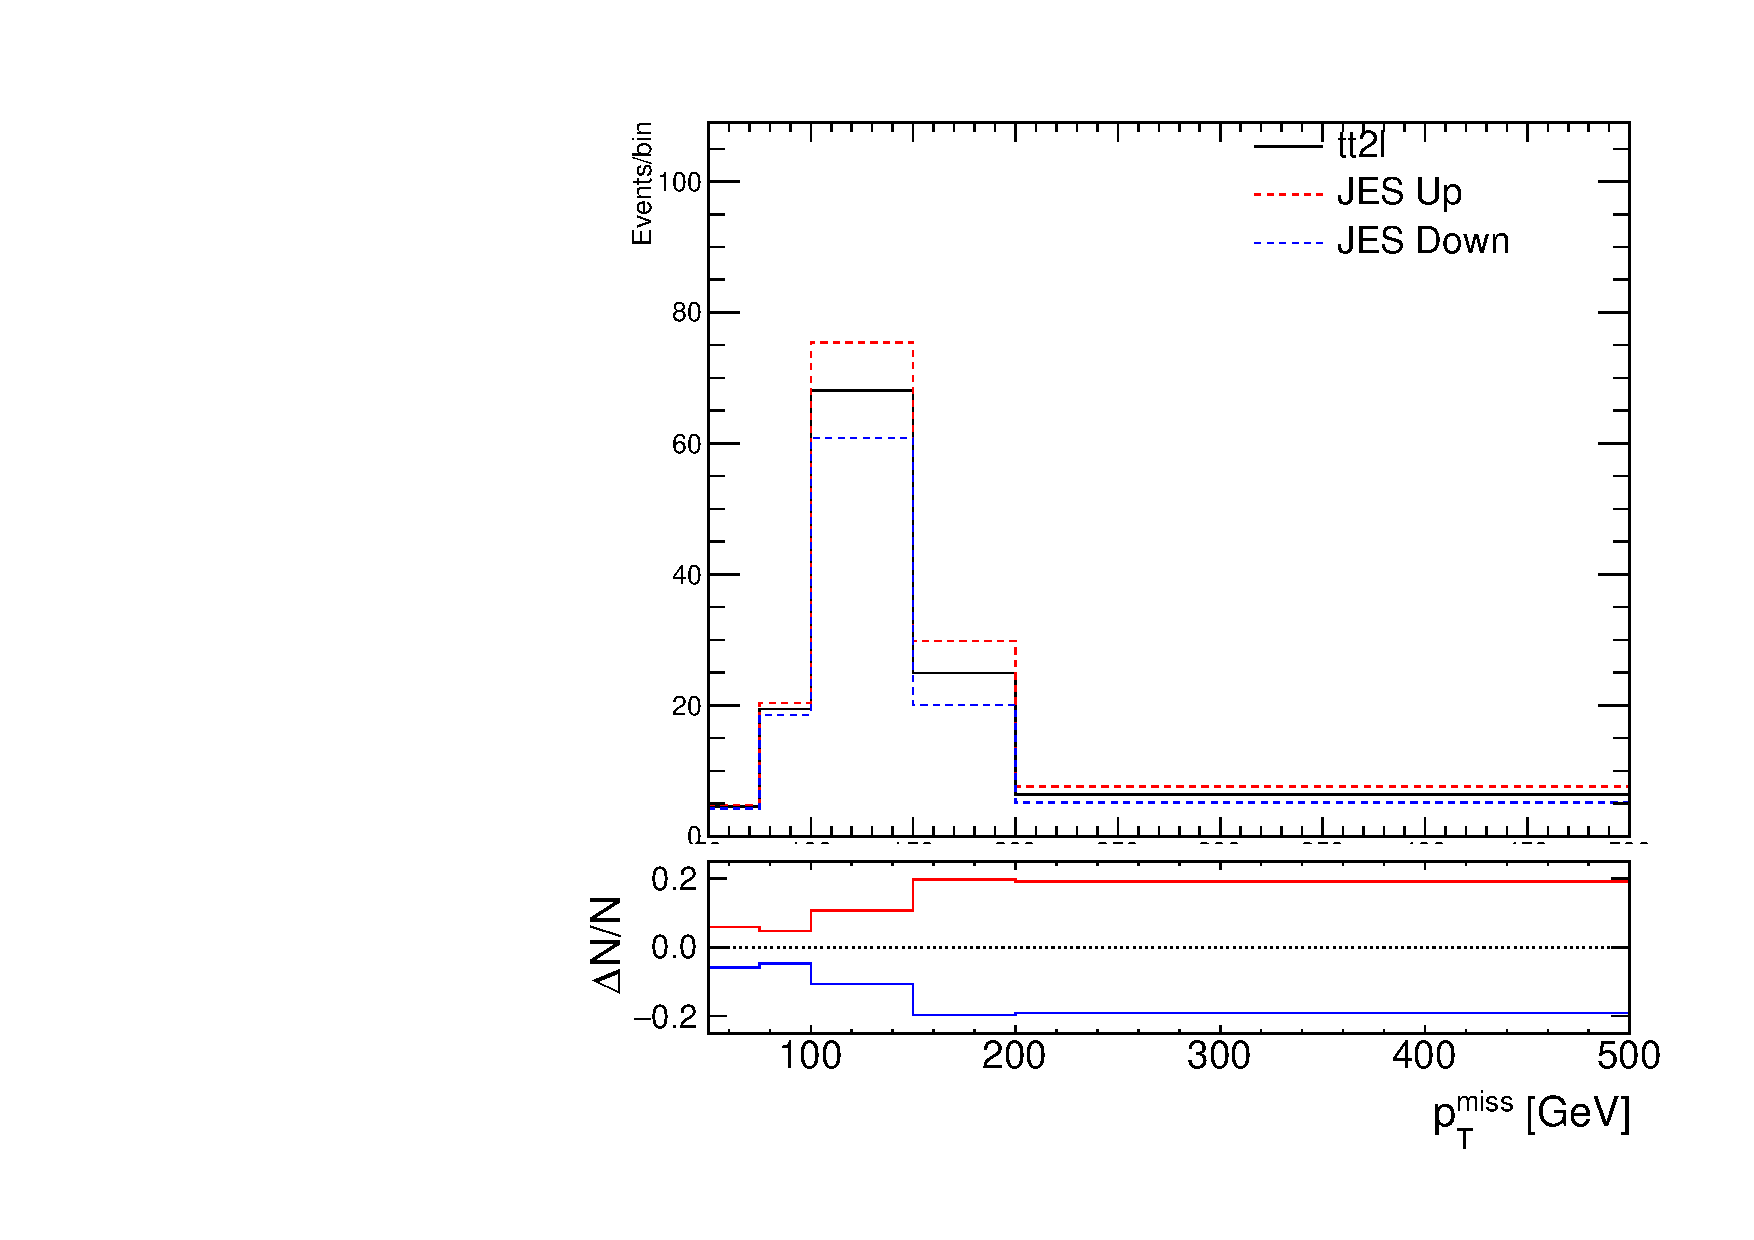
\includegraphics[width=0.48\textwidth]{systs/shapes_ttdm805101_em_hi/tt2l_CMS_scale_j}}
  \caption{The variation in the \ptmiss spectra for \ttll in the low and high \mttll SRs due to the variation of the JES uncertainty by $+1\sigma$ (red) and $-1\sigma$ (blue). The normalized residuals of the ``up'' and ``down'' shapes are shown in the lower panel.}
  \label{fig:JESshape}
\end{figure}

\begin{figure}[h]
  \centering
%  \subfloat[][\ttll, low \mttll-SF]{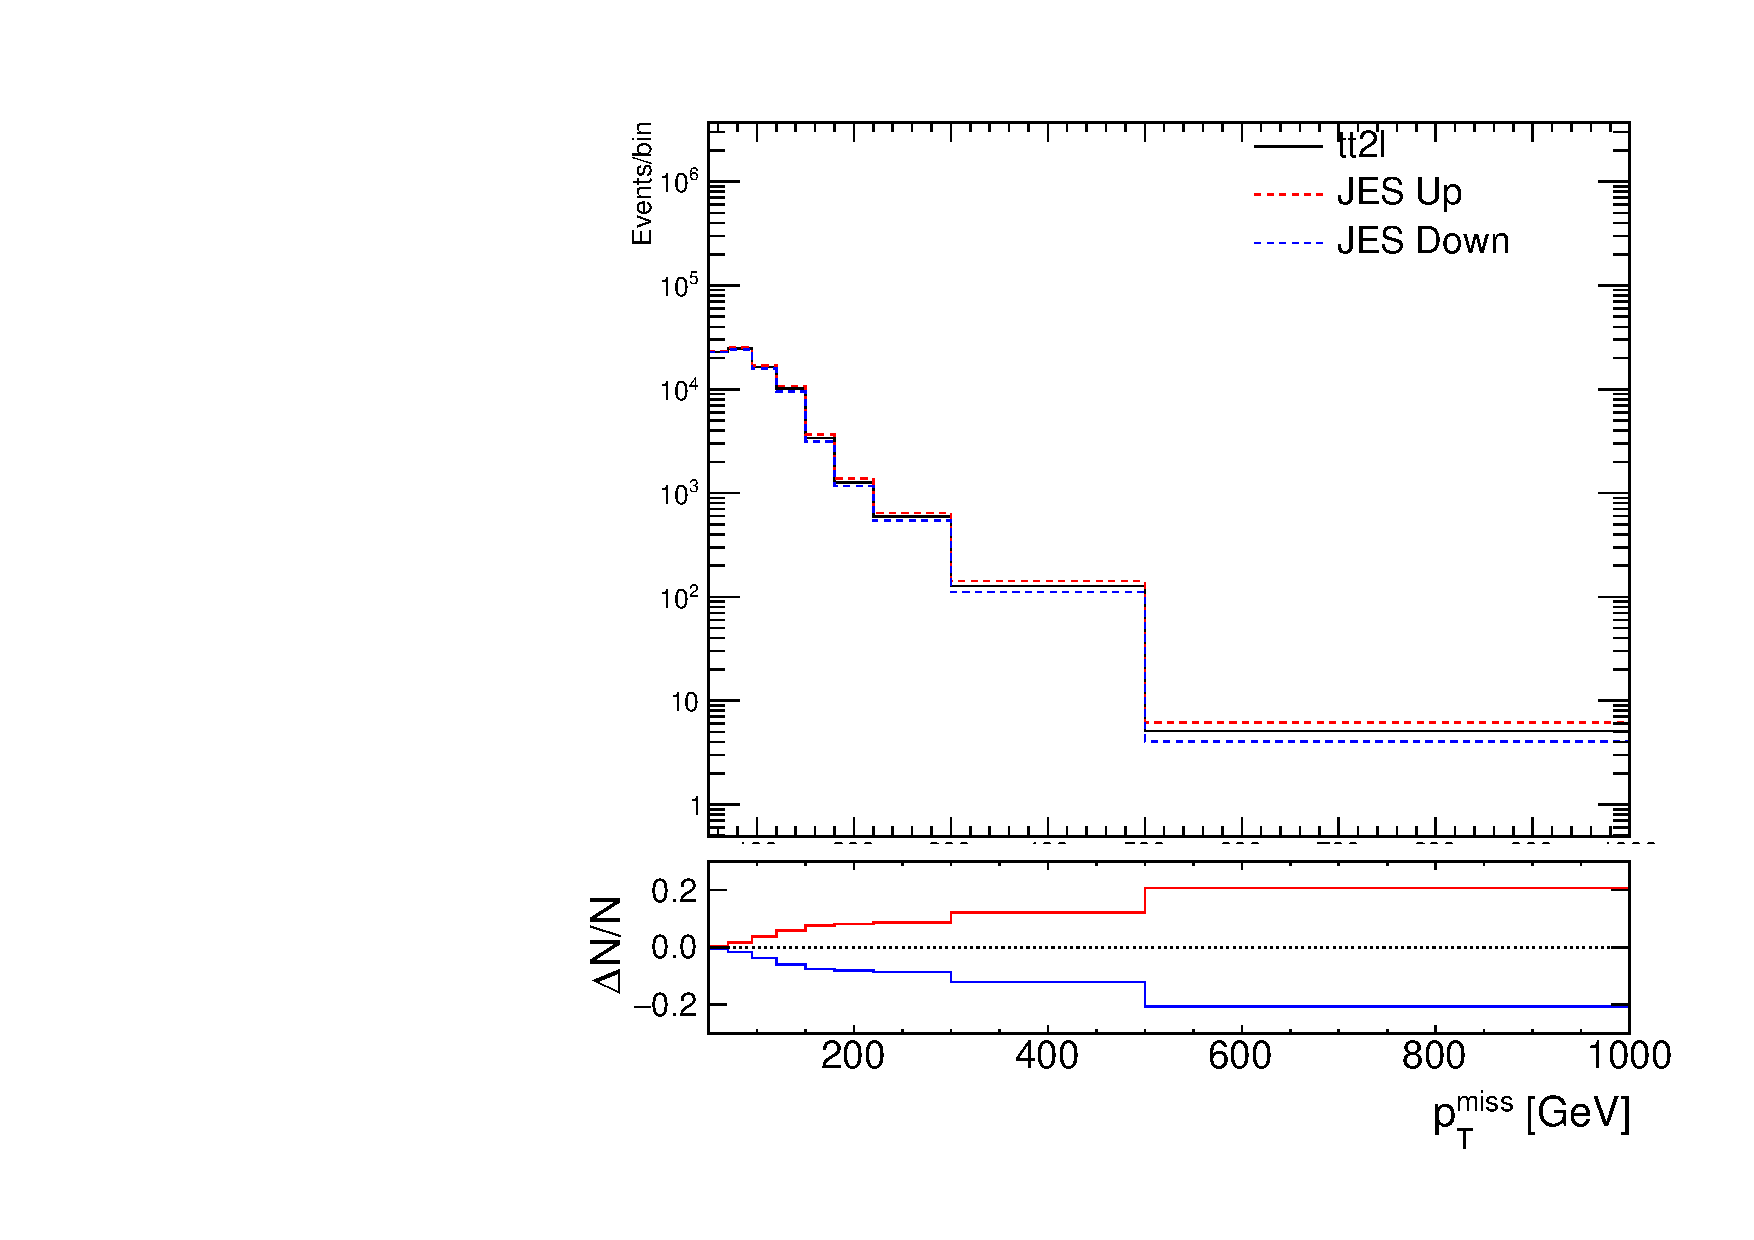
\includegraphics[width=0.48\textwidth]{systs/shapes_ttdm805101_sf_lo/tt2l_CMS_scale_j}}
 % \subfloat[][\ttll, low \mttll-OF]{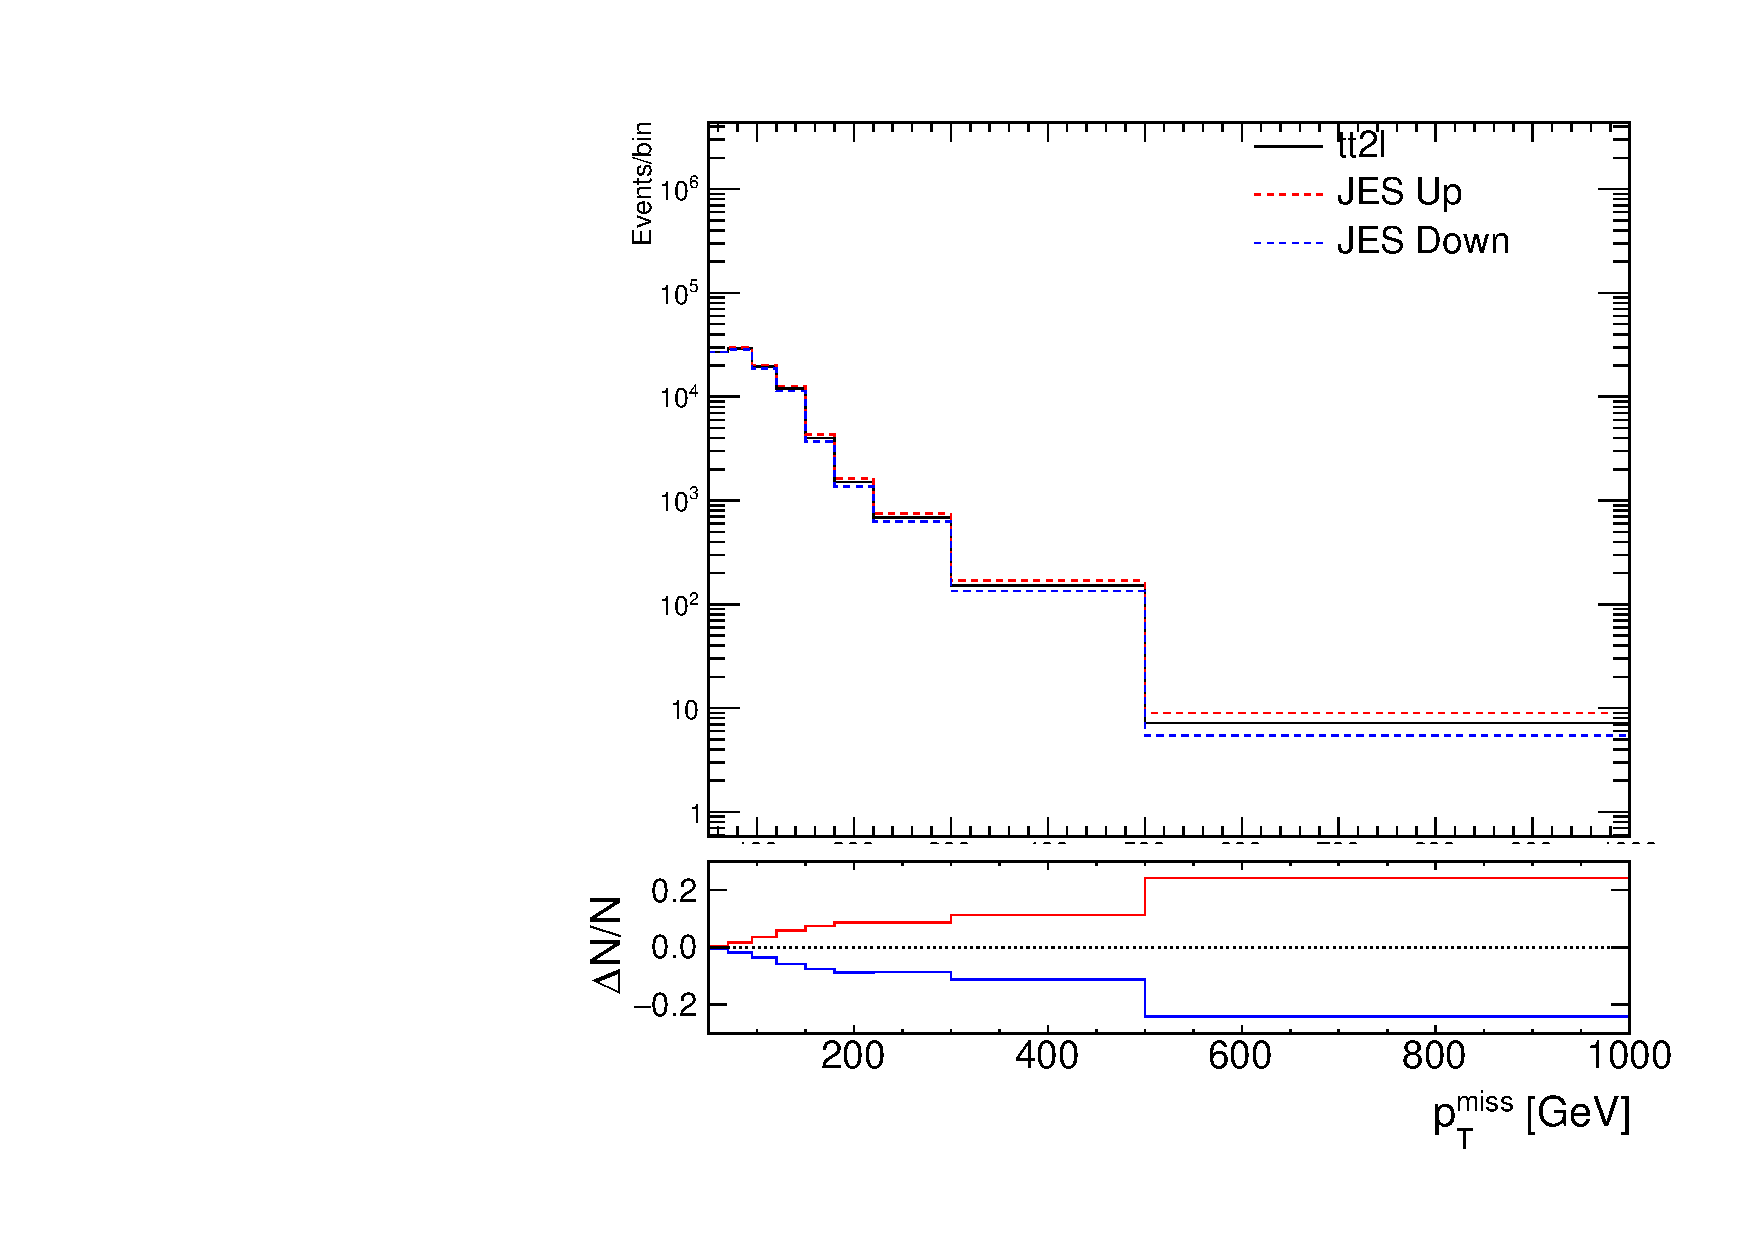
\includegraphics[width=0.48\textwidth]{systs/shapes_ttdm805101_em_lo/tt2l_CMS_scale_j}} \\
  \subfloat[][\ttll, high \mttll-SF]{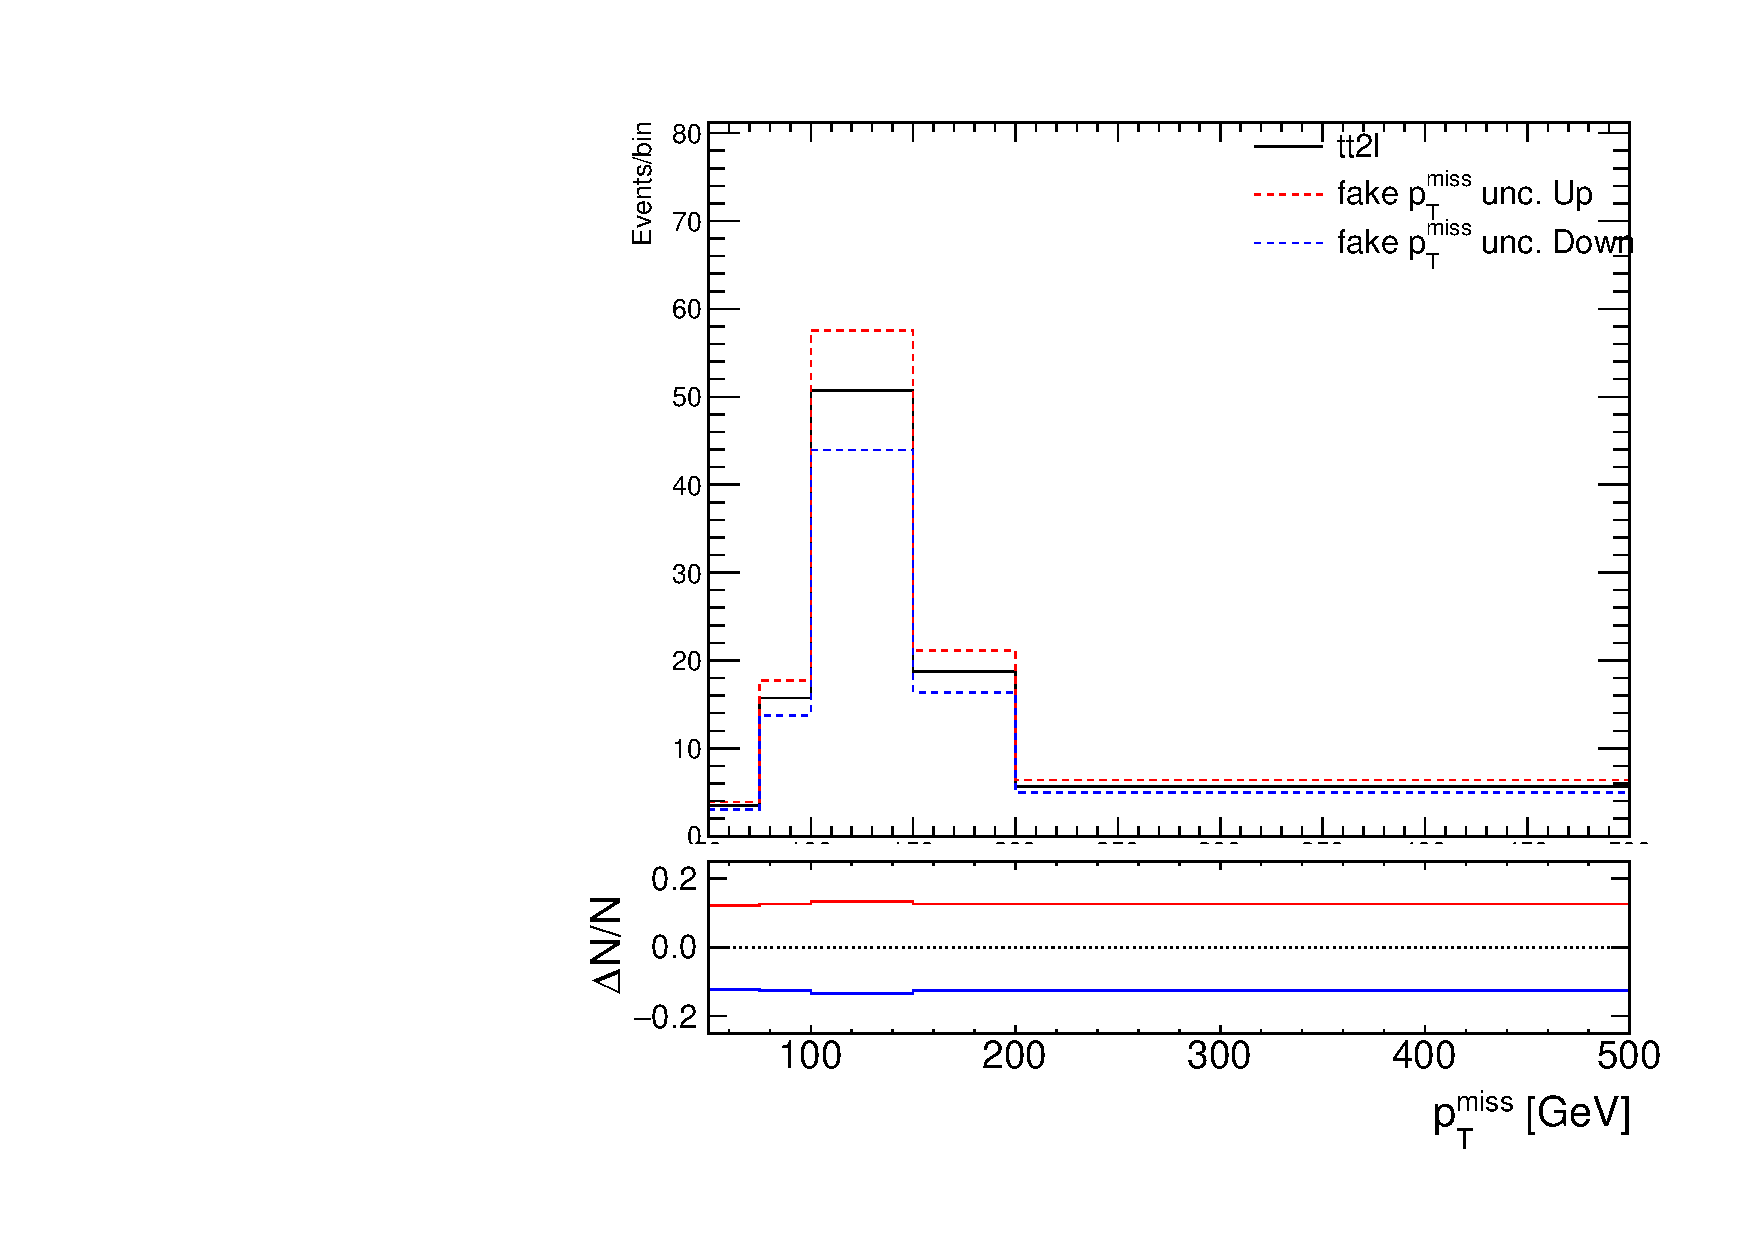
\includegraphics[width=0.48\textwidth]{systs/shapes_ttdm805101_sf_hi/tt2l_RecoilCorr}}
  \subfloat[][\ttll, high \mttll-OF]{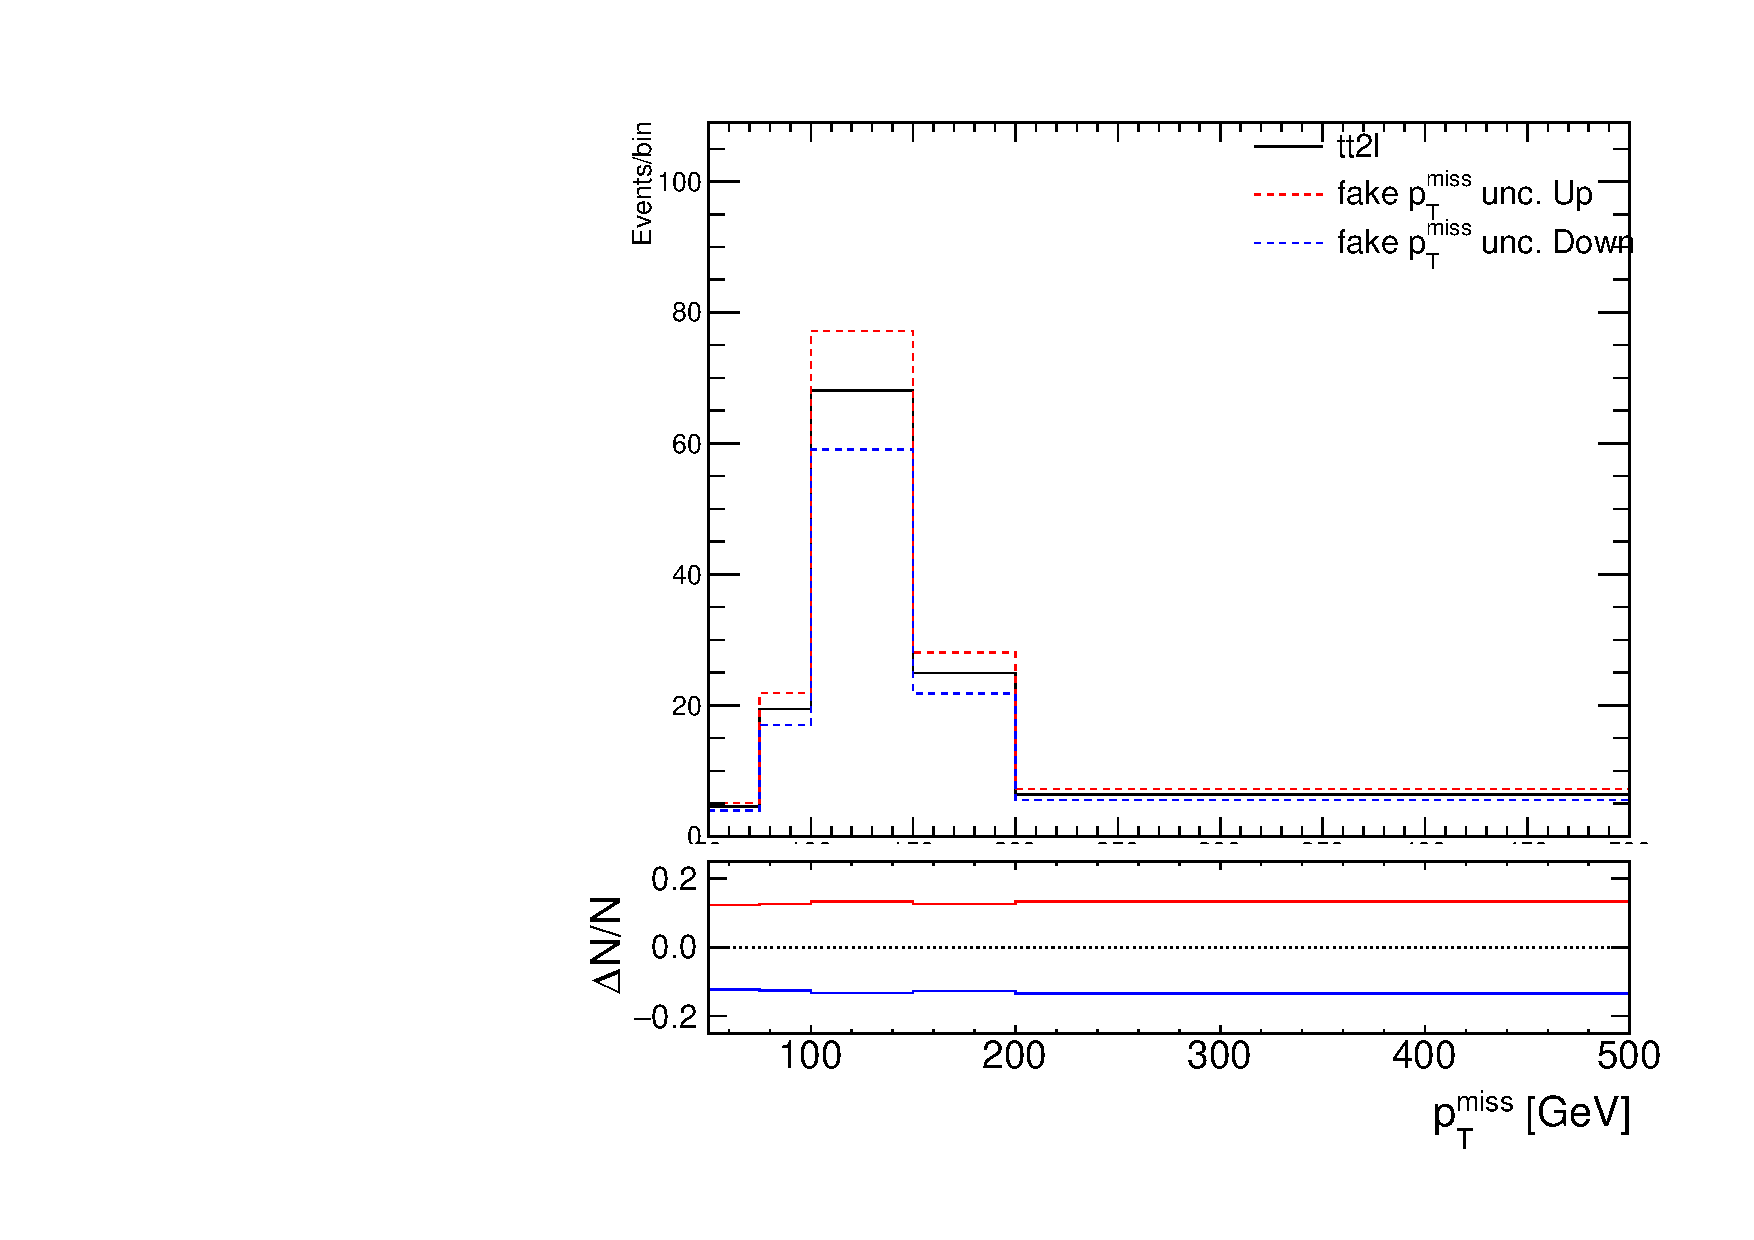
\includegraphics[width=0.48\textwidth]{systs/shapes_ttdm805101_em_hi/tt2l_RecoilCorr}}
  \caption{The variation in the \ptmiss spectra for \ttll in the high \mttll SRs due to the variation of the fake \ptmiss uncertainty by $+1\sigma$ (red) and $-1\sigma$ (blue). The normalized residuals of the ``up'' and ``down'' shapes are shown in the lower panel.}
  \label{fig:fakeMETshape}
\end{figure}

\begin{figure}[h]
  \centering
  \subfloat[][\ttll, low \mttll-SF]{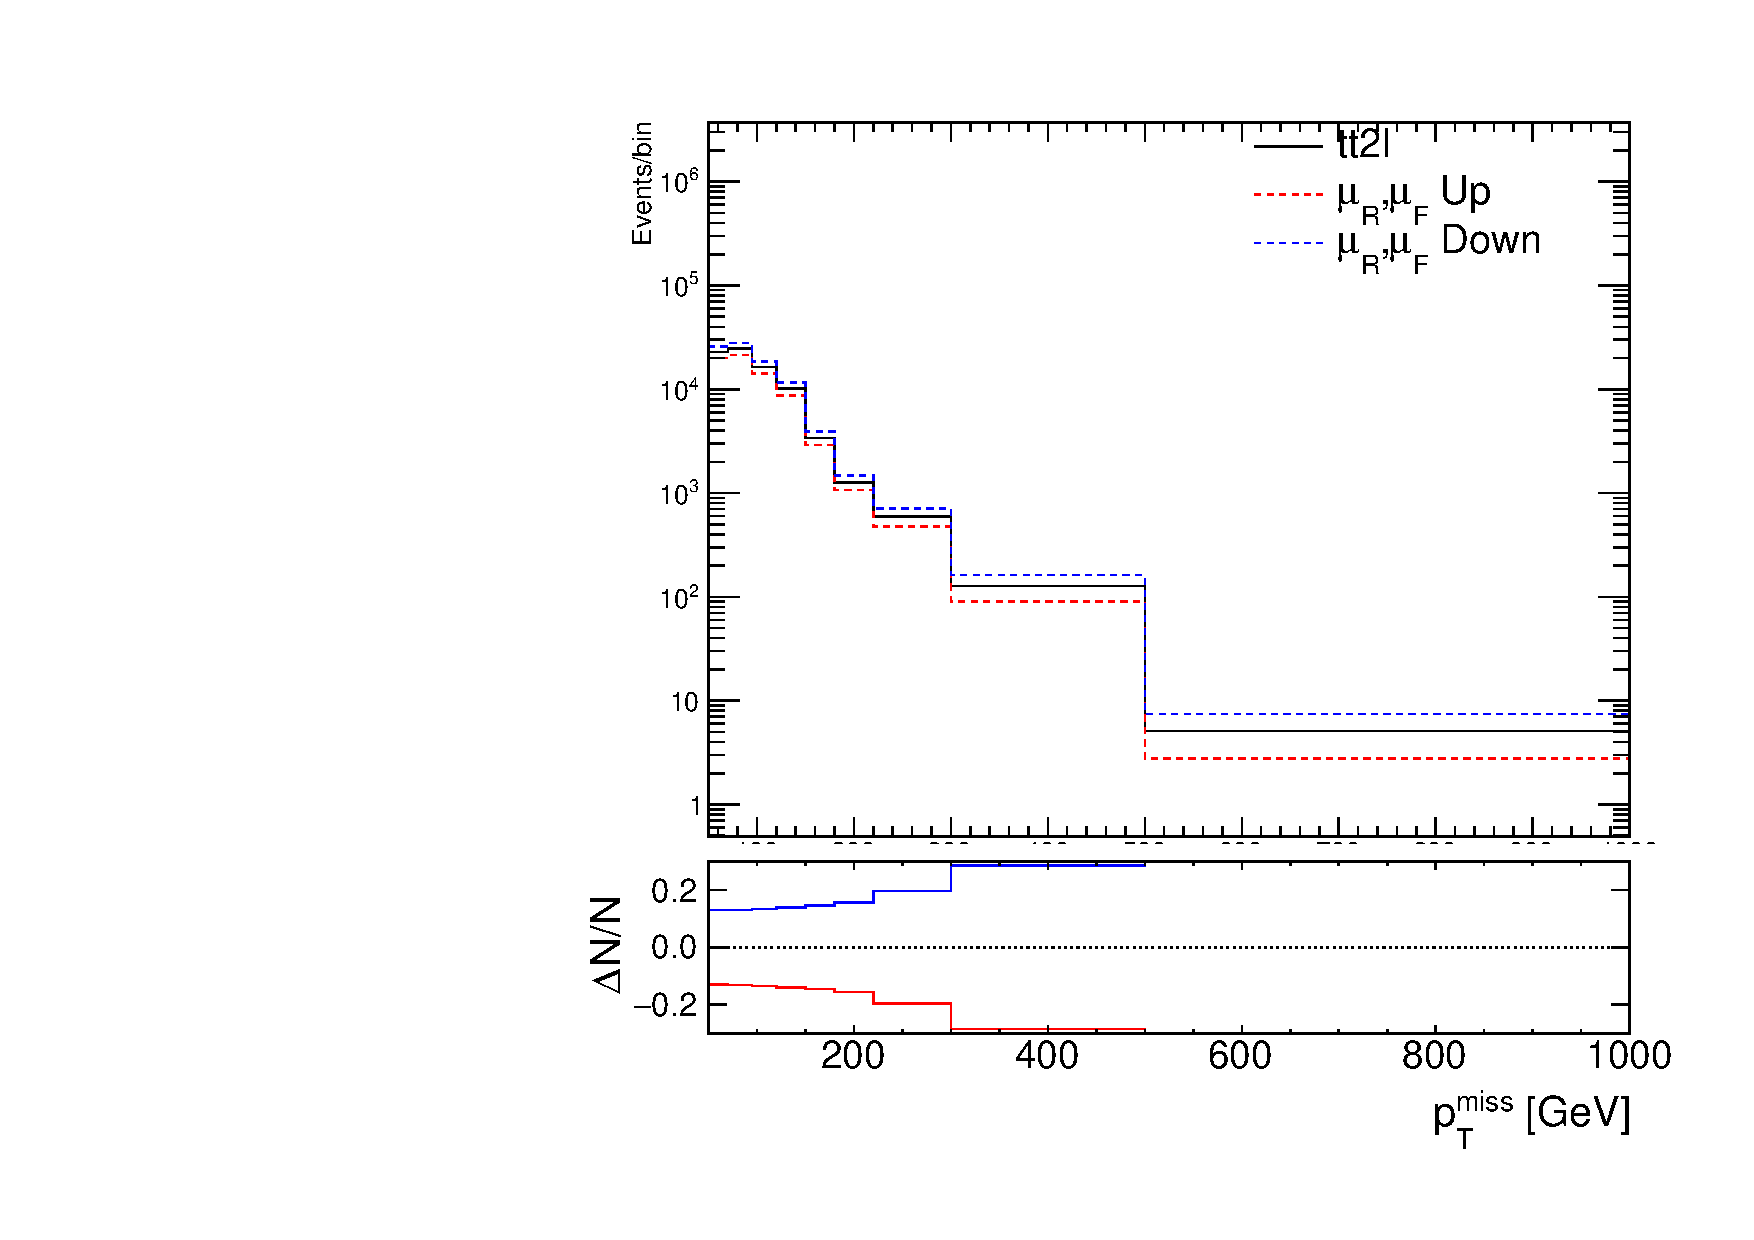
\includegraphics[width=0.48\textwidth]{systs/shapes_ttdm805101_sf_lo/tt2l_tt_qcdScale}}
  \subfloat[][\ttll, low \mttll-OF]{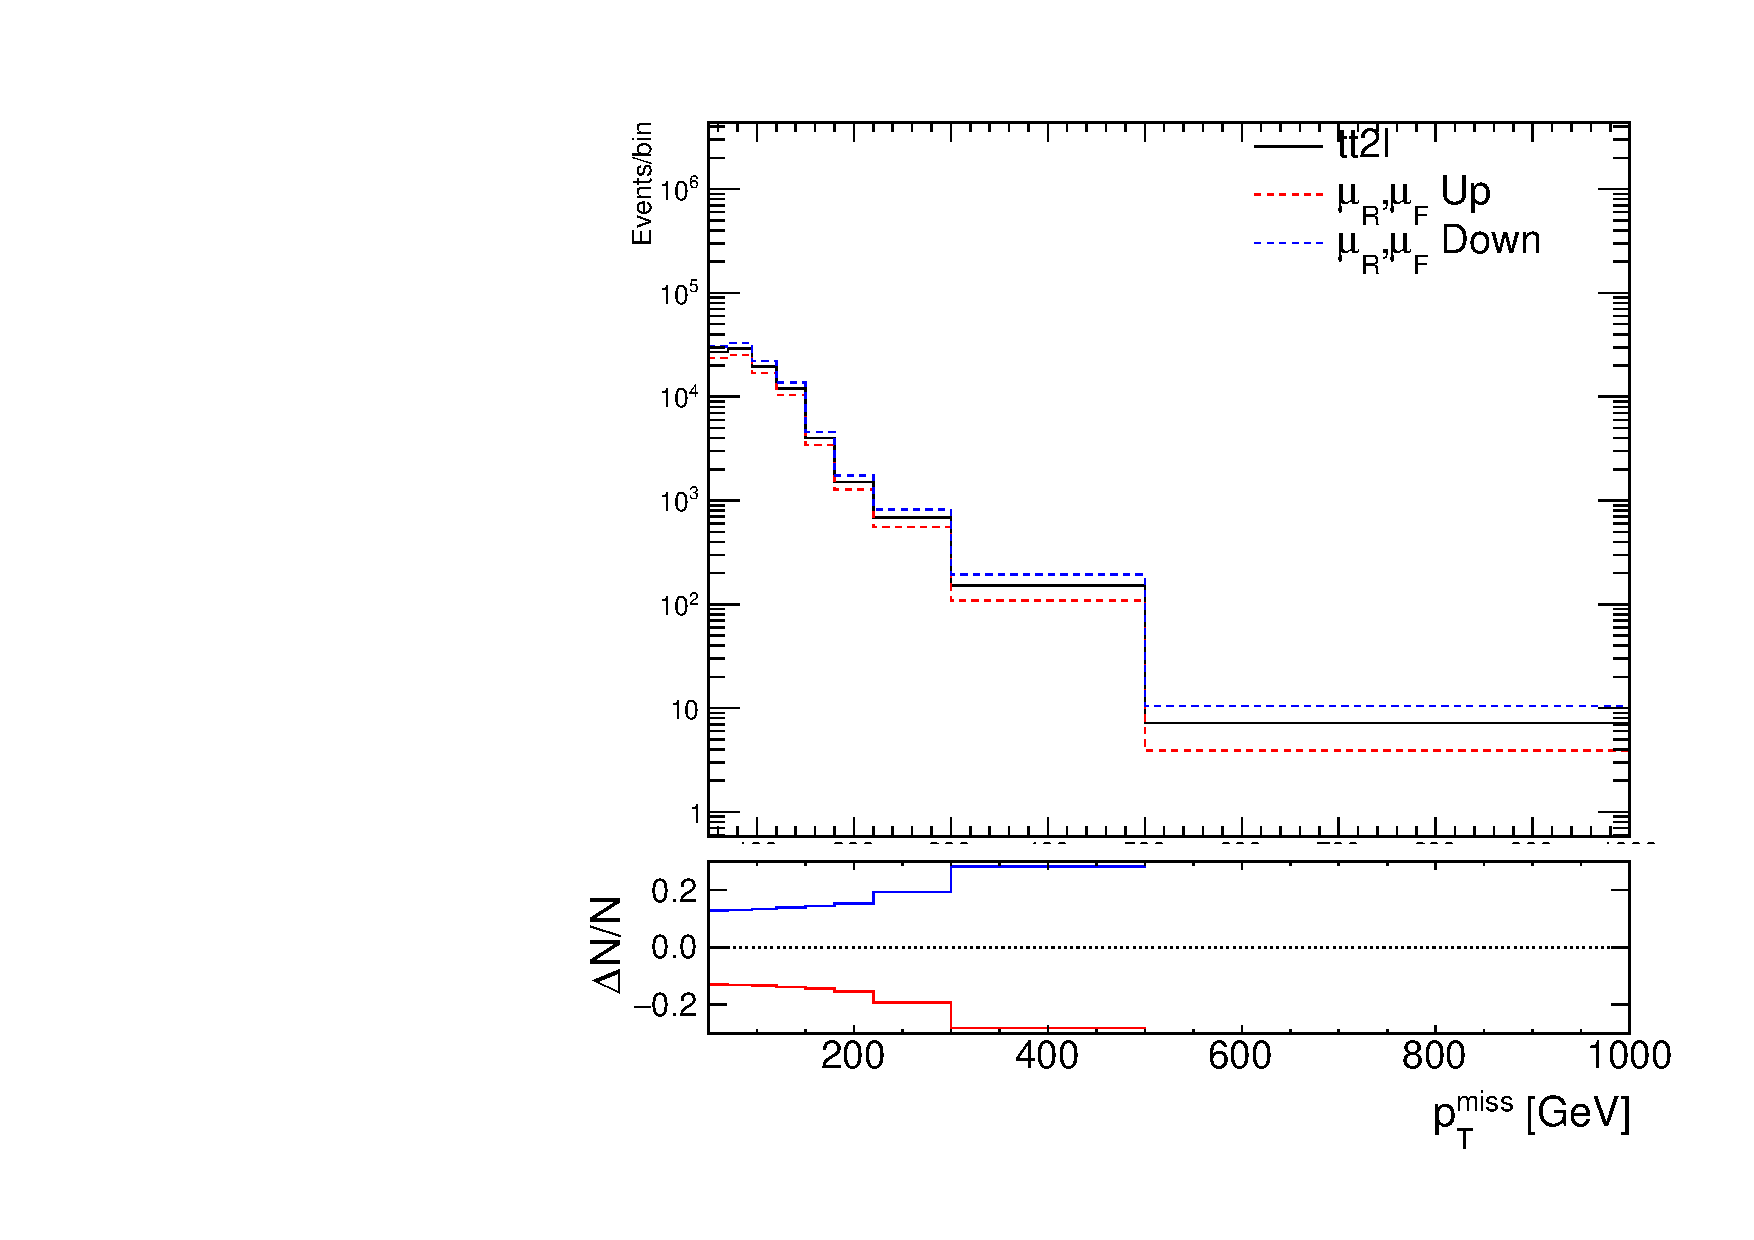
\includegraphics[width=0.48\textwidth]{systs/shapes_ttdm805101_em_lo/tt2l_tt_qcdScale}} \\
  \subfloat[][\ttll, high \mttll-SF]{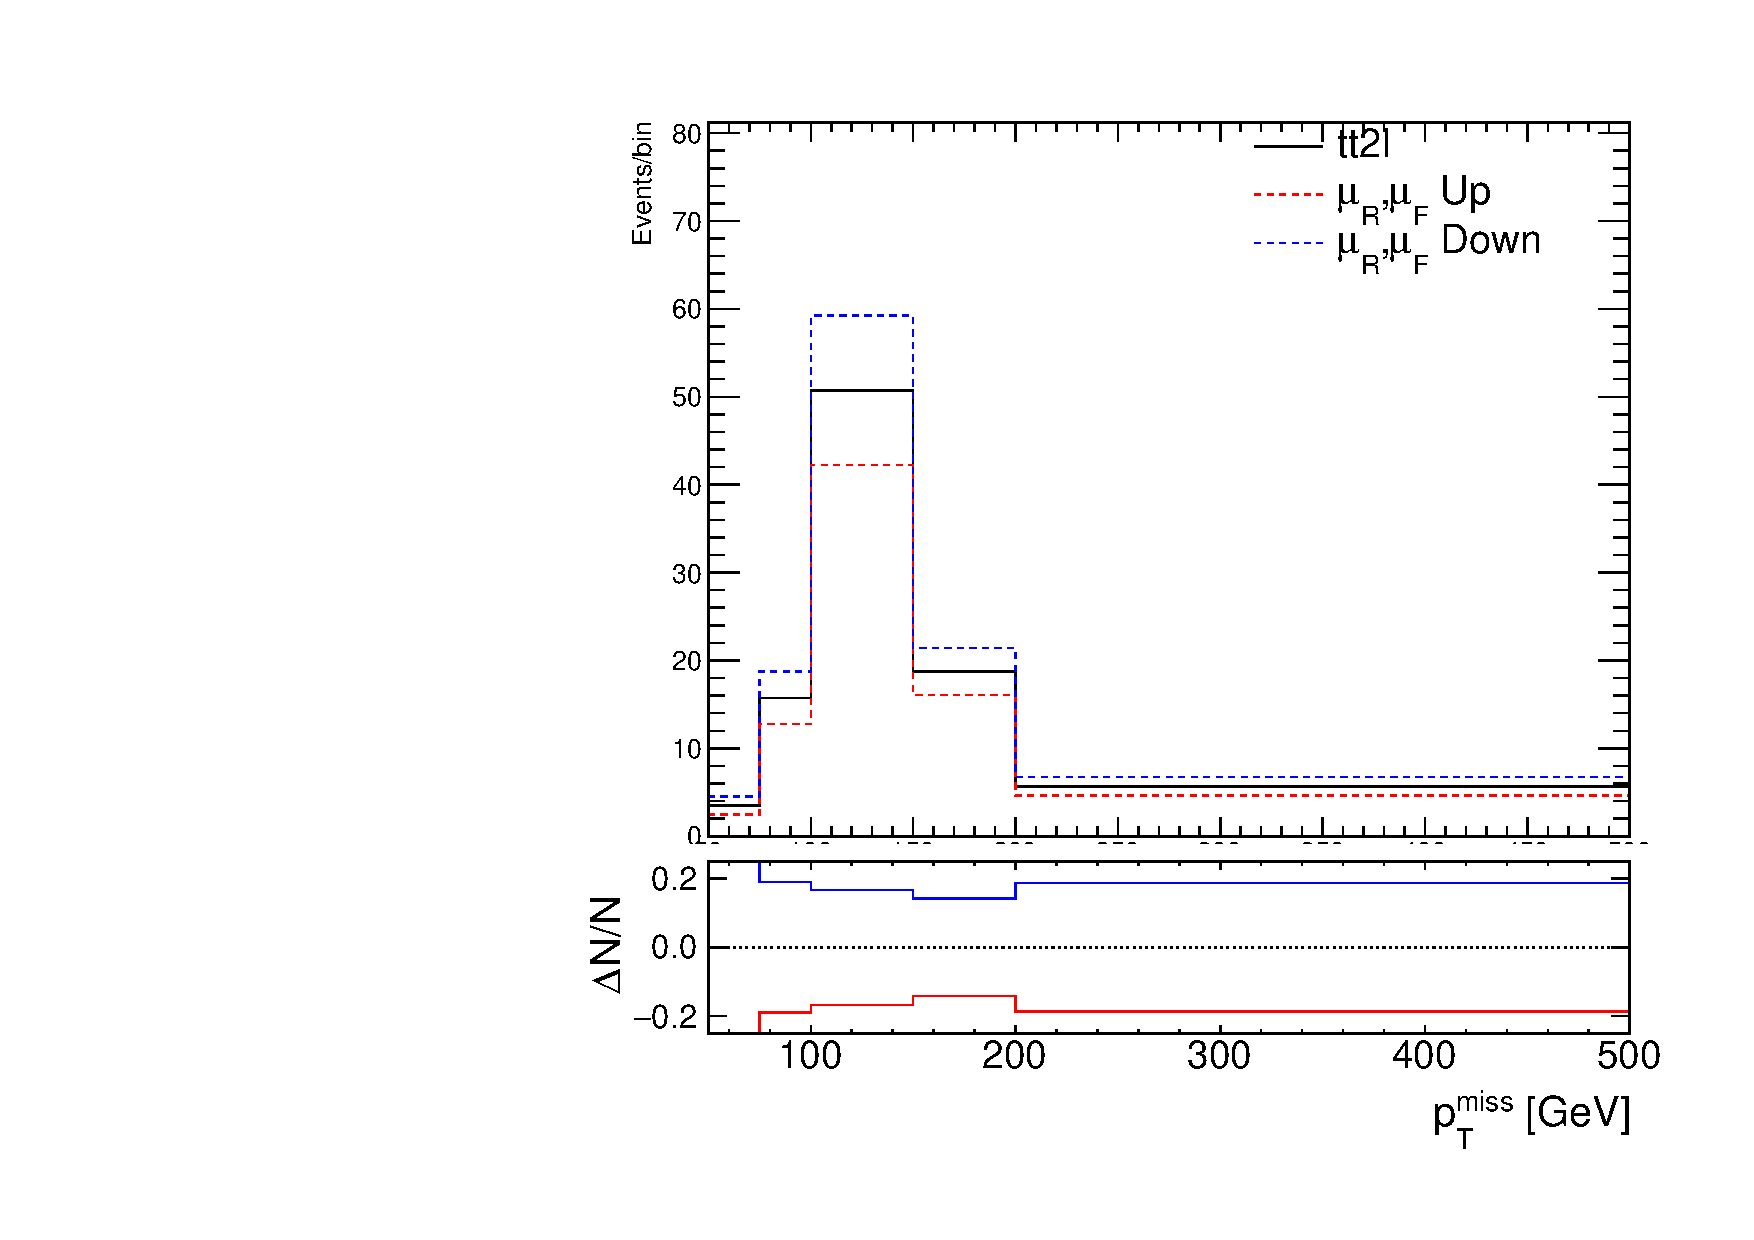
\includegraphics[width=0.48\textwidth]{systs/shapes_ttdm805101_sf_hi/tt2l_tt_qcdScale}}
  \subfloat[][\ttll, high \mttll-OF]{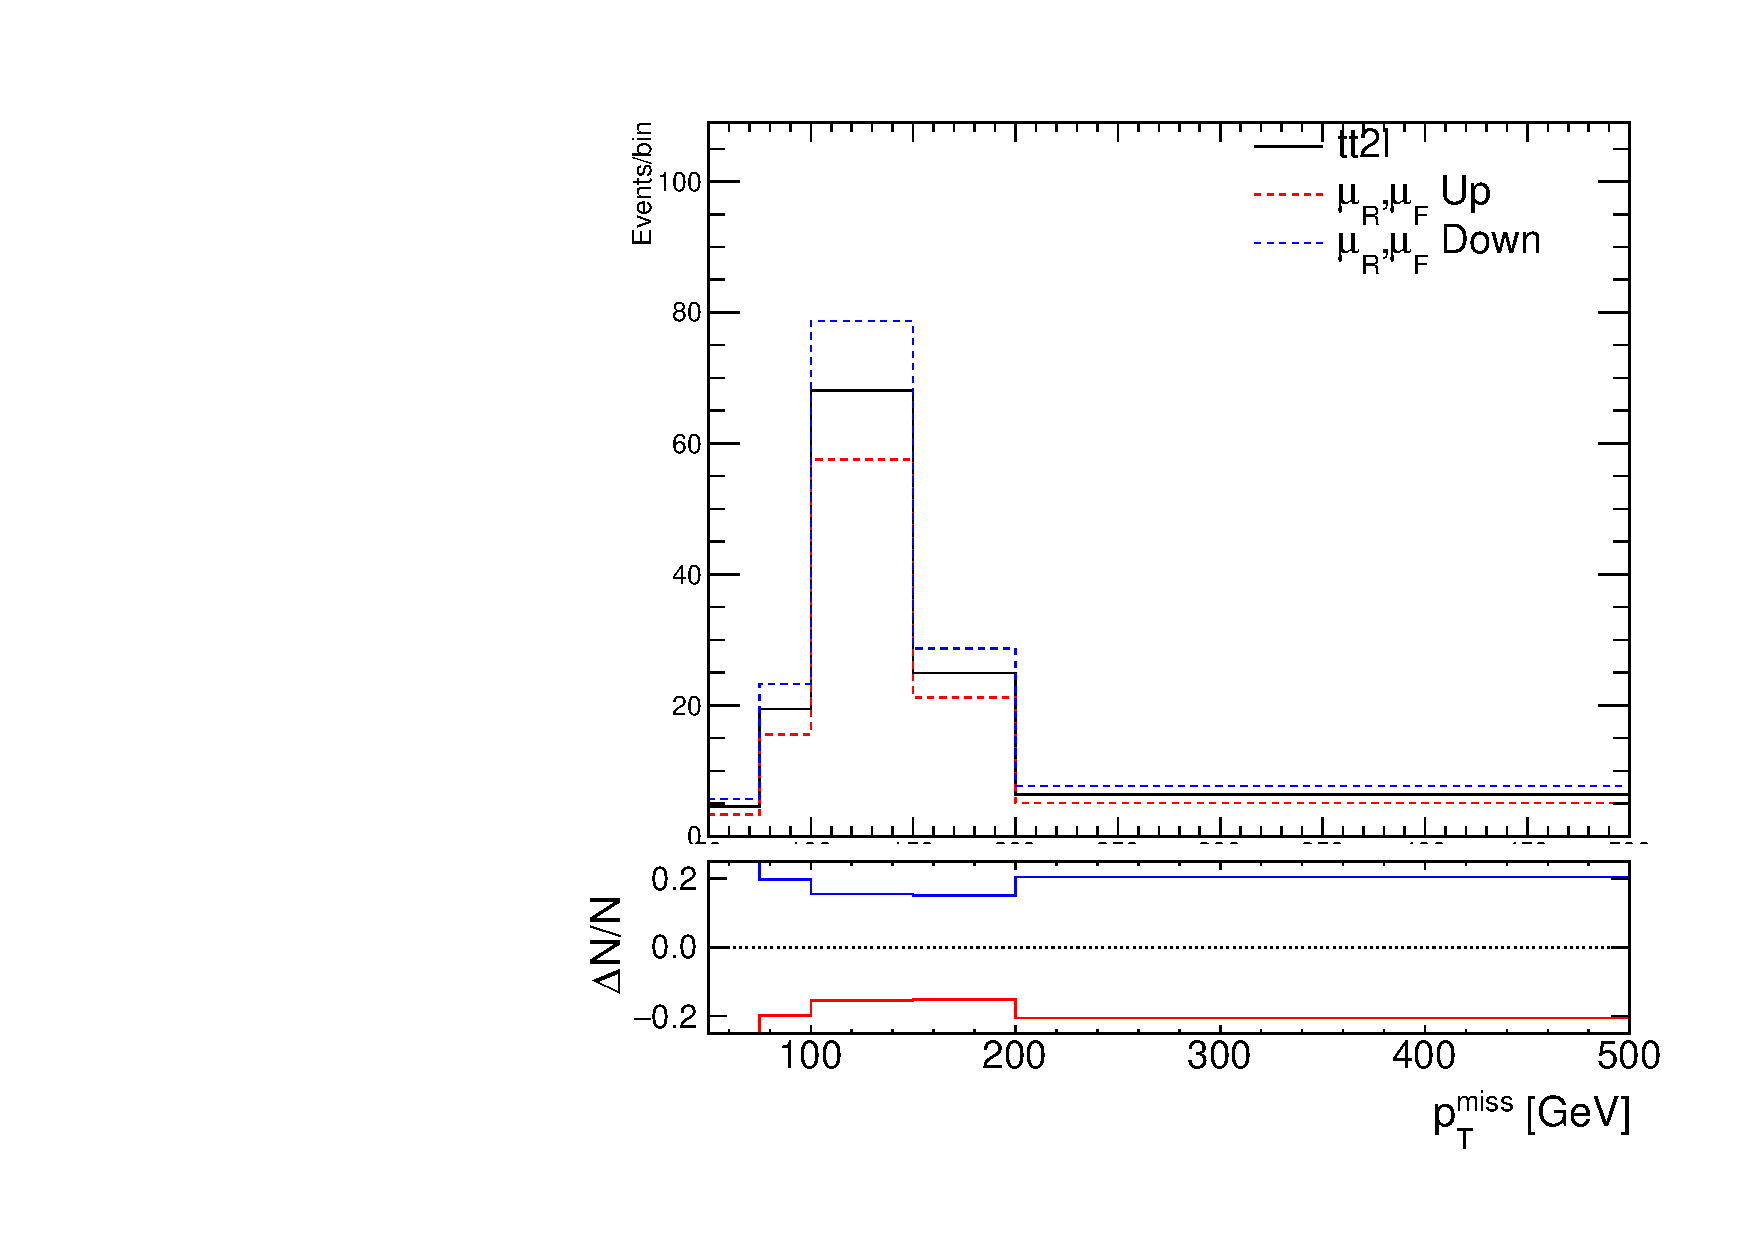
\includegraphics[width=0.48\textwidth]{systs/shapes_ttdm805101_em_hi/tt2l_tt_qcdScale}}
  \caption{The variation in the \ptmiss spectra for \ttll in the low and high \mttll SRs due to the variation of the factorization and renormalization scales by $+1\sigma$ (red) and $-1\sigma$ (blue). The normalized residuals of the ``up'' and ``down'' shapes are shown in the lower panel.}
  \label{fig:ttQCDshape}
\end{figure}

\begin{figure}[h]
  \centering
  \subfloat[][\ttll, low \mttll-SF]{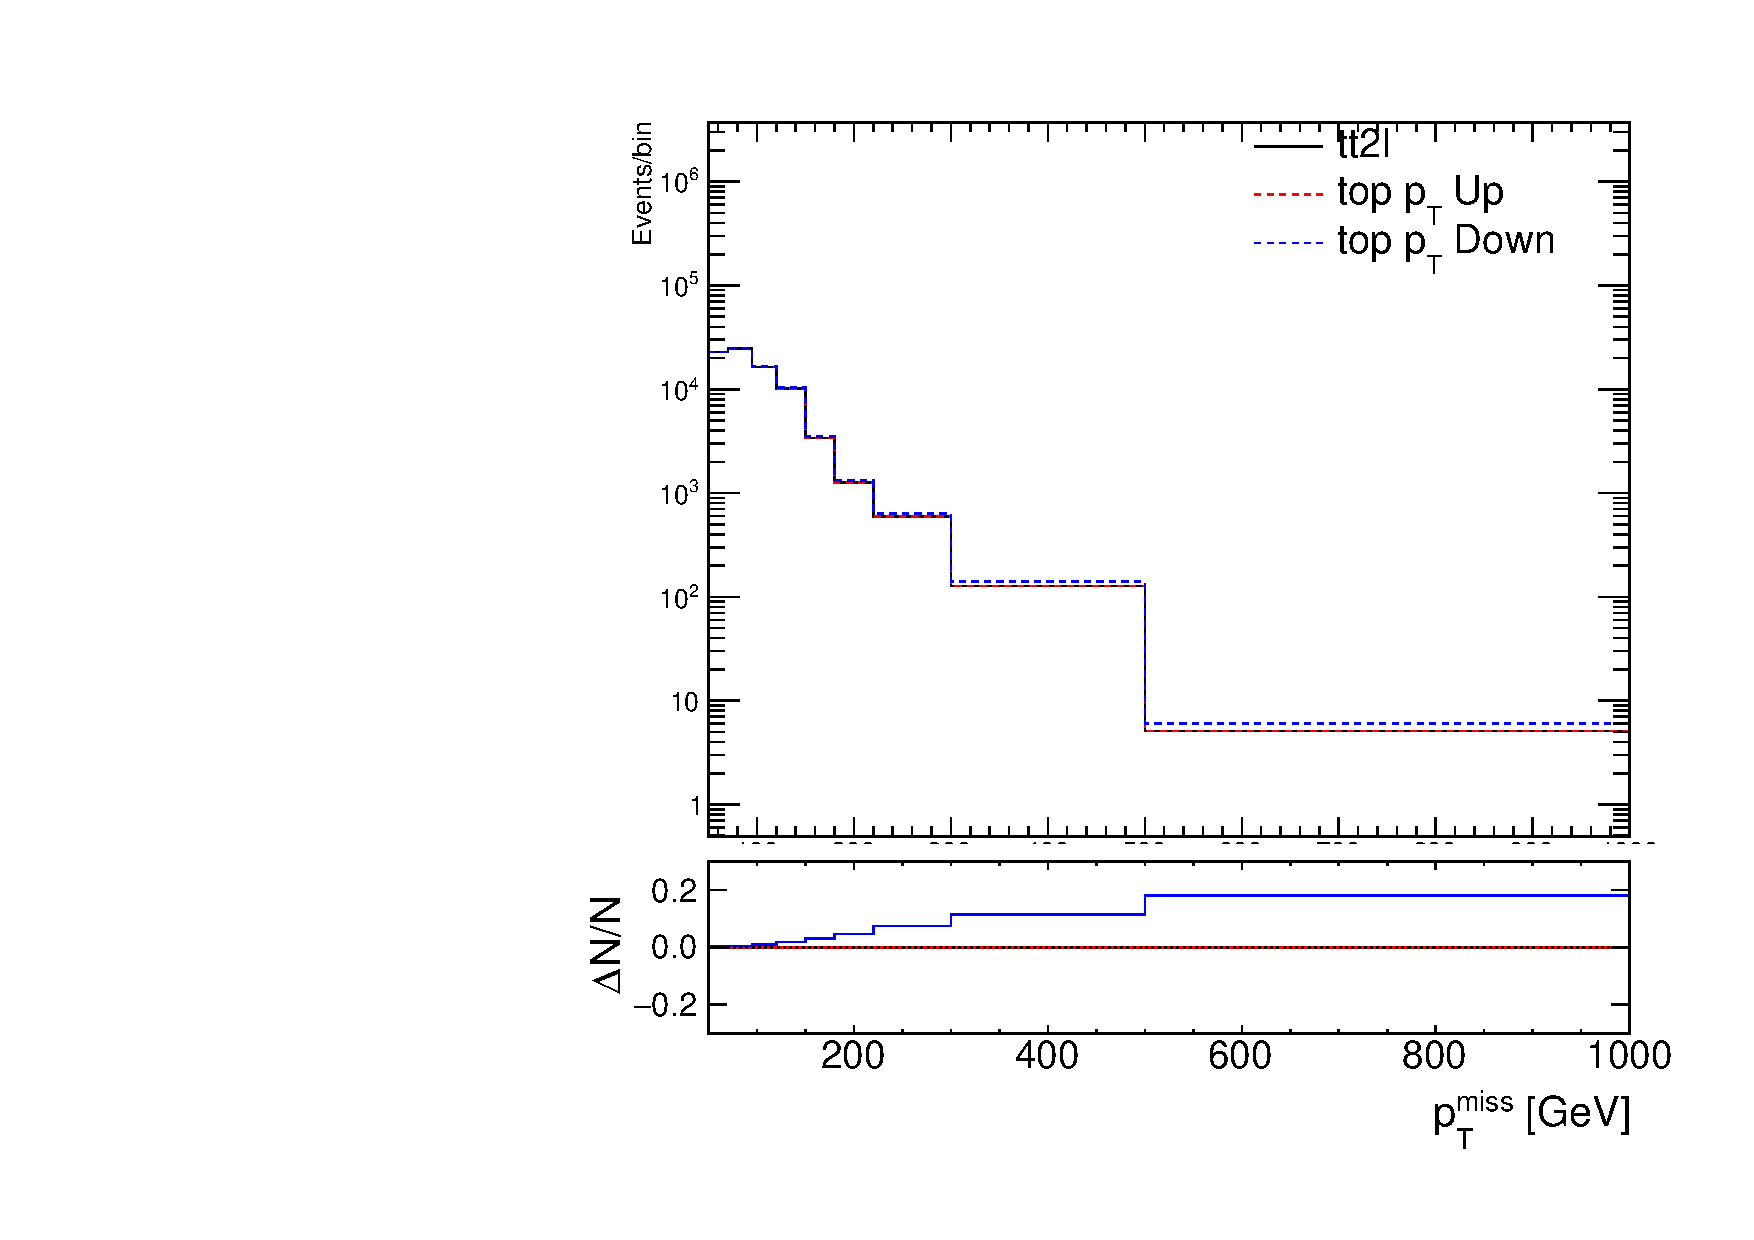
\includegraphics[width=0.48\textwidth]{systs/shapes_ttdm805101_sf_lo/tt2l_topPt}}
  \subfloat[][\ttll, low \mttll-OF]{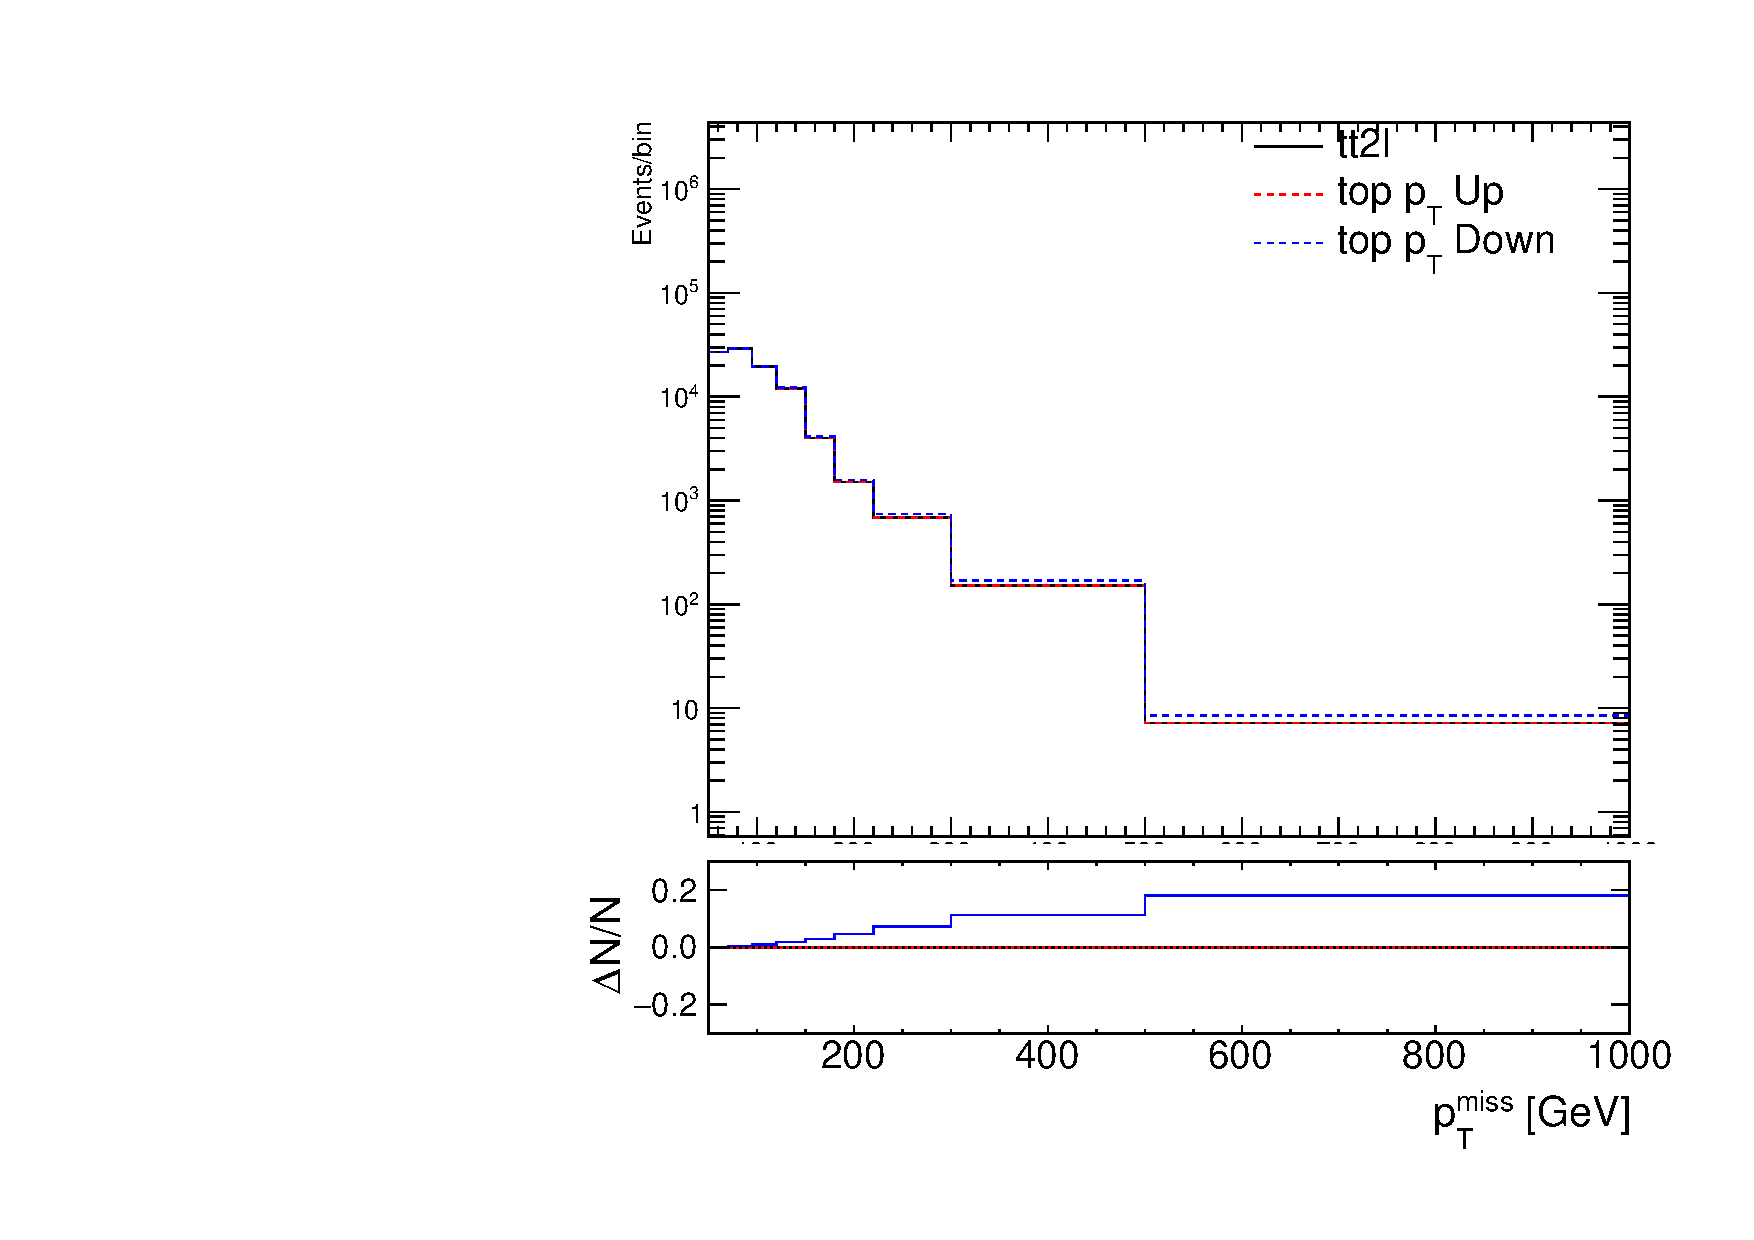
\includegraphics[width=0.48\textwidth]{systs/shapes_ttdm805101_em_lo/tt2l_topPt}} \\
  \subfloat[][\ttll, high \mttll-SF]{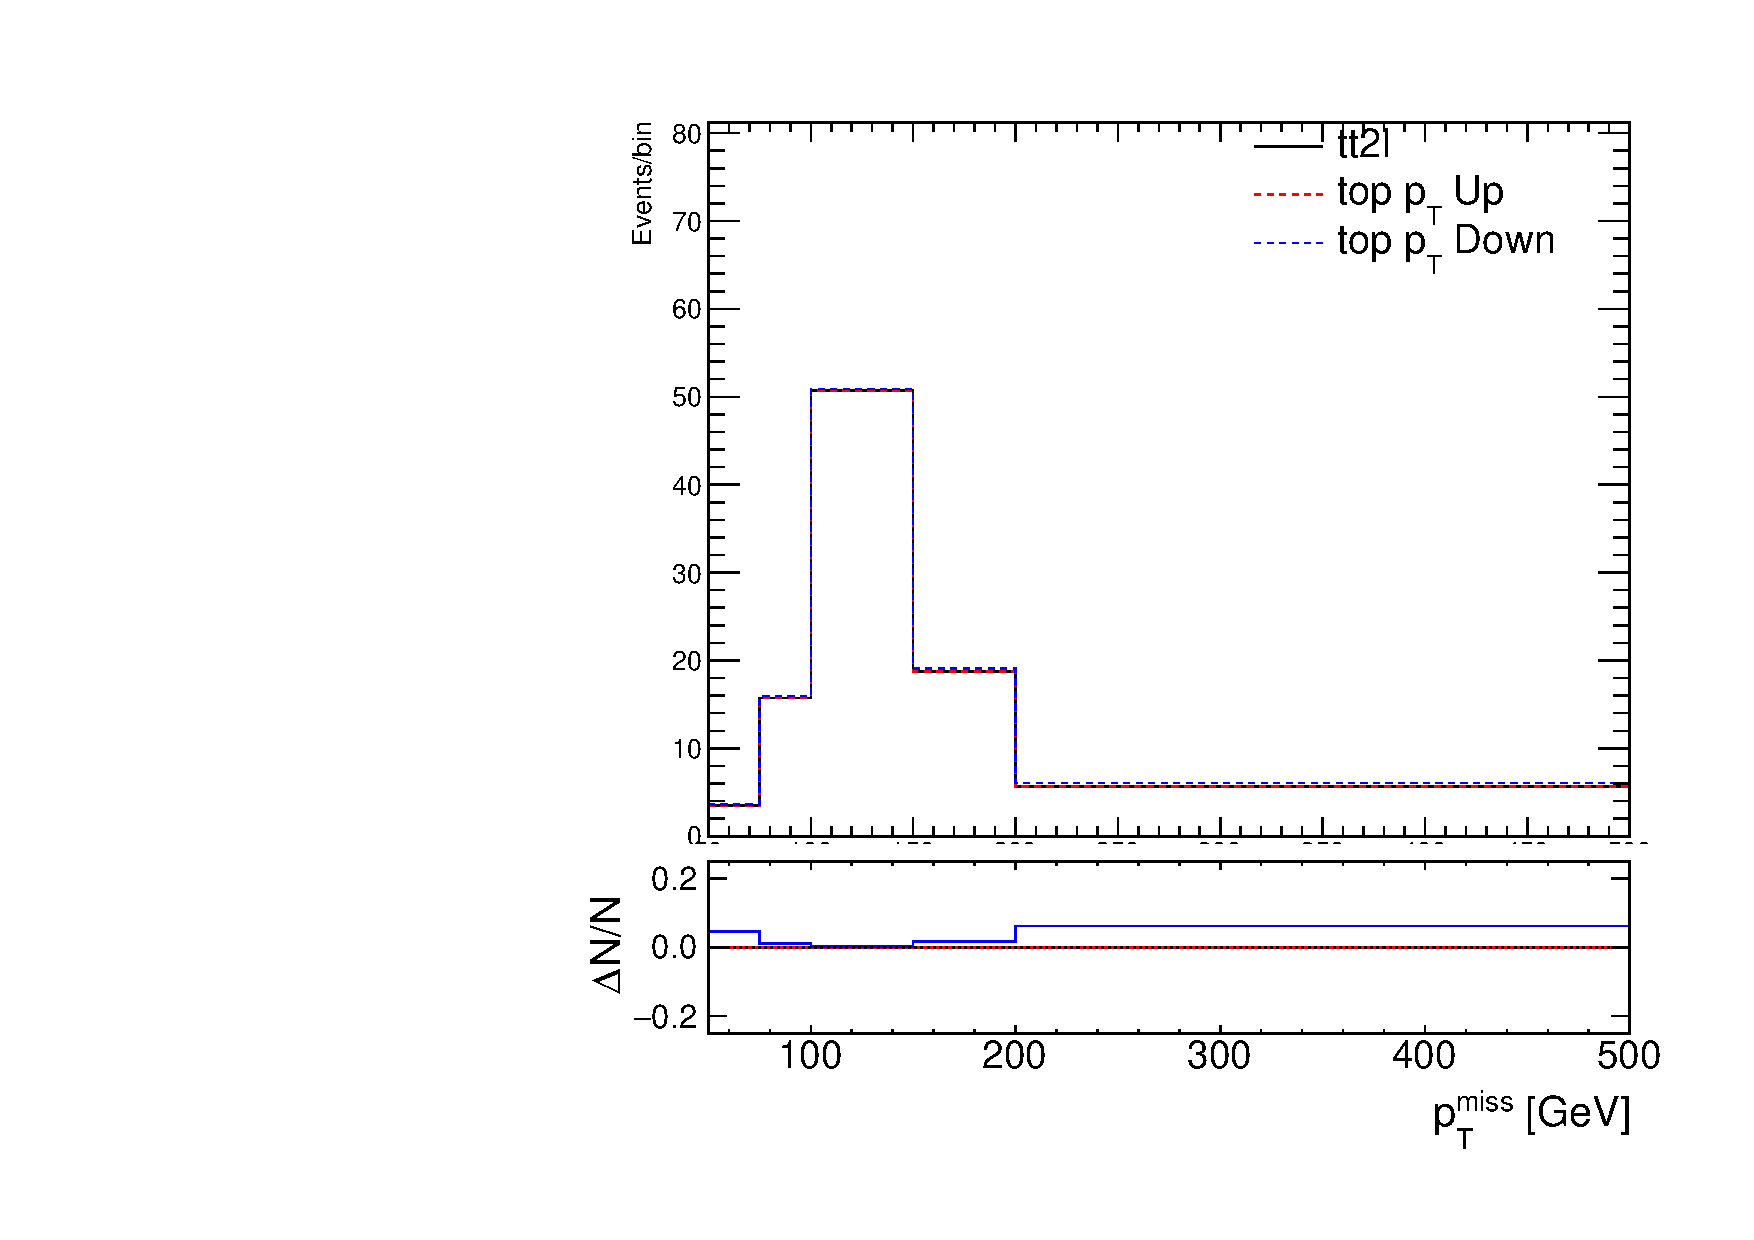
\includegraphics[width=0.48\textwidth]{systs/shapes_ttdm805101_sf_hi/tt2l_topPt}}
  \subfloat[][\ttll, high \mttll-OF]{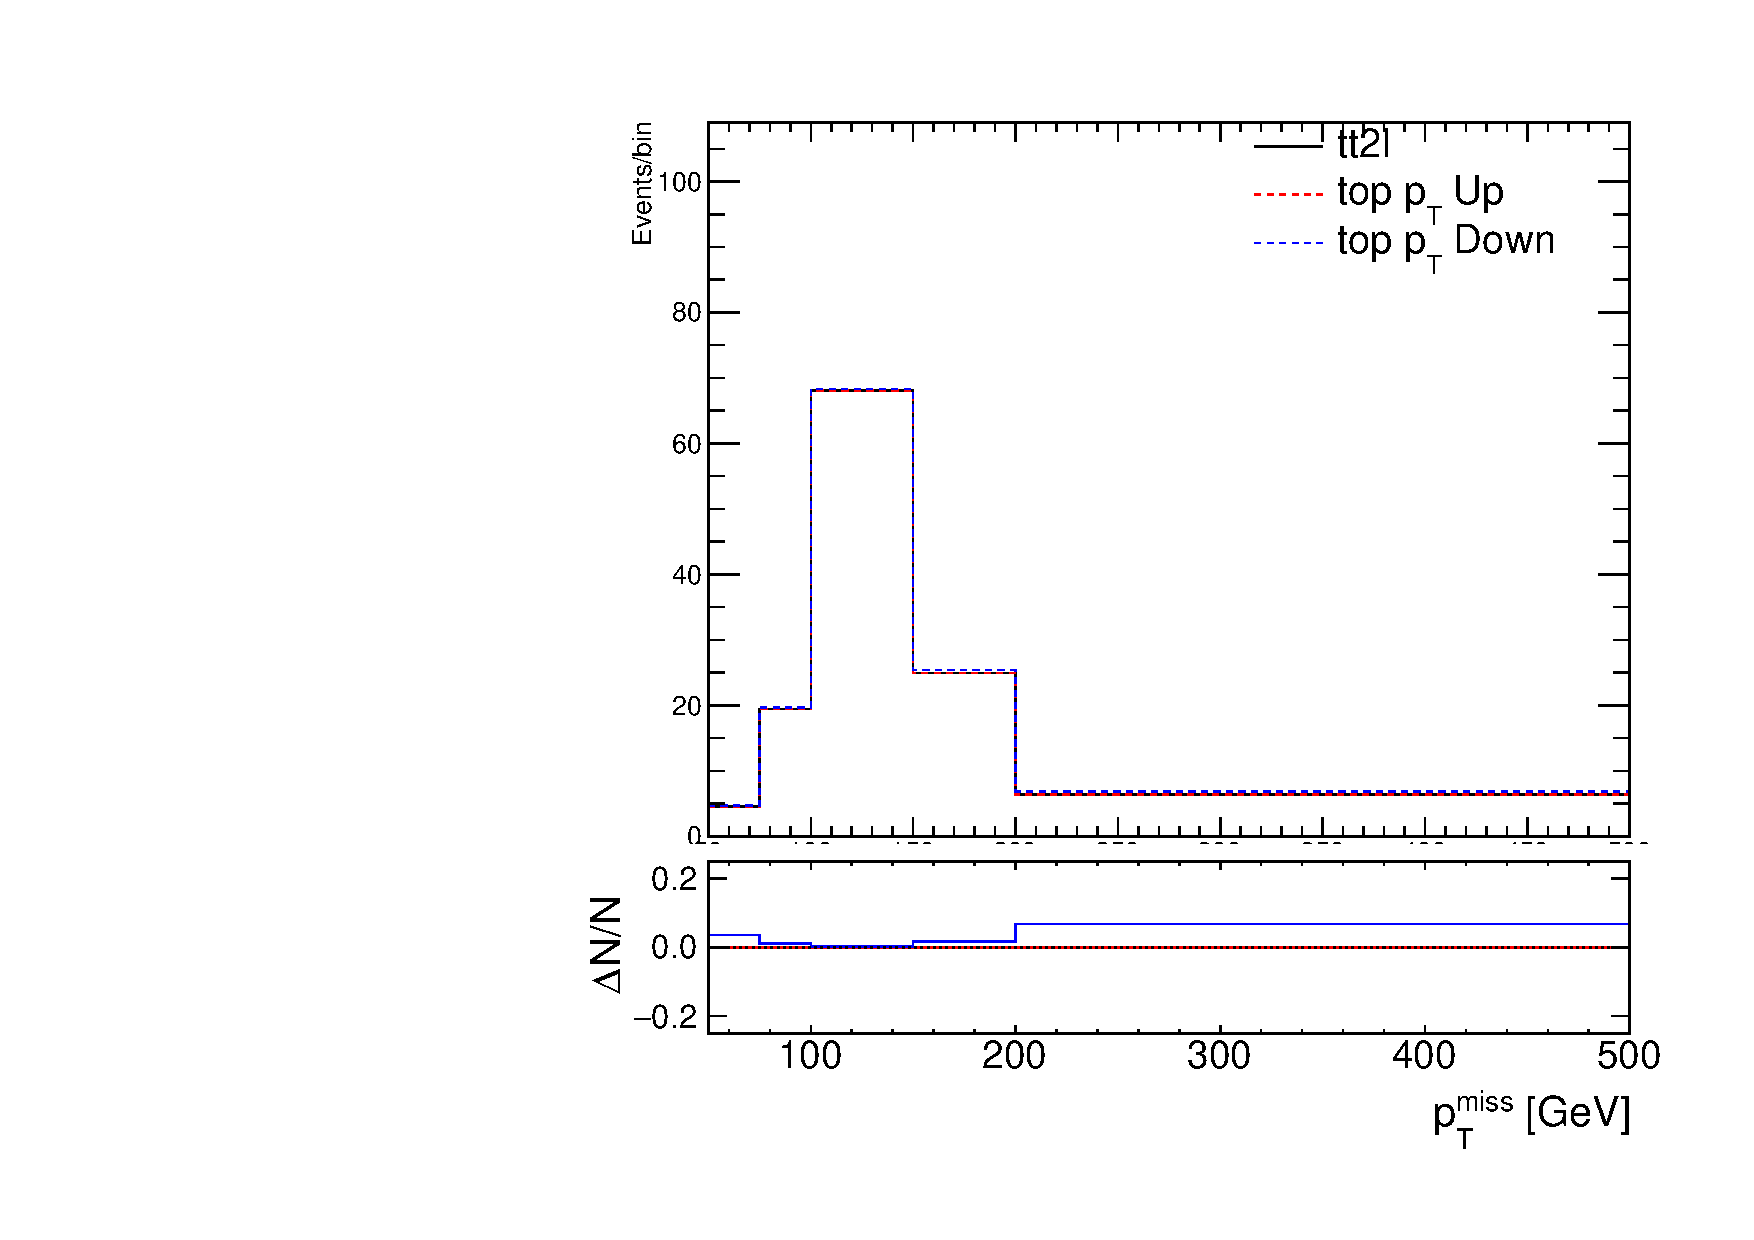
\includegraphics[width=0.48\textwidth]{systs/shapes_ttdm805101_em_hi/tt2l_topPt}}
  \caption{The variation in the \ptmiss spectra for \ttll in the low and high \mttll SRs due to the variation of top quark \pt by $+1\sigma$ (red) and $-1\sigma$ (blue) of the uncertainty. The normalized residuals of the ``up'' and ``down'' shapes are shown in the lower panel.}
  \label{fig:topPtshape}
\end{figure}

\begin{figure}[h]
  \centering
  \subfloat[][\ttll, low \mttll-SF]{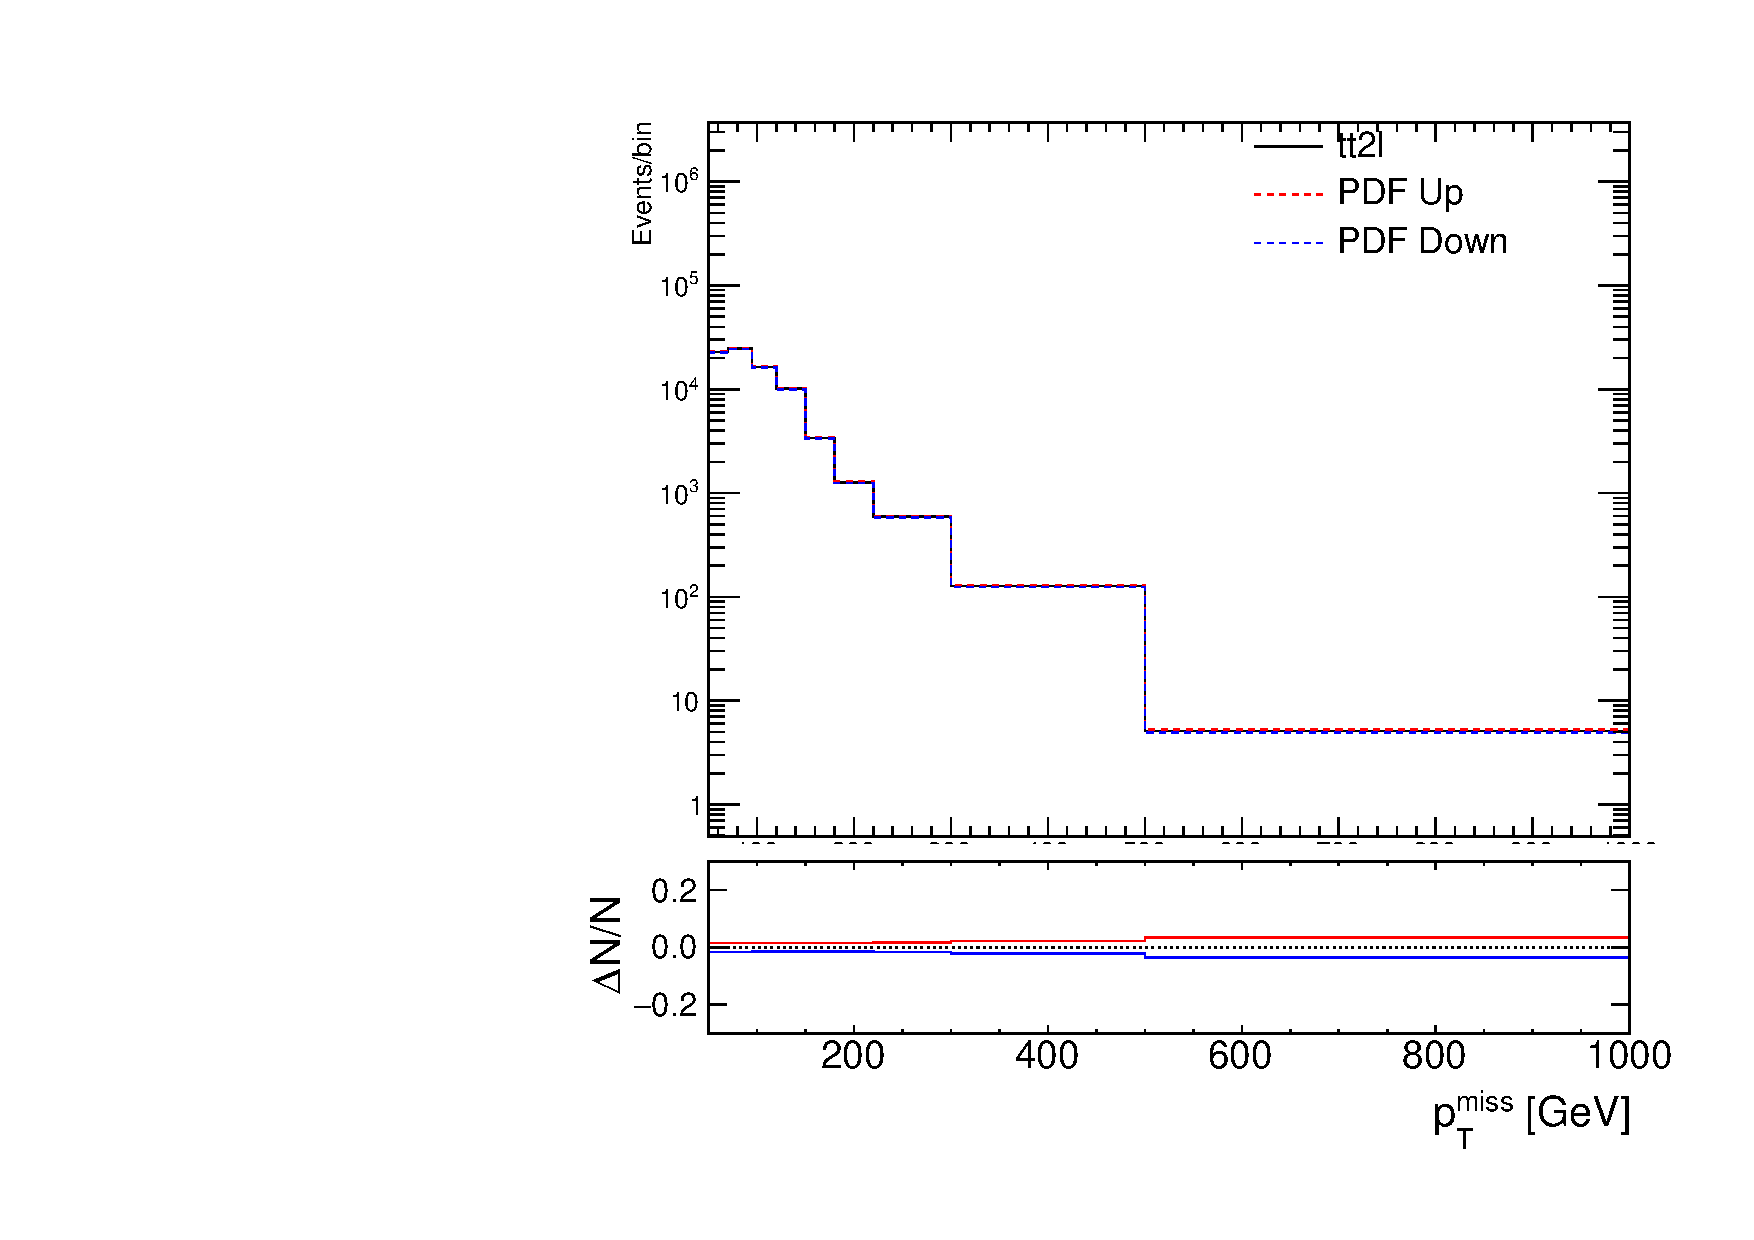
\includegraphics[width=0.48\textwidth]{systs/shapes_ttdm805101_sf_lo/tt2l_pdf}}
  \subfloat[][\ttll, low \mttll-OF]{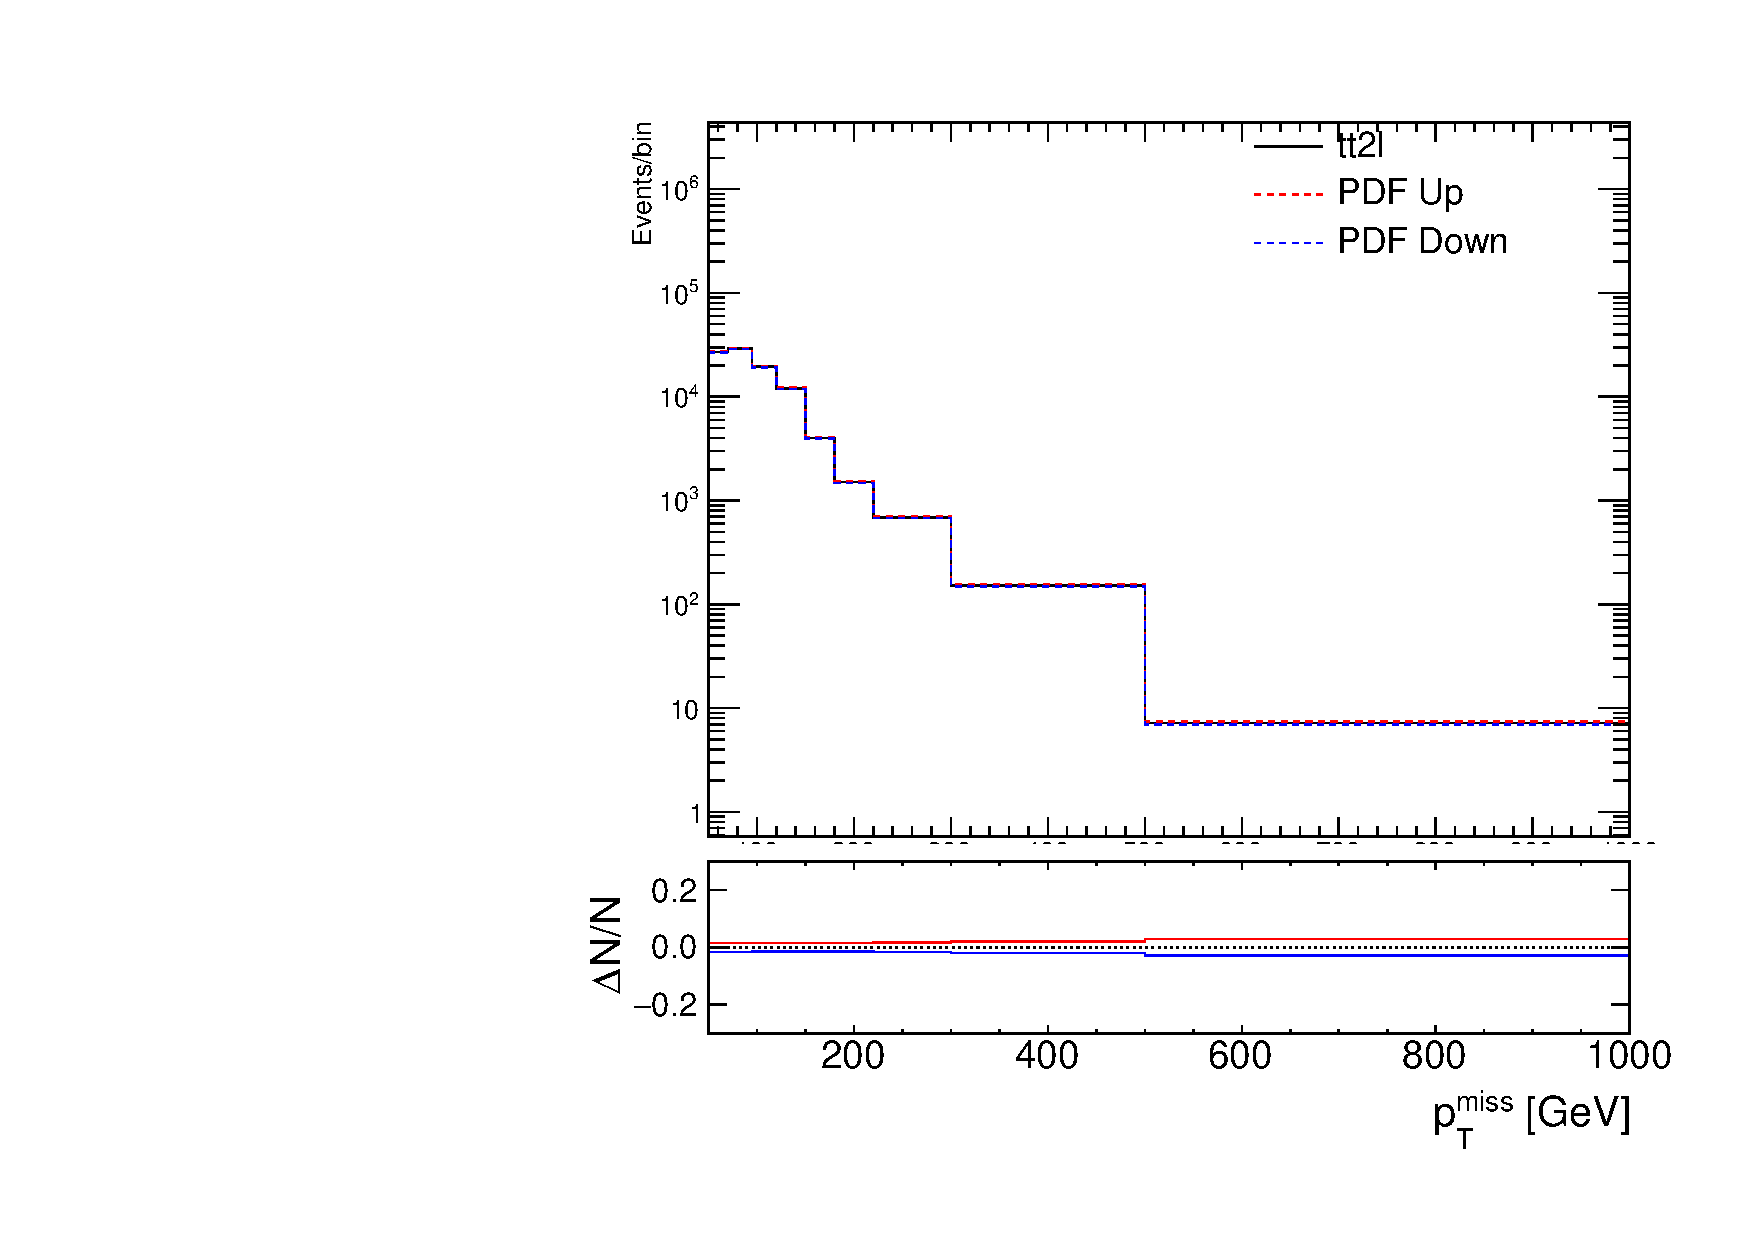
\includegraphics[width=0.48\textwidth]{systs/shapes_ttdm805101_em_lo/tt2l_pdf}} \\
  \subfloat[][\ttll, high \mttll-SF]{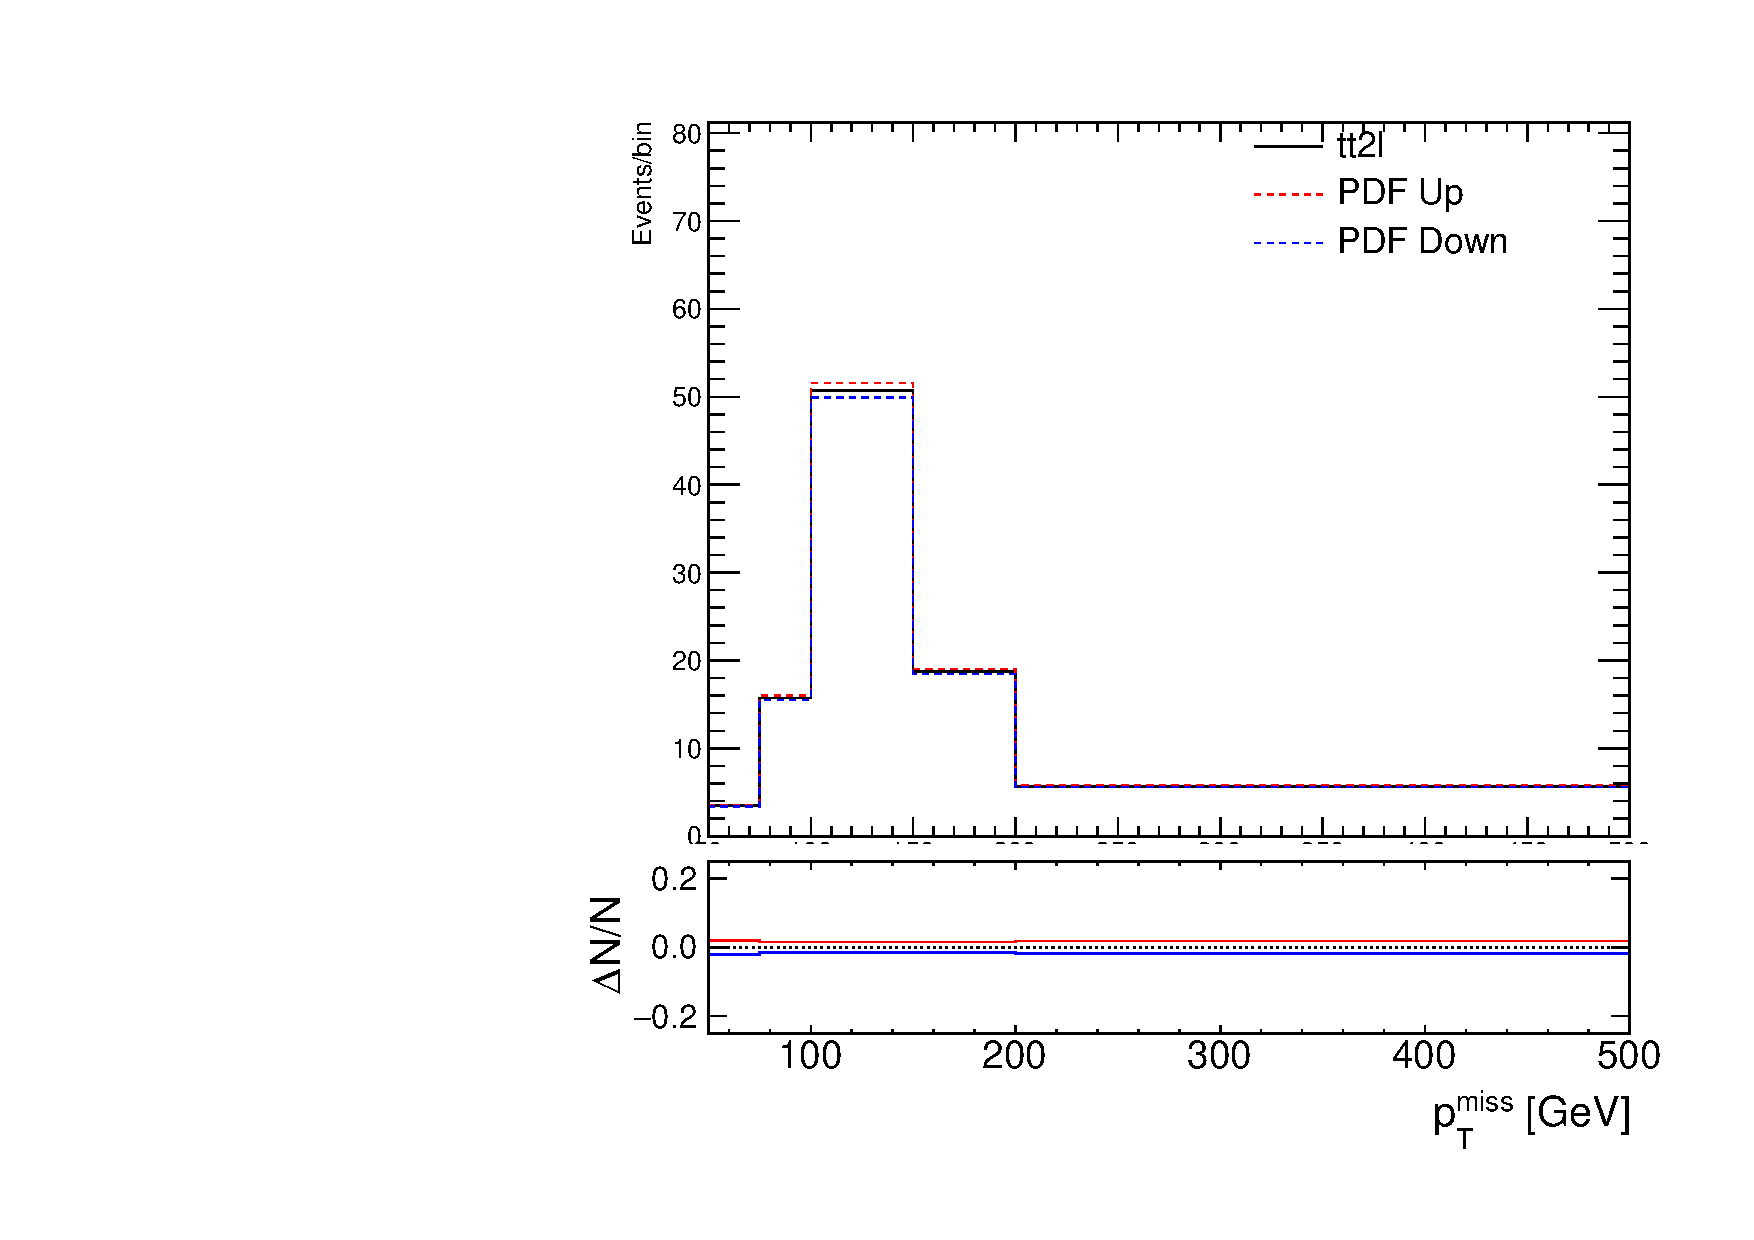
\includegraphics[width=0.48\textwidth]{systs/shapes_ttdm805101_sf_hi/tt2l_pdf}}
  \subfloat[][\ttll, high \mttll-OF]{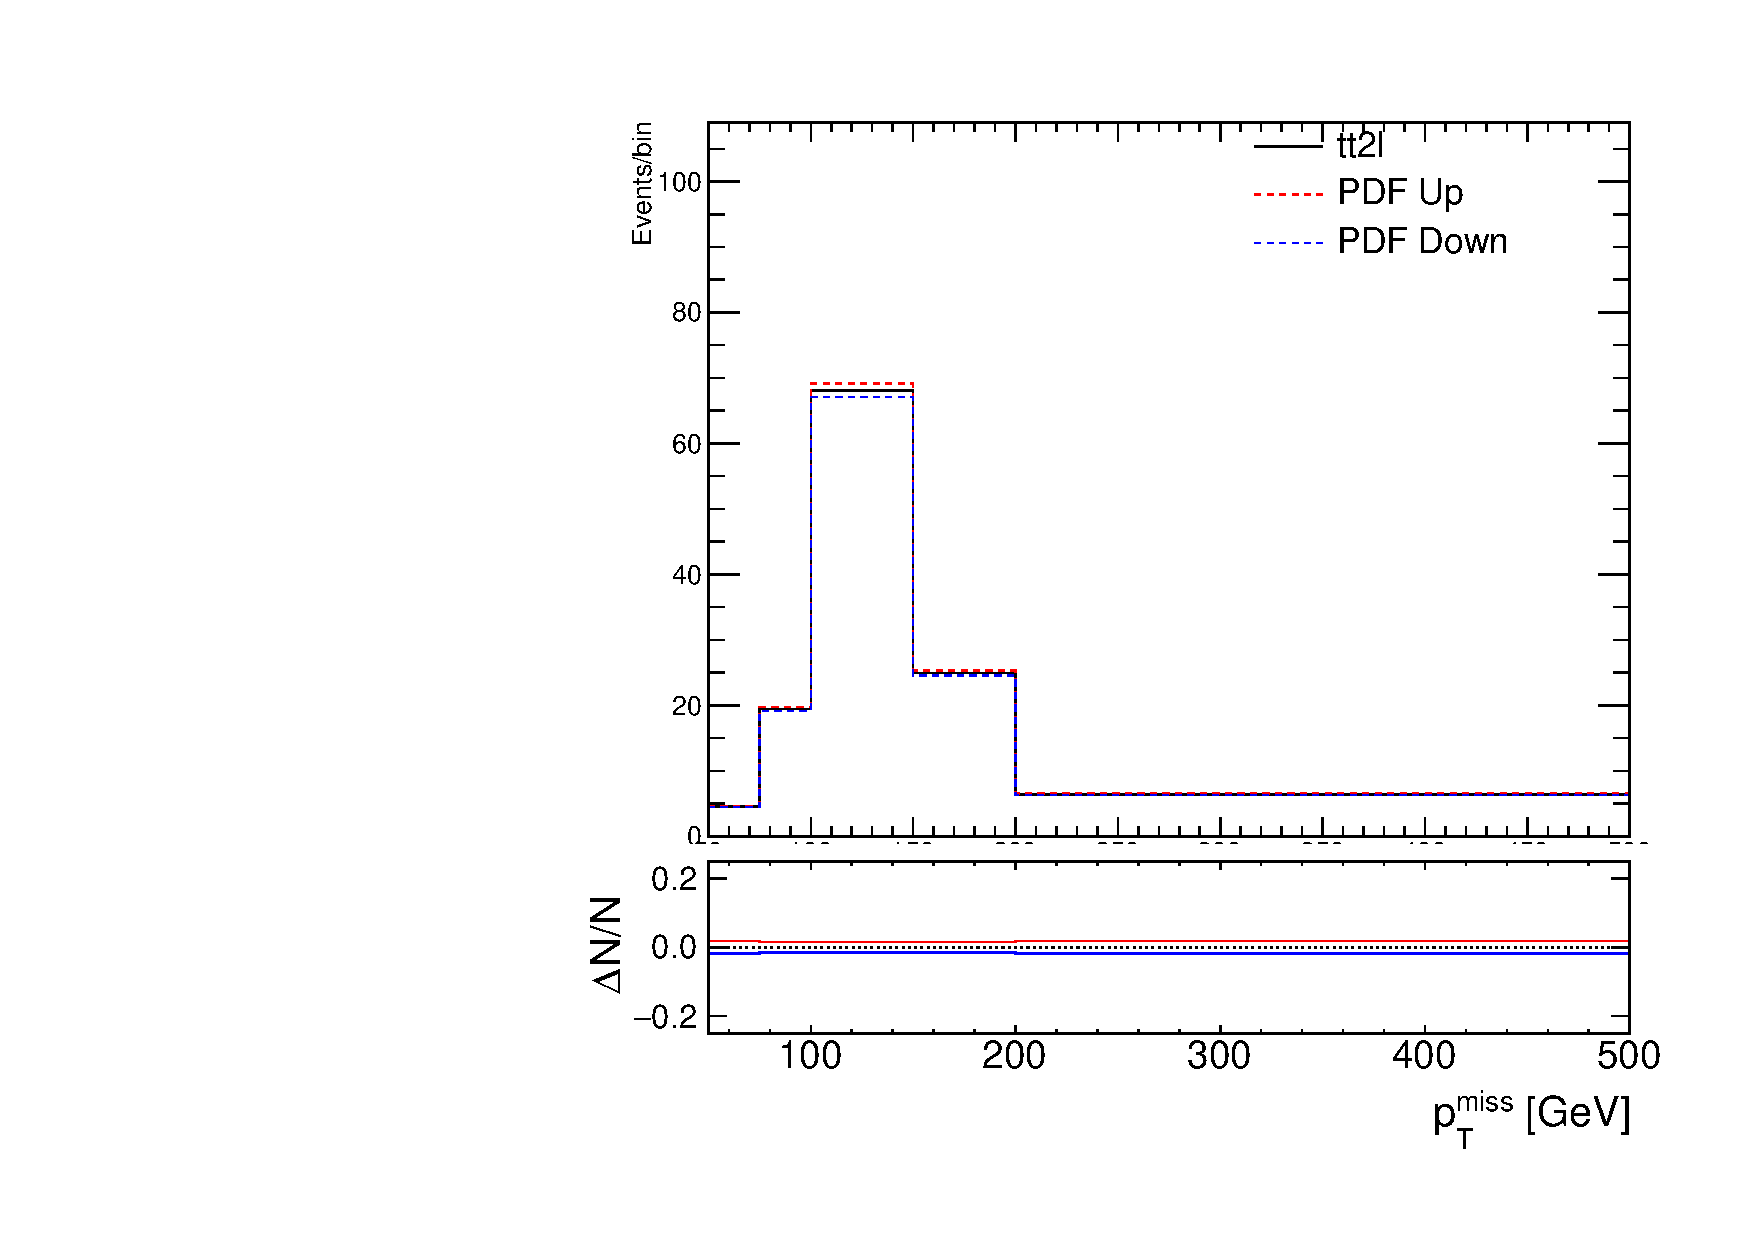
\includegraphics[width=0.48\textwidth]{systs/shapes_ttdm805101_em_hi/tt2l_pdf}}
  \caption{The variation in the \ptmiss spectra for \ttll in the low and high \mttll SRs due to the variation of the pdf uncertainty $+1\sigma$ (red) and $-1\sigma$ (blue). The normalized residuals of the ``up'' and ``down'' shapes are shown in the lower panel.}
  \label{fig:PDFshape}
\end{figure}

\clearpage 

\section{Signal shape systematics: scalar mediated, $\mMed=10\:\GeV$, $\mDM=1\:\GeV$} 
\label{sec:s10syst}

\begin{figure}[h]
  \centering
  \subfloat[][\ttll+\XX, low \mttll-SF]{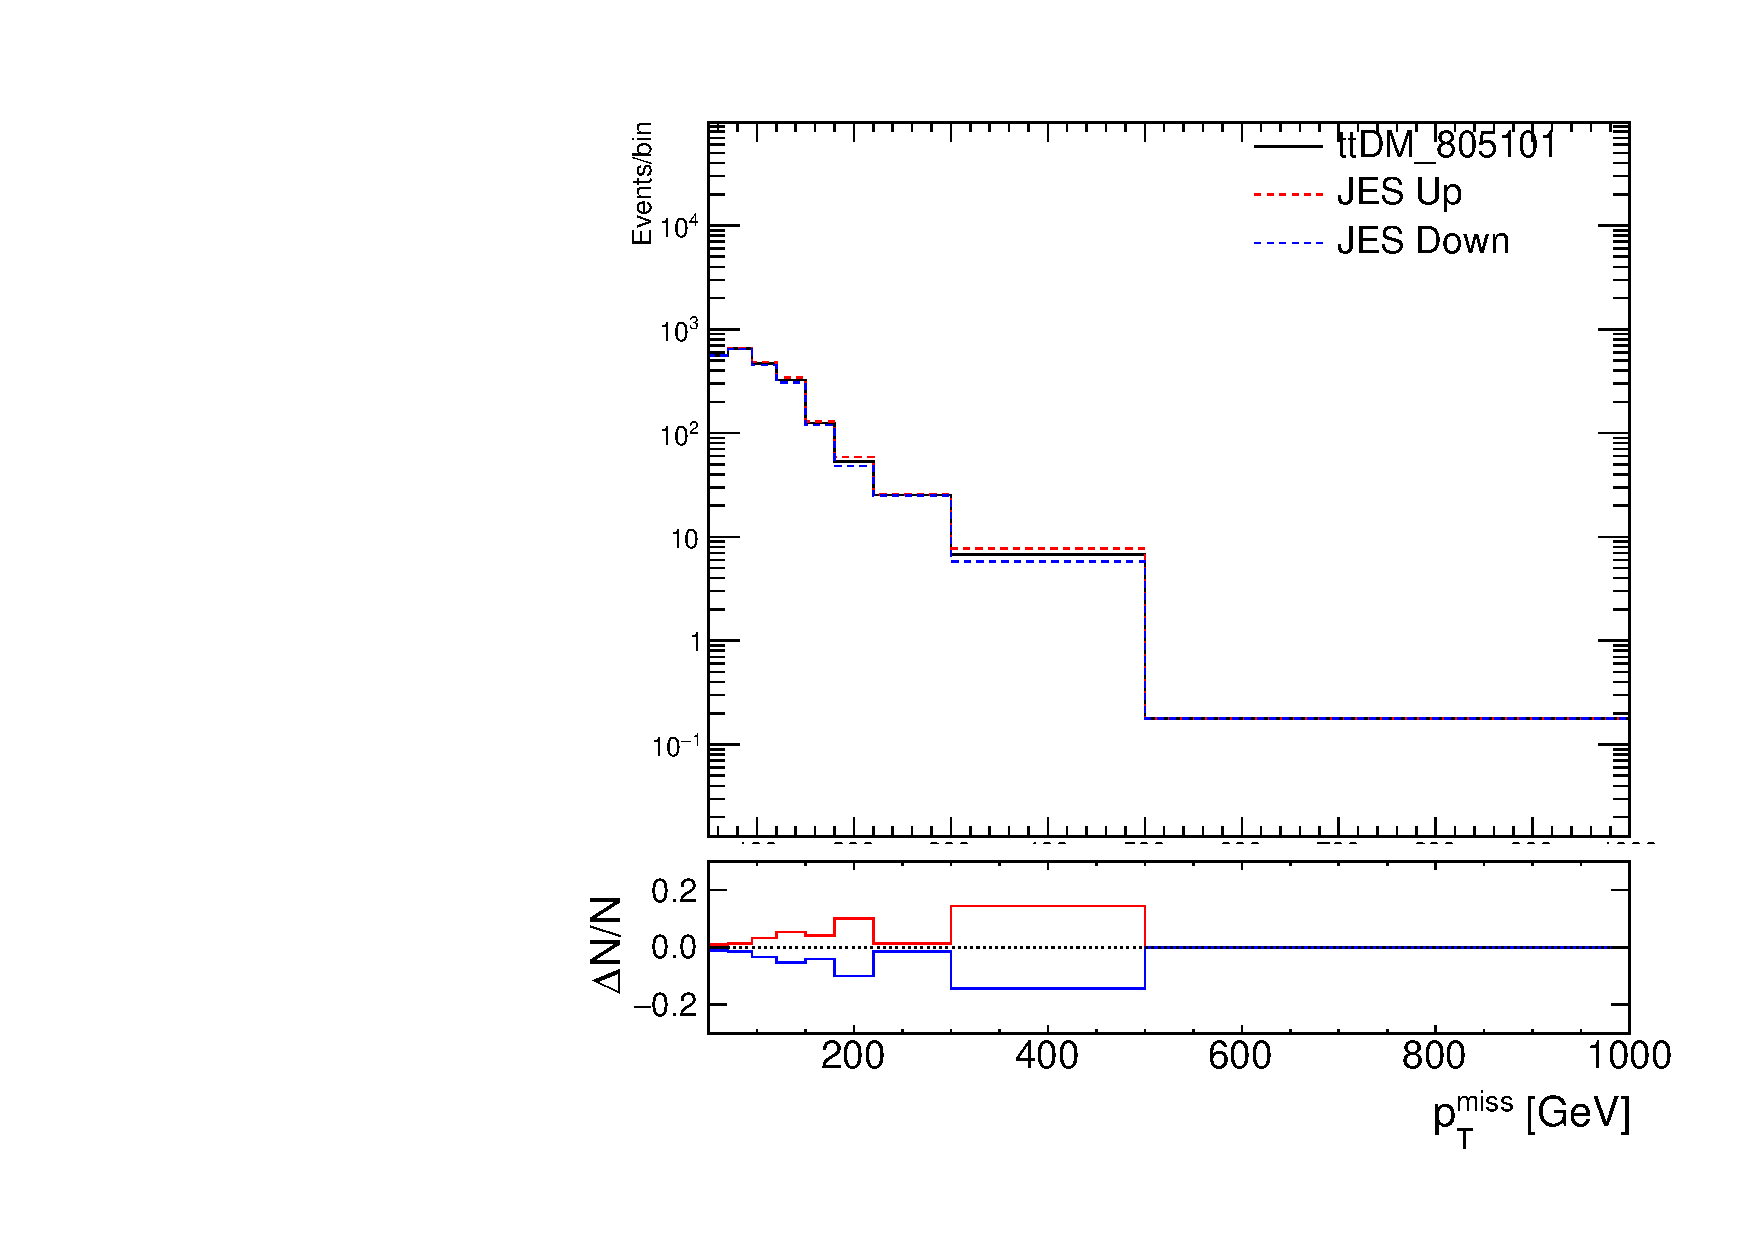
\includegraphics[width=0.48\textwidth]{systs/shapes_ttdm805101_sf_lo/ttDM_805101_CMS_scale_j}}
  \subfloat[][\ttll+\XX, low \mttll-OF]{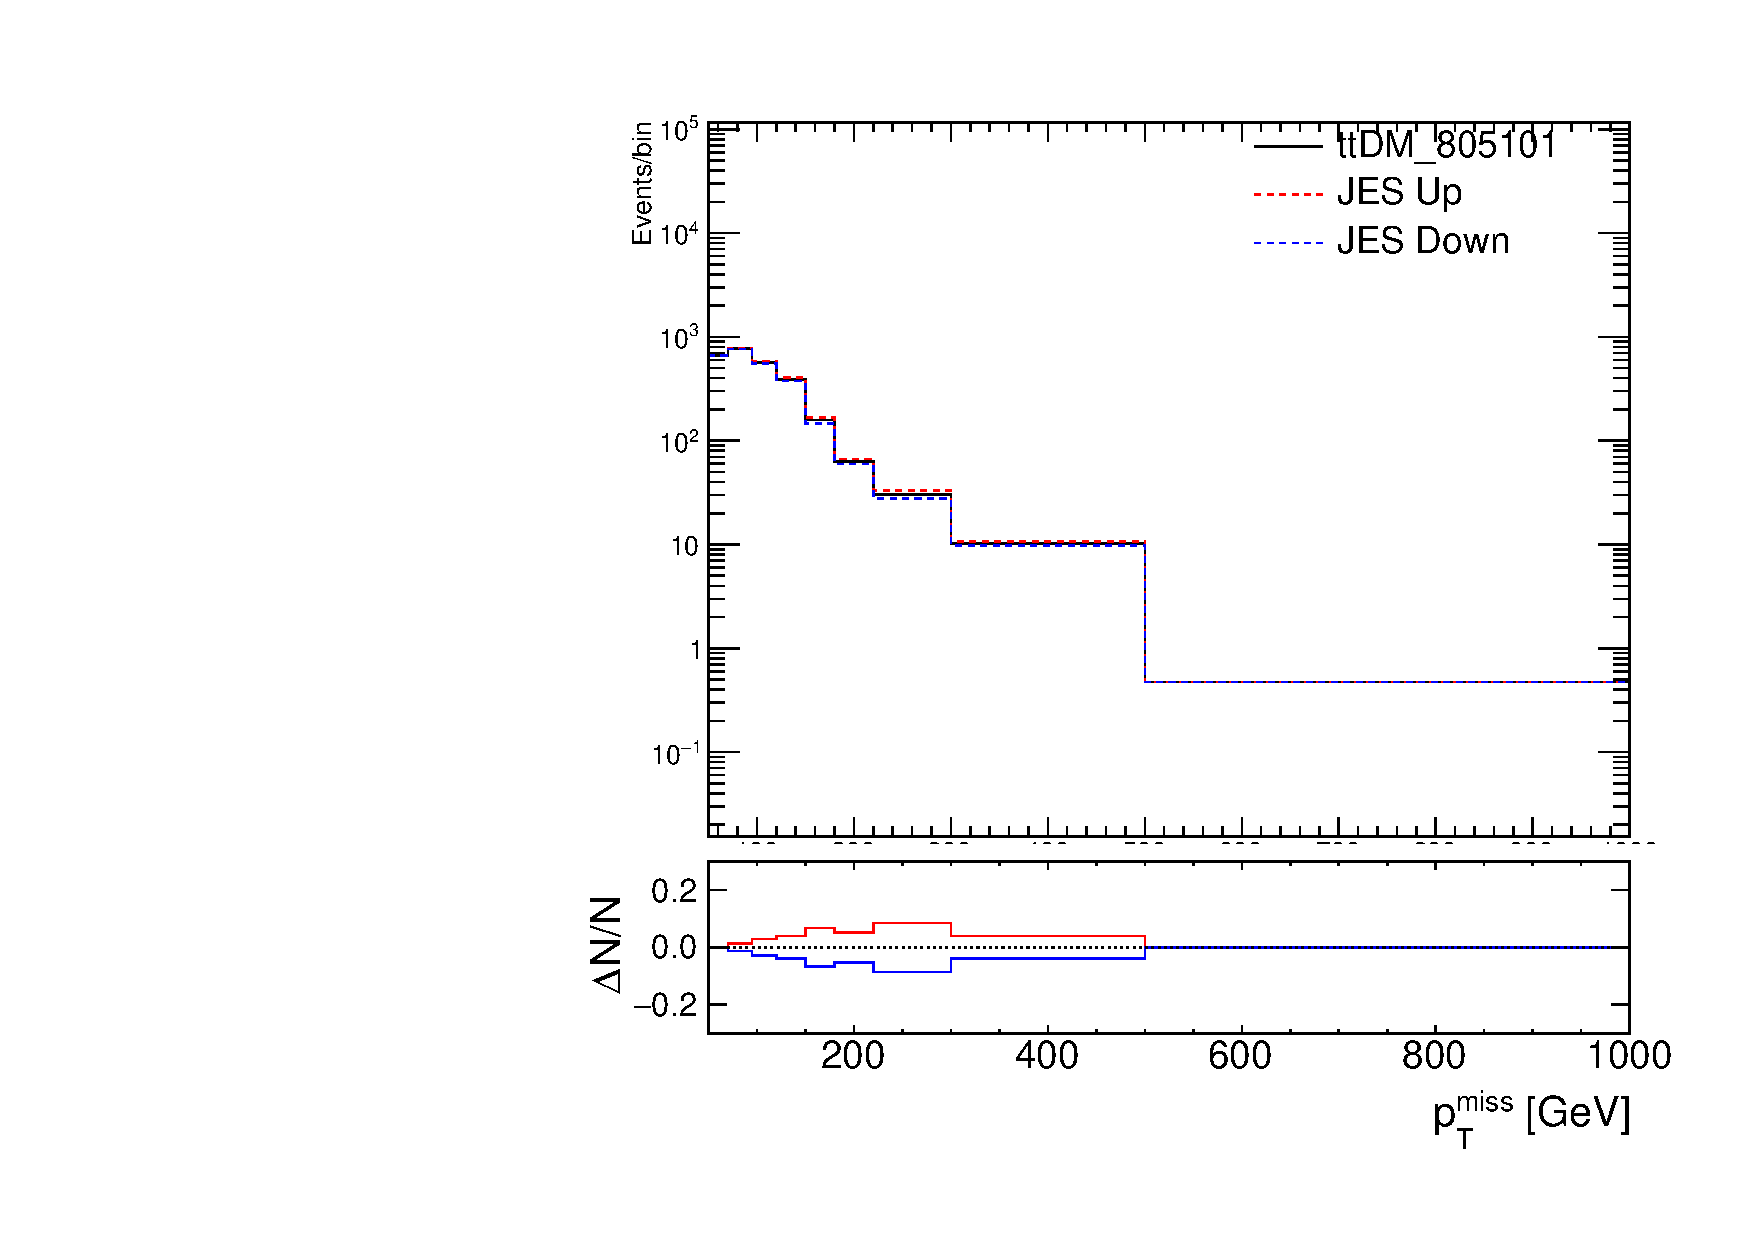
\includegraphics[width=0.48\textwidth]{systs/shapes_ttdm805101_em_lo/ttDM_805101_CMS_scale_j}} \\
  \subfloat[][\ttll+\XX, high \mttll-SF]{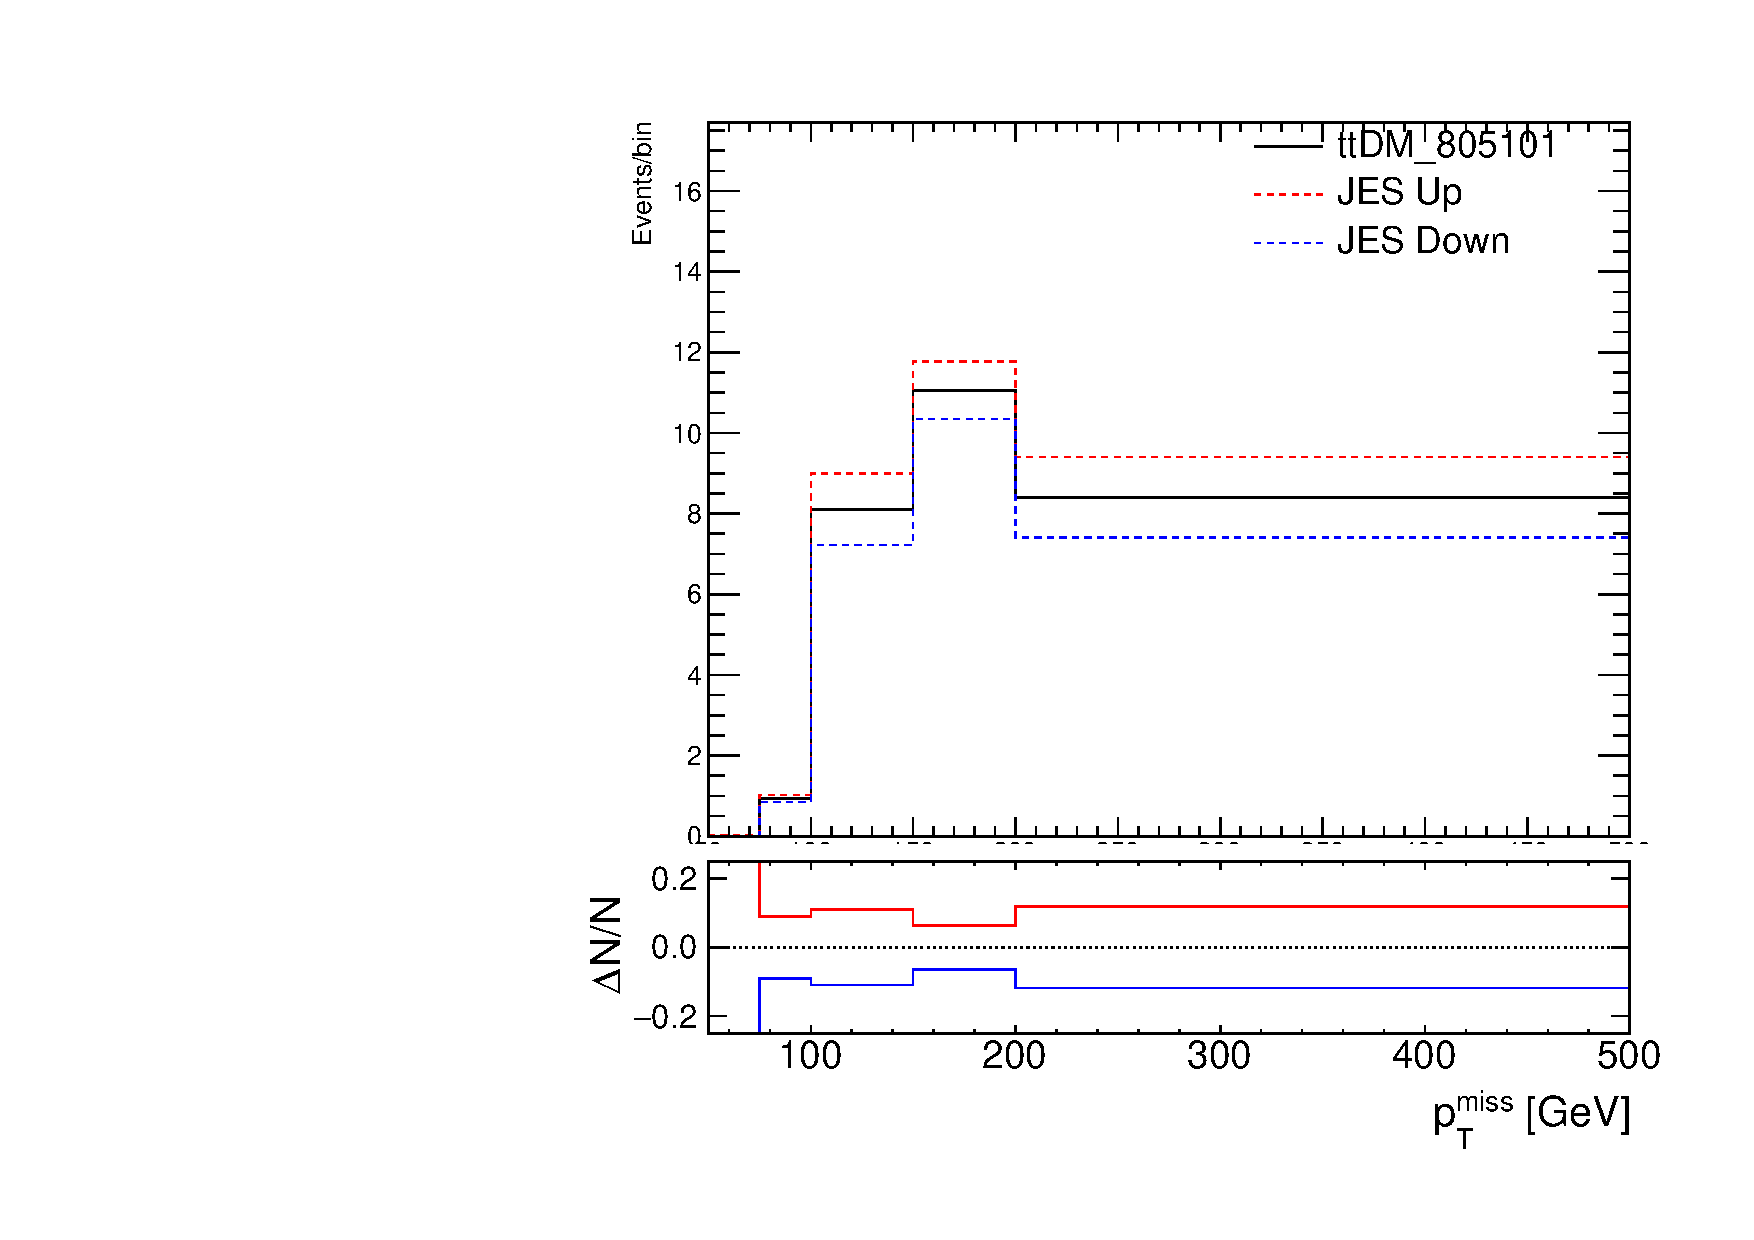
\includegraphics[width=0.48\textwidth]{systs/shapes_ttdm805101_sf_hi/ttDM_805101_CMS_scale_j}}
  \subfloat[][\ttll+\XX, high \mttll-OF]{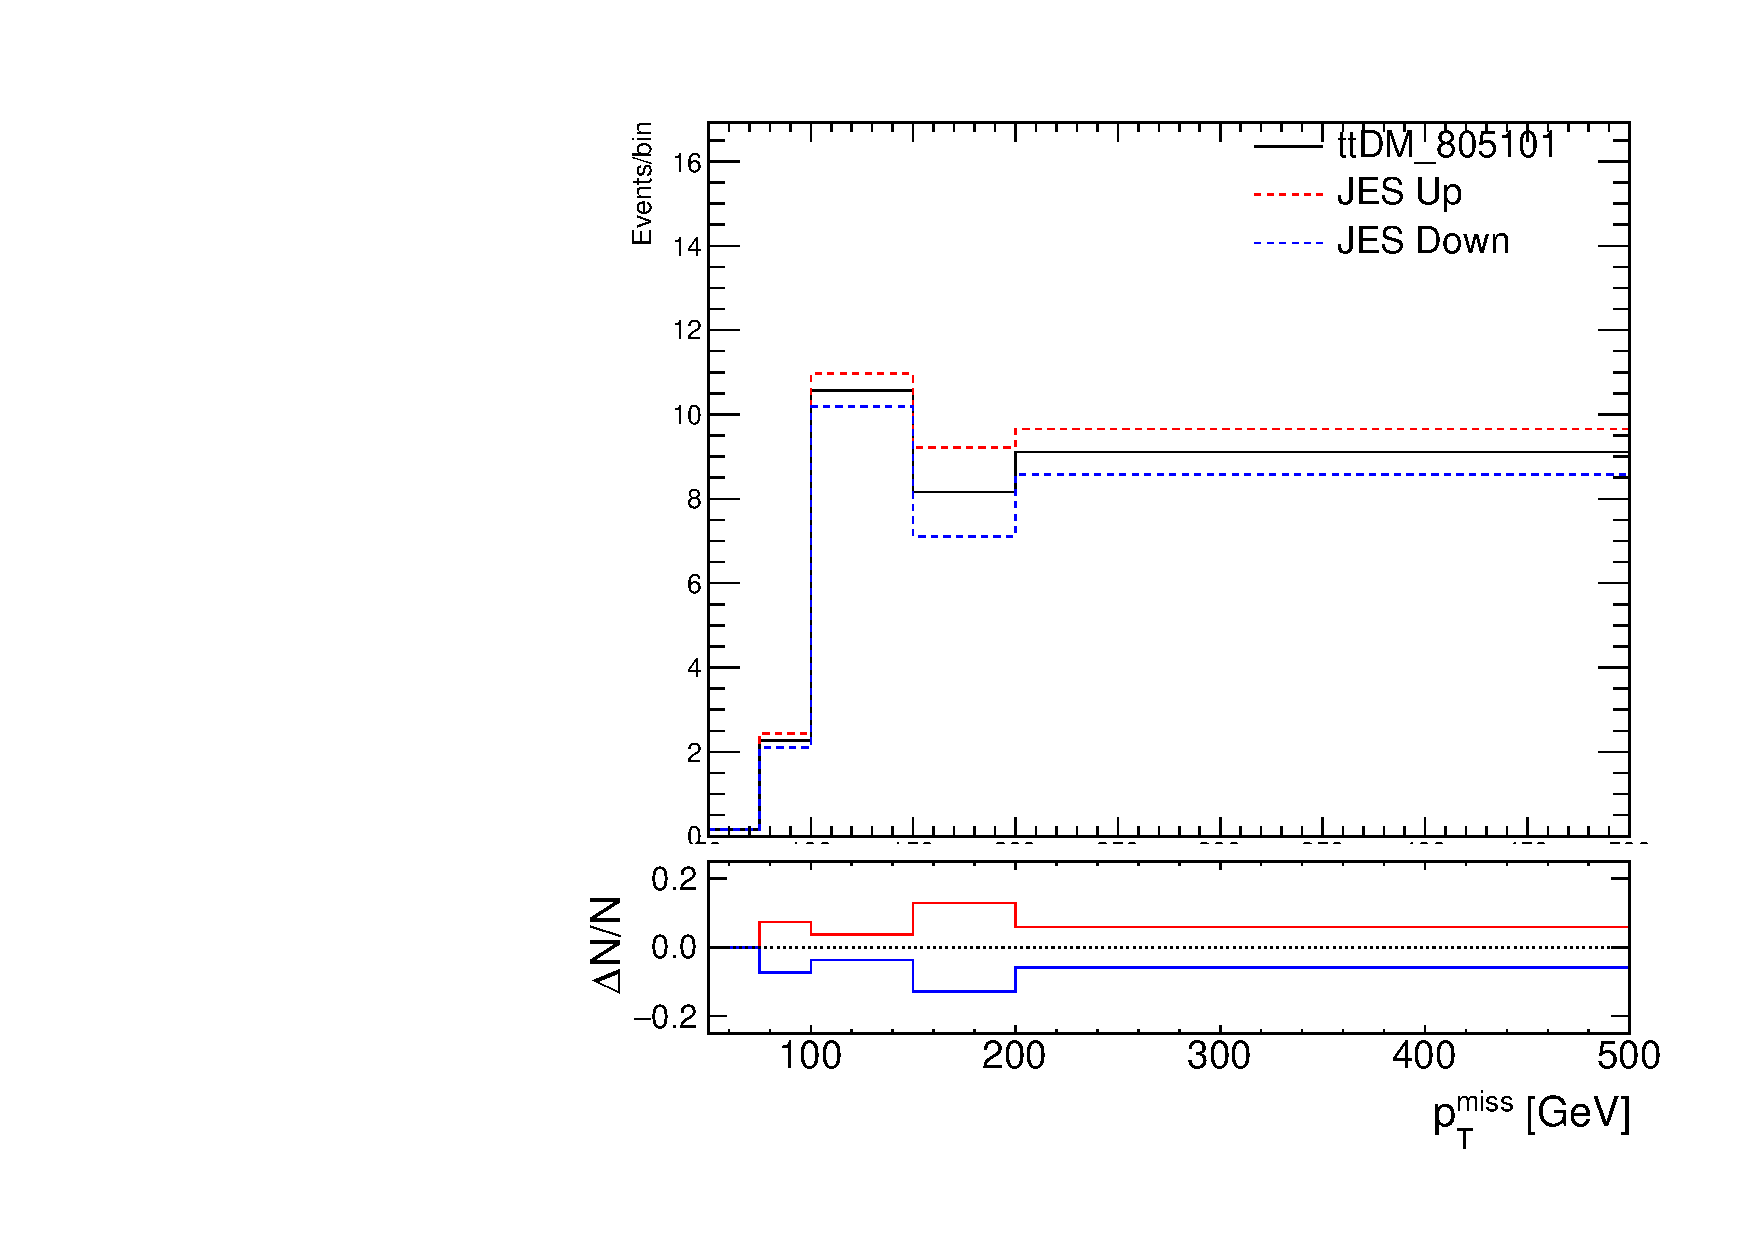
\includegraphics[width=0.48\textwidth]{systs/shapes_ttdm805101_em_hi/ttDM_805101_CMS_scale_j}}
  \caption{The variation in the \ptmiss spectra for a scalar mediated $\mMed=10\:\GeV$ signal with $\mDM=1\:\GeV$ in the low and high \mttll SRs due to the variation of the JES uncertainty by $+1\sigma$ (red) and $-1\sigma$ (blue). The normalized residuals of the ``up'' and ``down'' shapes are shown in the lower panel.}
  \label{fig:JESshape}
\end{figure}

\begin{figure}[h]
  \centering
%  \subfloat[][\ttll+\XX, low \mttll-SF]{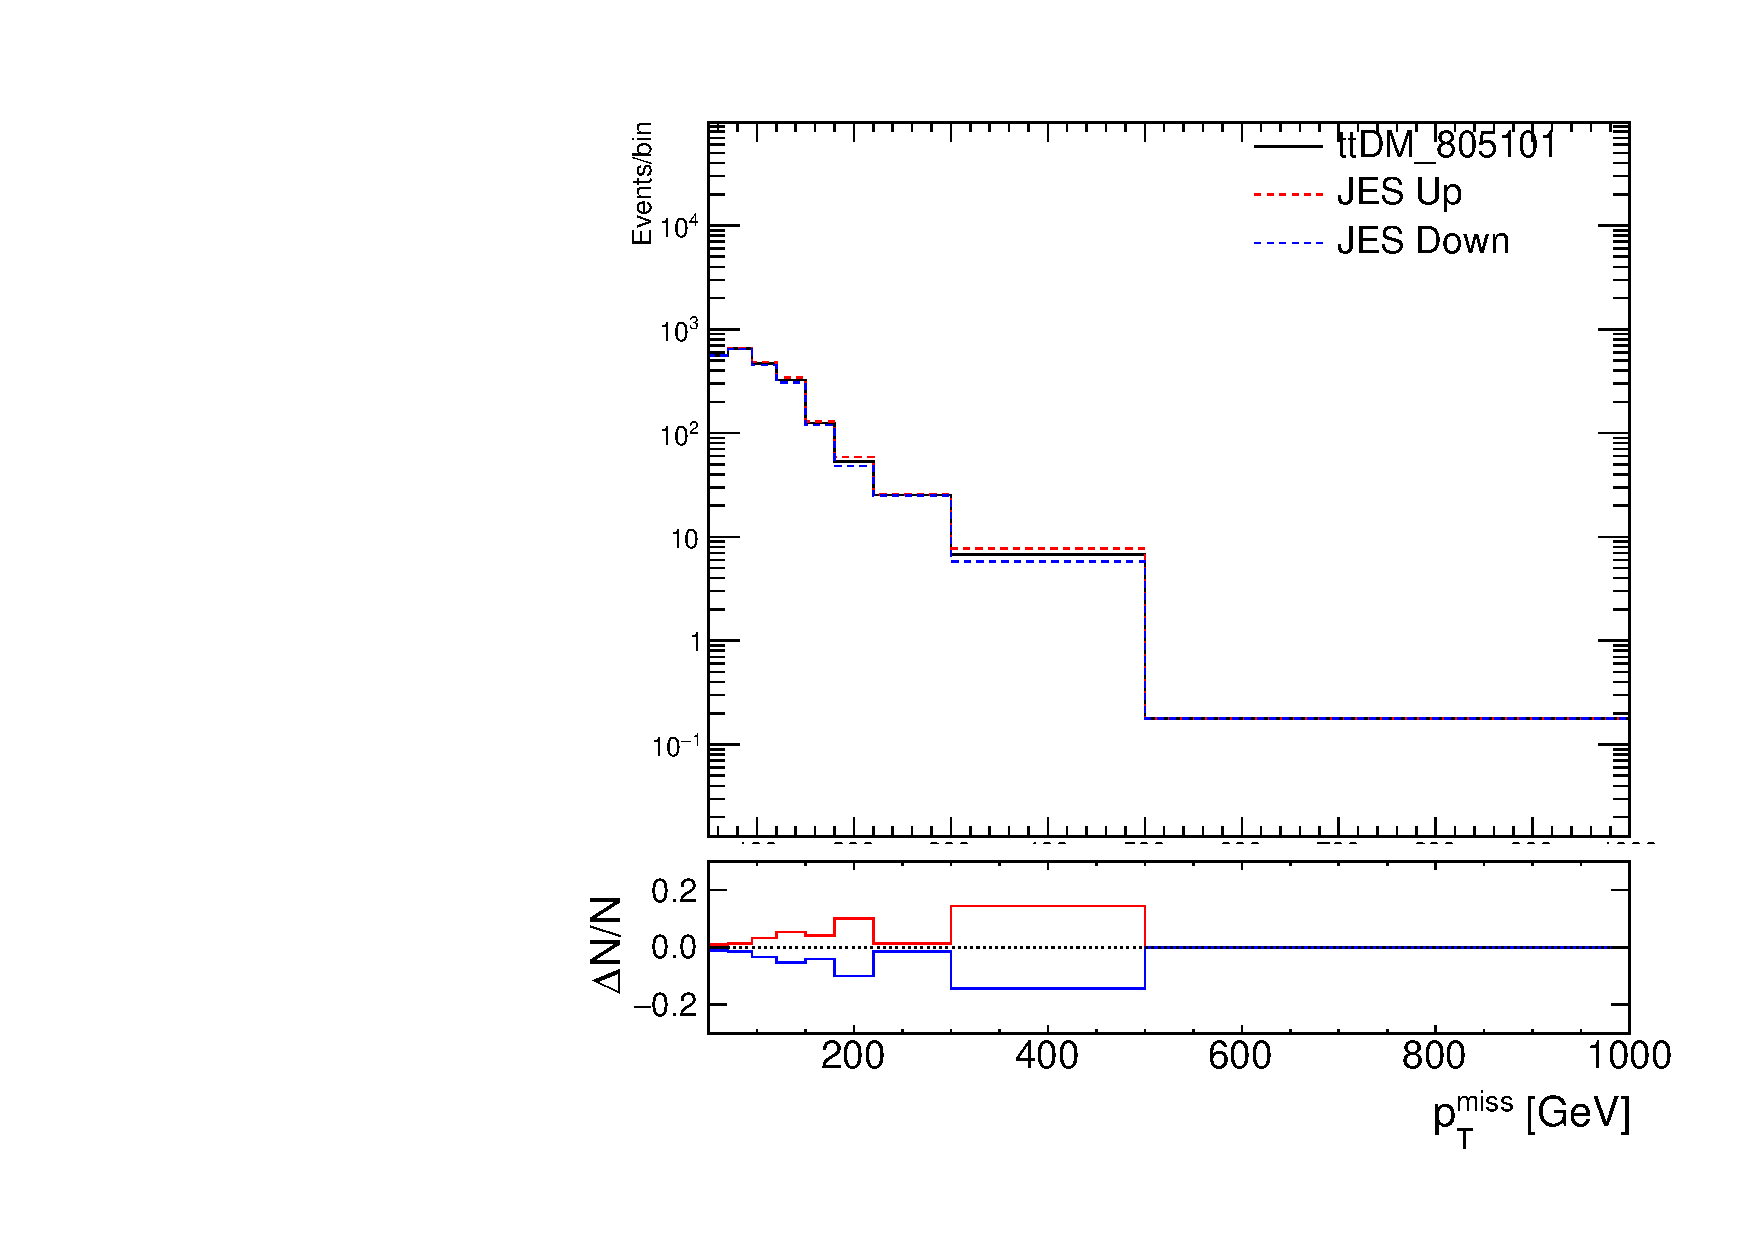
\includegraphics[width=0.48\textwidth]{systs/shapes_ttdm805101_sf_lo/ttDM_805101_CMS_scale_j}}
 % \subfloat[][\ttll+\XX, low \mttll-OF]{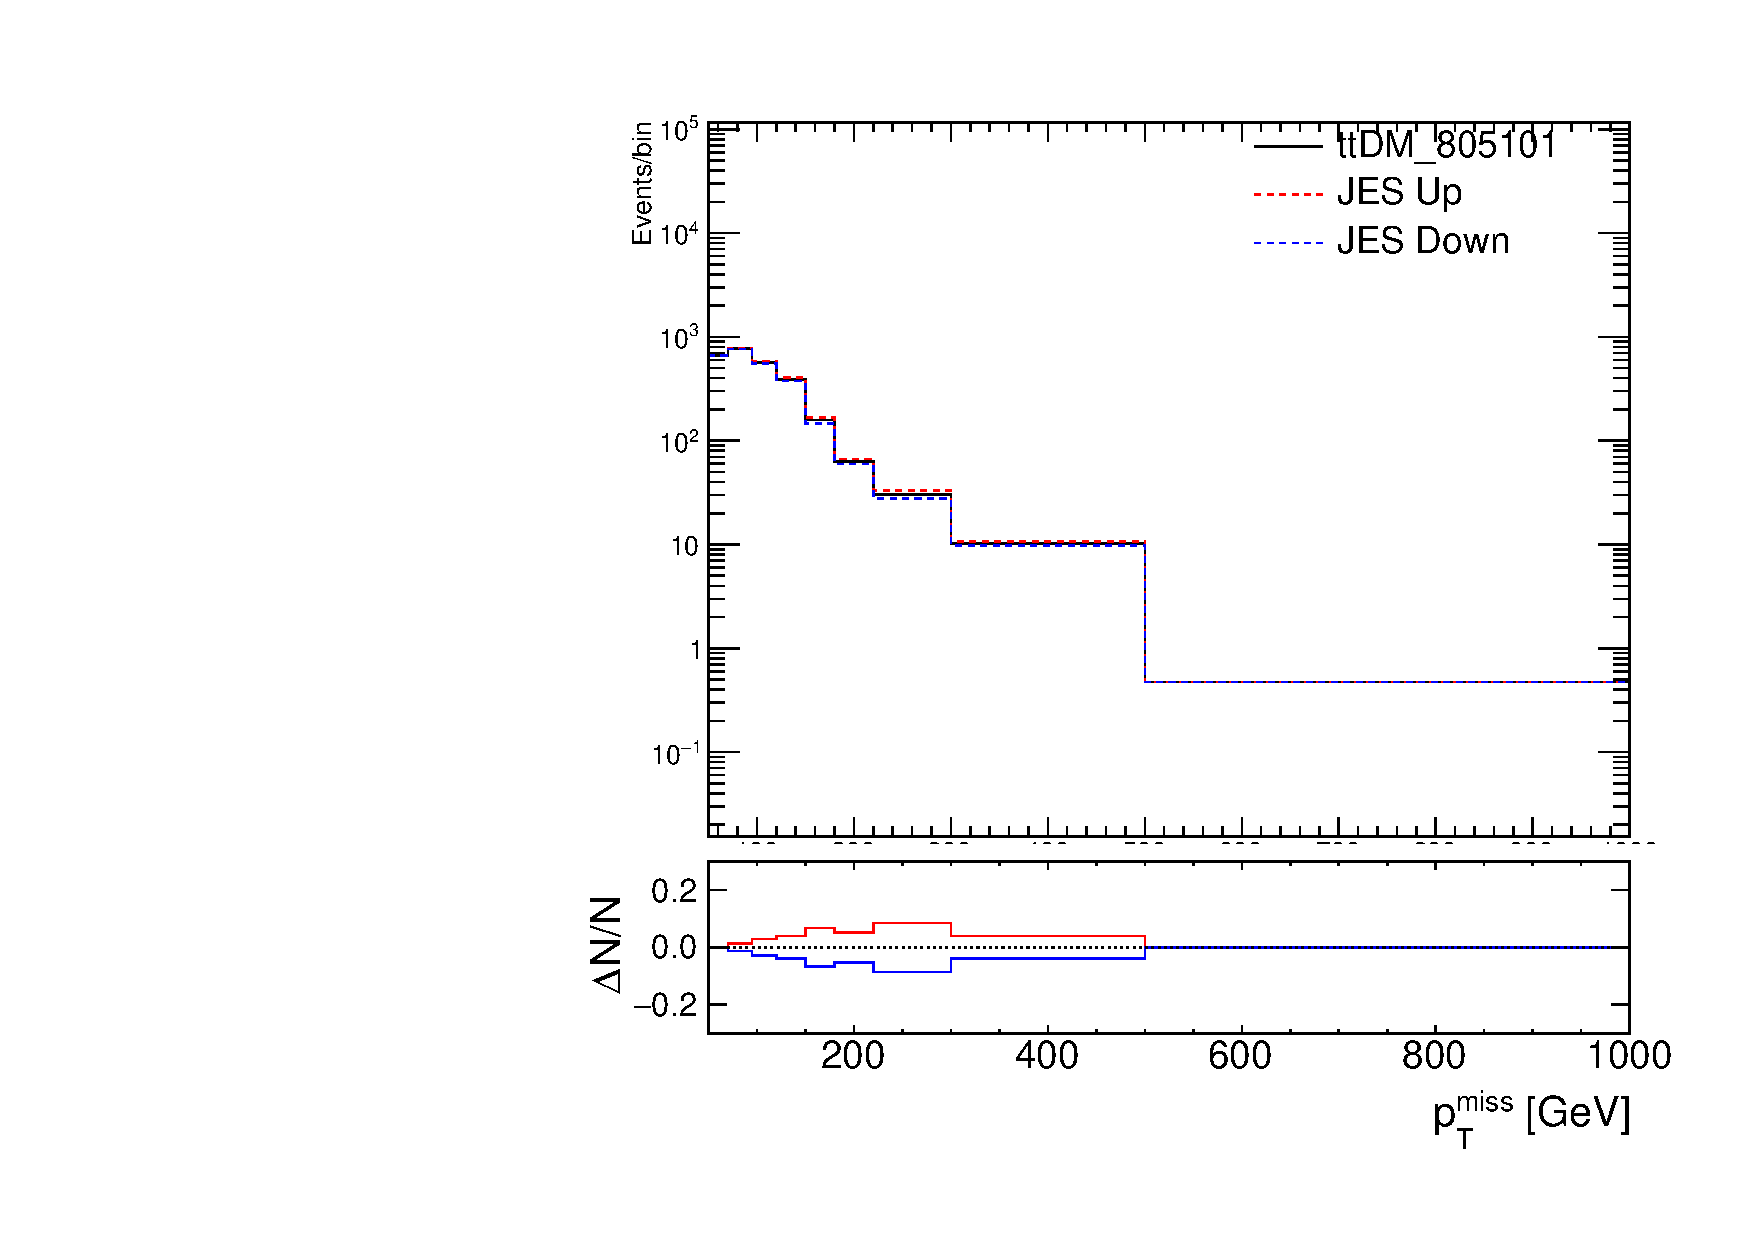
\includegraphics[width=0.48\textwidth]{systs/shapes_ttdm805101_em_lo/ttDM_805101_CMS_scale_j}} \\
  \subfloat[][\ttll+\XX, high \mttll-SF]{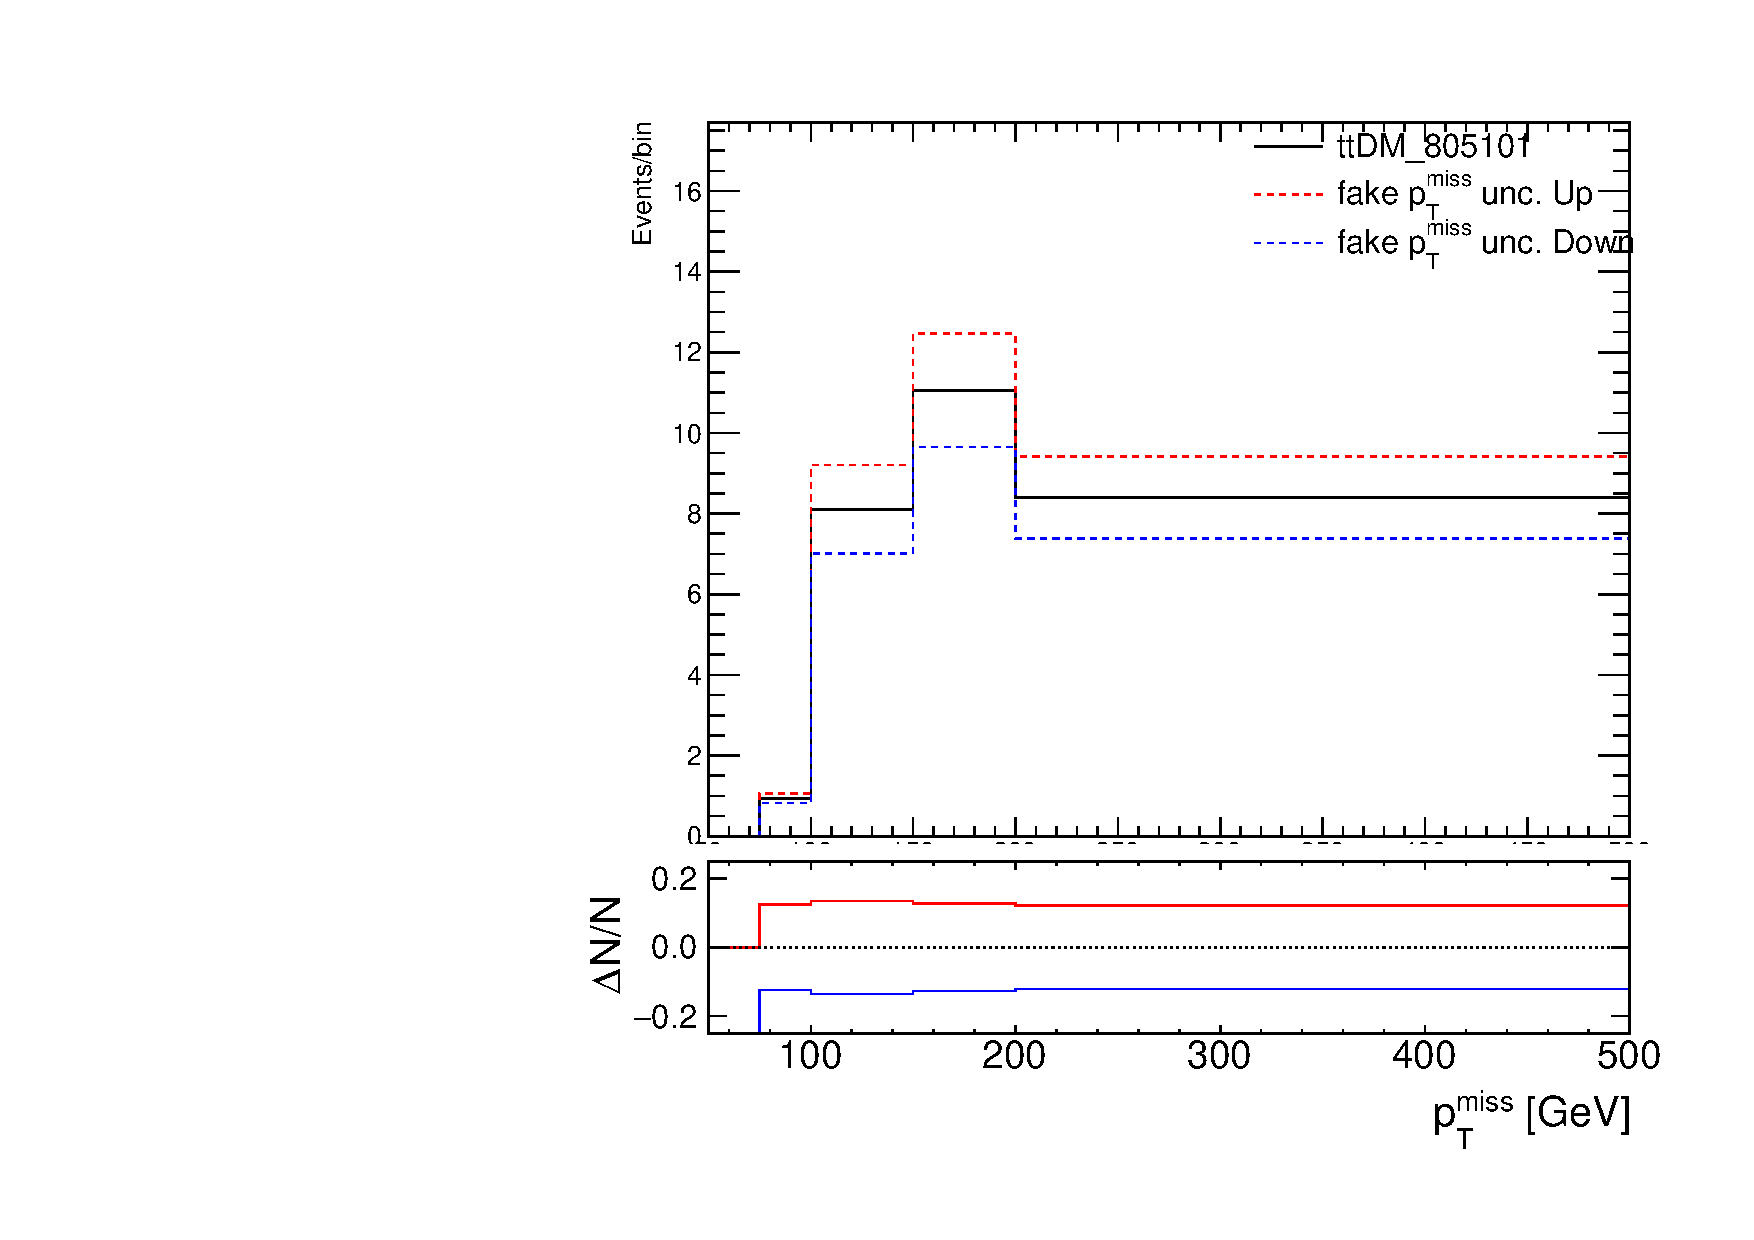
\includegraphics[width=0.48\textwidth]{systs/shapes_ttdm805101_sf_hi/ttDM_805101_RecoilCorr}}
  \subfloat[][\ttll+\XX, high \mttll-OF]{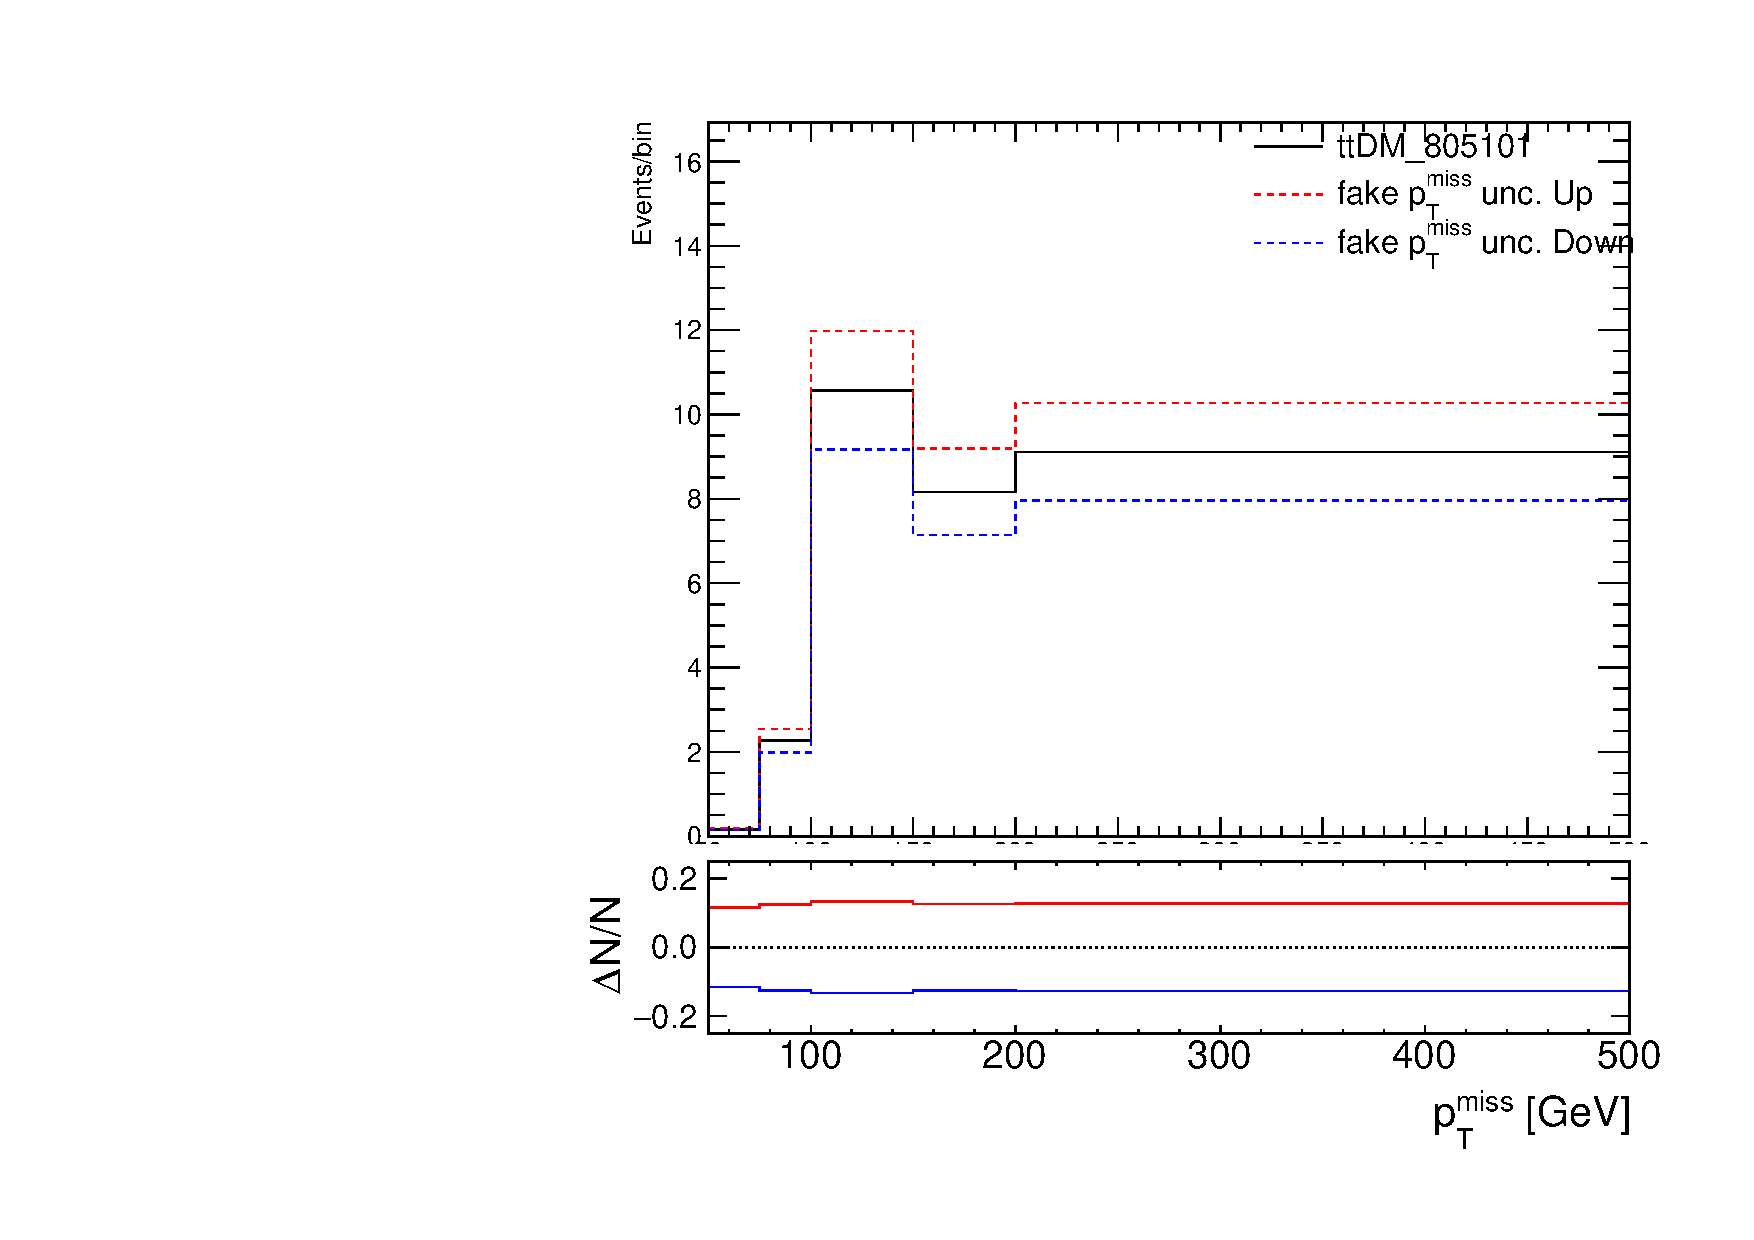
\includegraphics[width=0.48\textwidth]{systs/shapes_ttdm805101_em_hi/ttDM_805101_RecoilCorr}}
  \caption{The variation in the \ptmiss spectra for scalar mediated $\mMed=10\:\GeV$ signal with $\mDM=1\:\GeV$ in the high \mttll SRs due to the variation of the fake \ptmiss uncertainty by $+1\sigma$ (red) and $-1\sigma$ (blue). The normalized residuals of the ``up'' and ``down'' shapes are shown in the lower panel.}
  \label{fig:fakeMETshape}
\end{figure}

\begin{figure}[h]
  \centering
  \subfloat[][\ttll+\XX, low \mttll-SF]{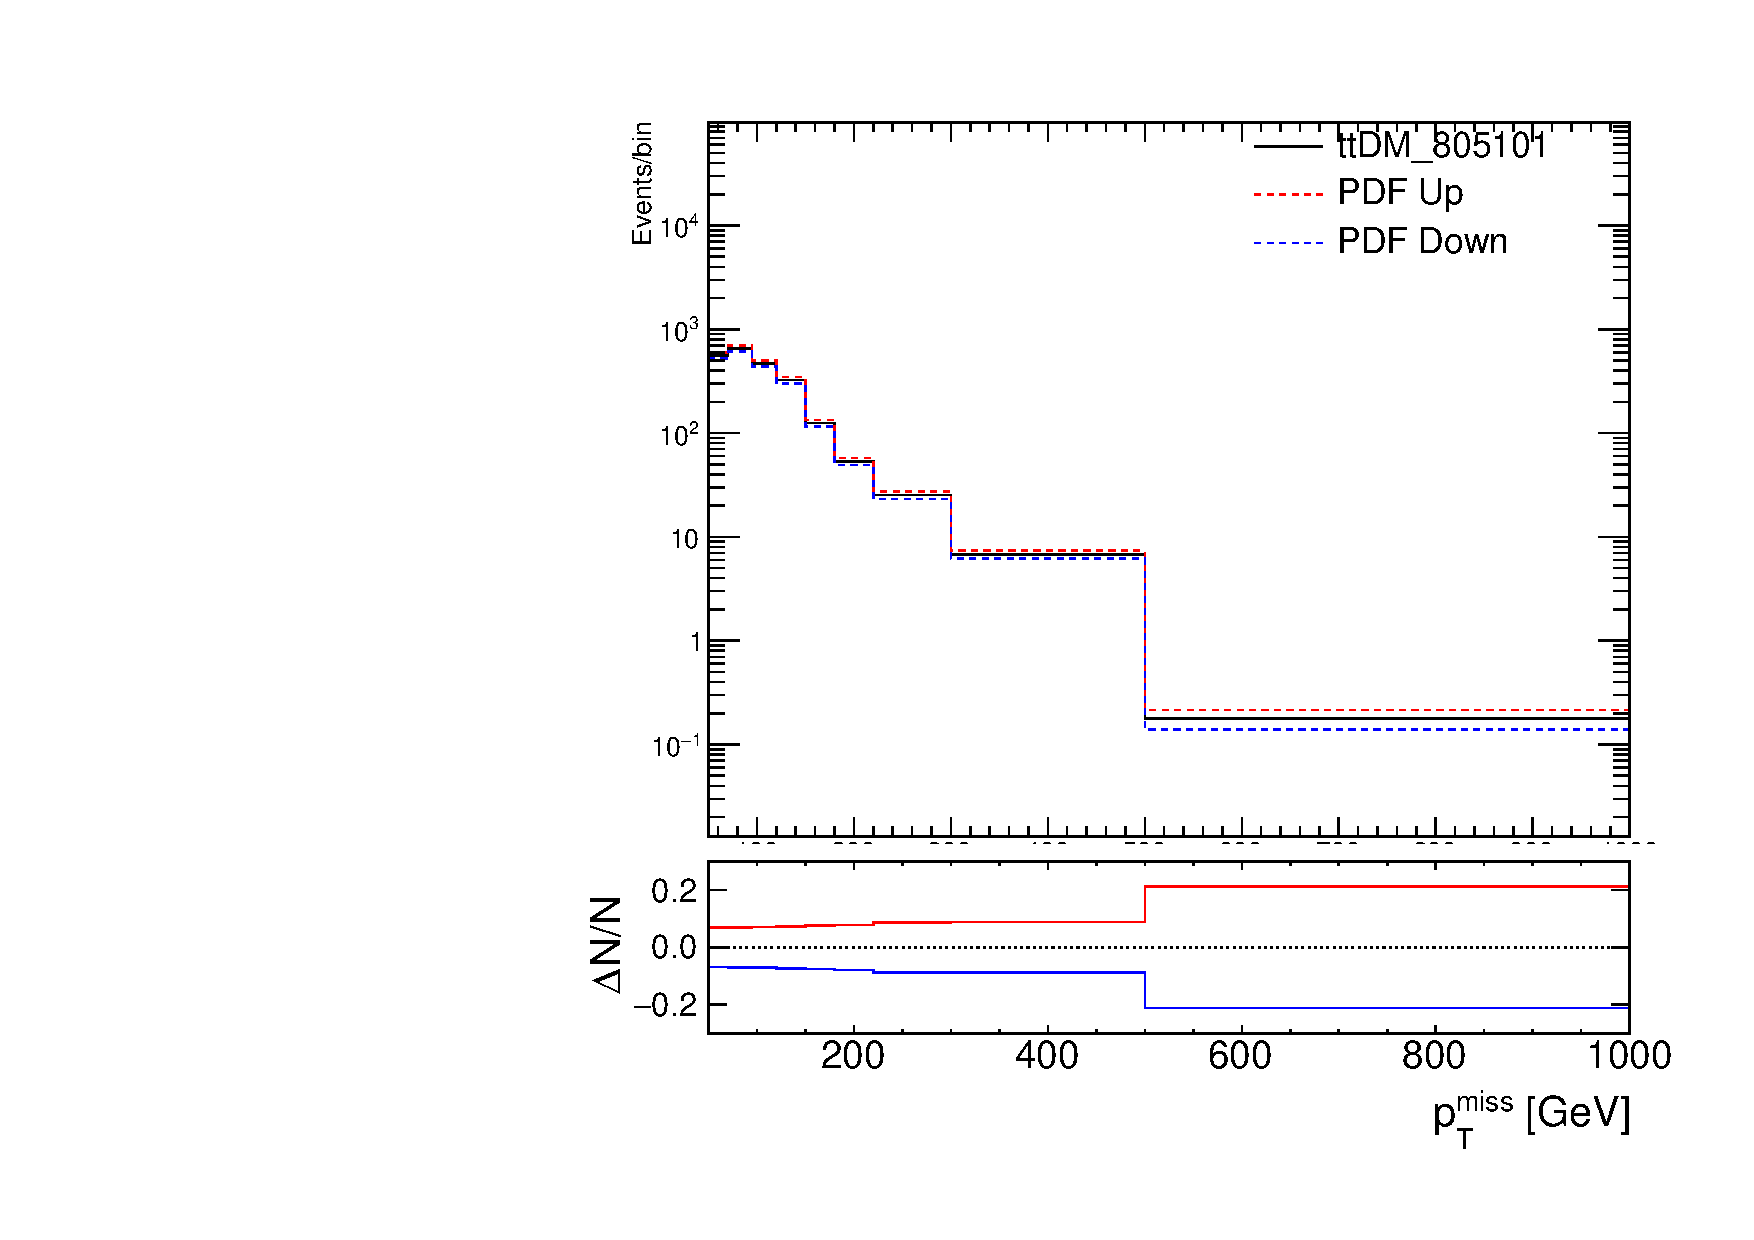
\includegraphics[width=0.48\textwidth]{systs/shapes_ttdm805101_sf_lo/ttDM_805101_pdf}}
  \subfloat[][\ttll+\XX, low \mttll-OF]{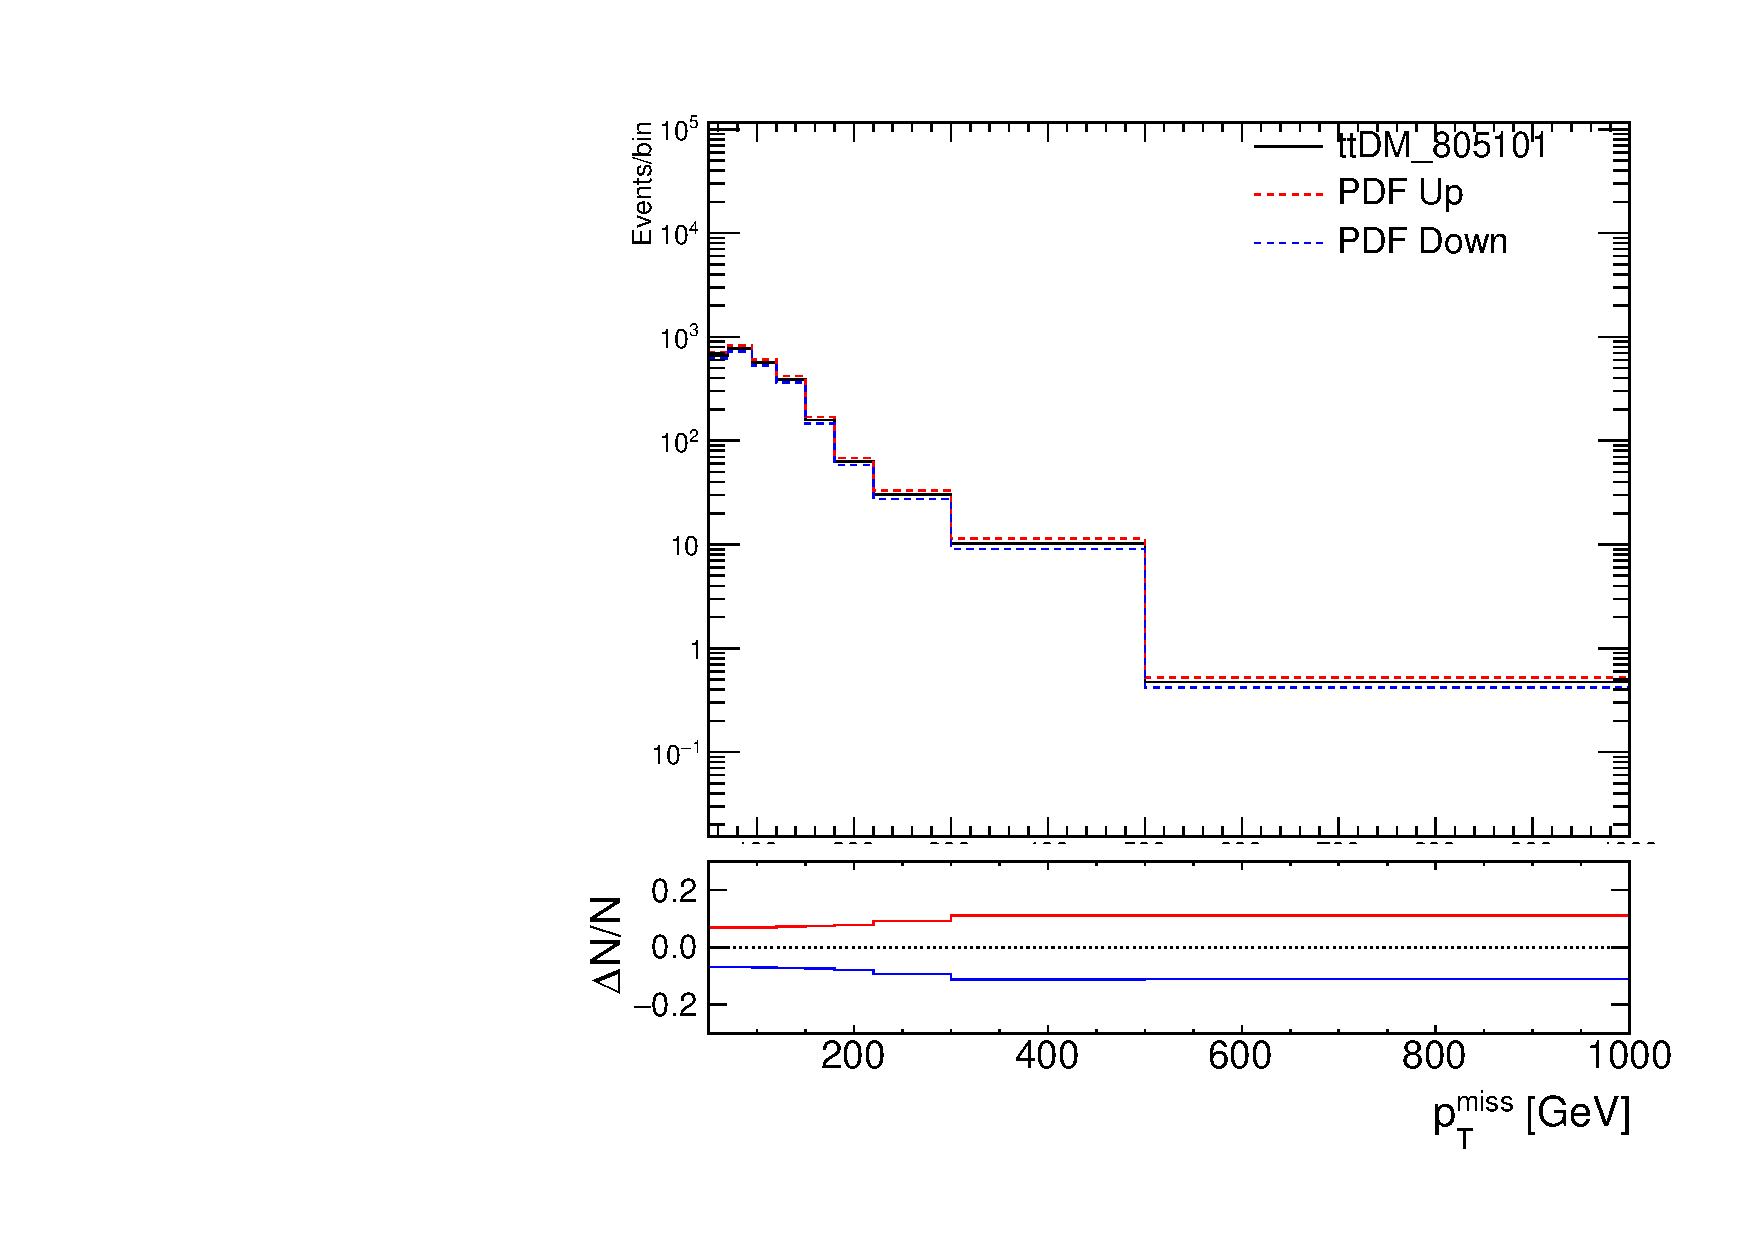
\includegraphics[width=0.48\textwidth]{systs/shapes_ttdm805101_em_lo/ttDM_805101_pdf}} \\
  \subfloat[][\ttll+\XX, high \mttll-SF]{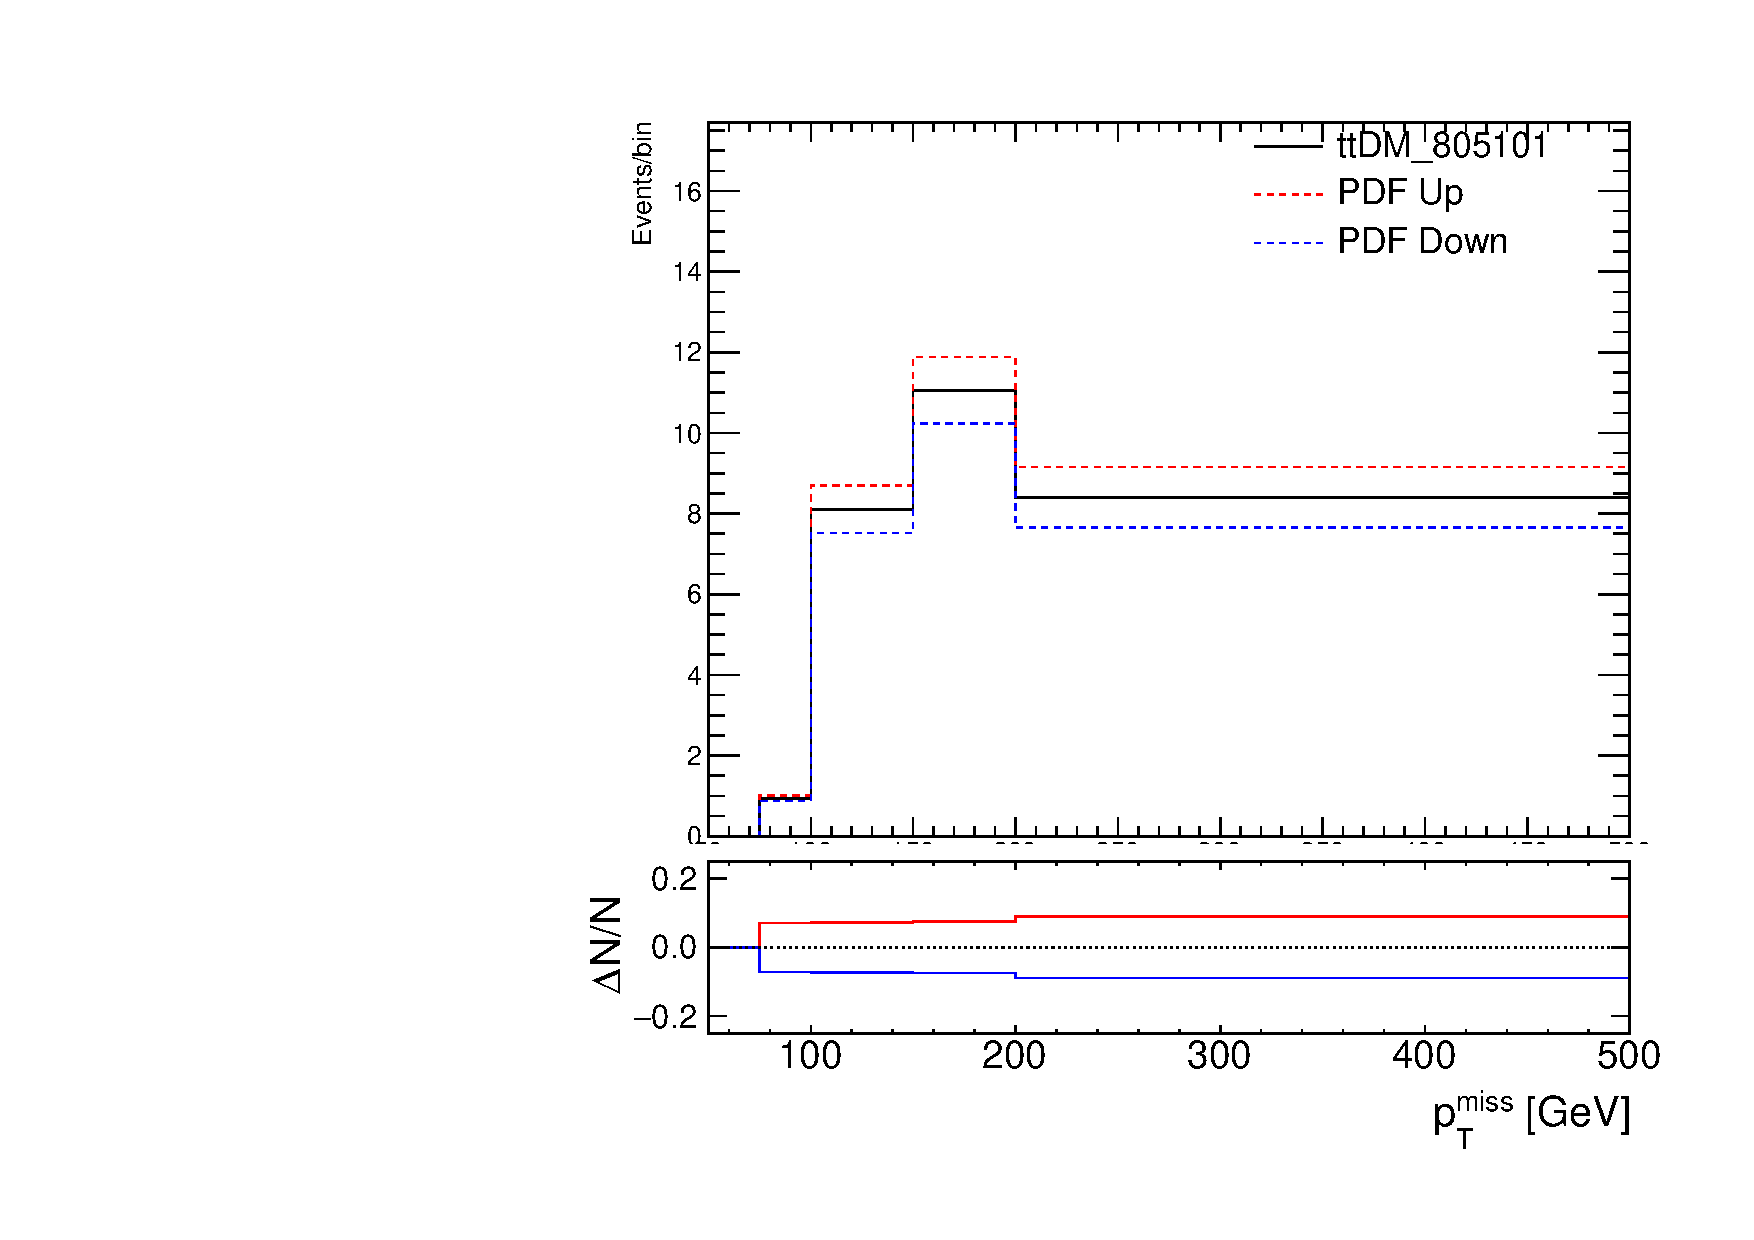
\includegraphics[width=0.48\textwidth]{systs/shapes_ttdm805101_sf_hi/ttDM_805101_pdf}}
  \subfloat[][\ttll+\XX, high \mttll-OF]{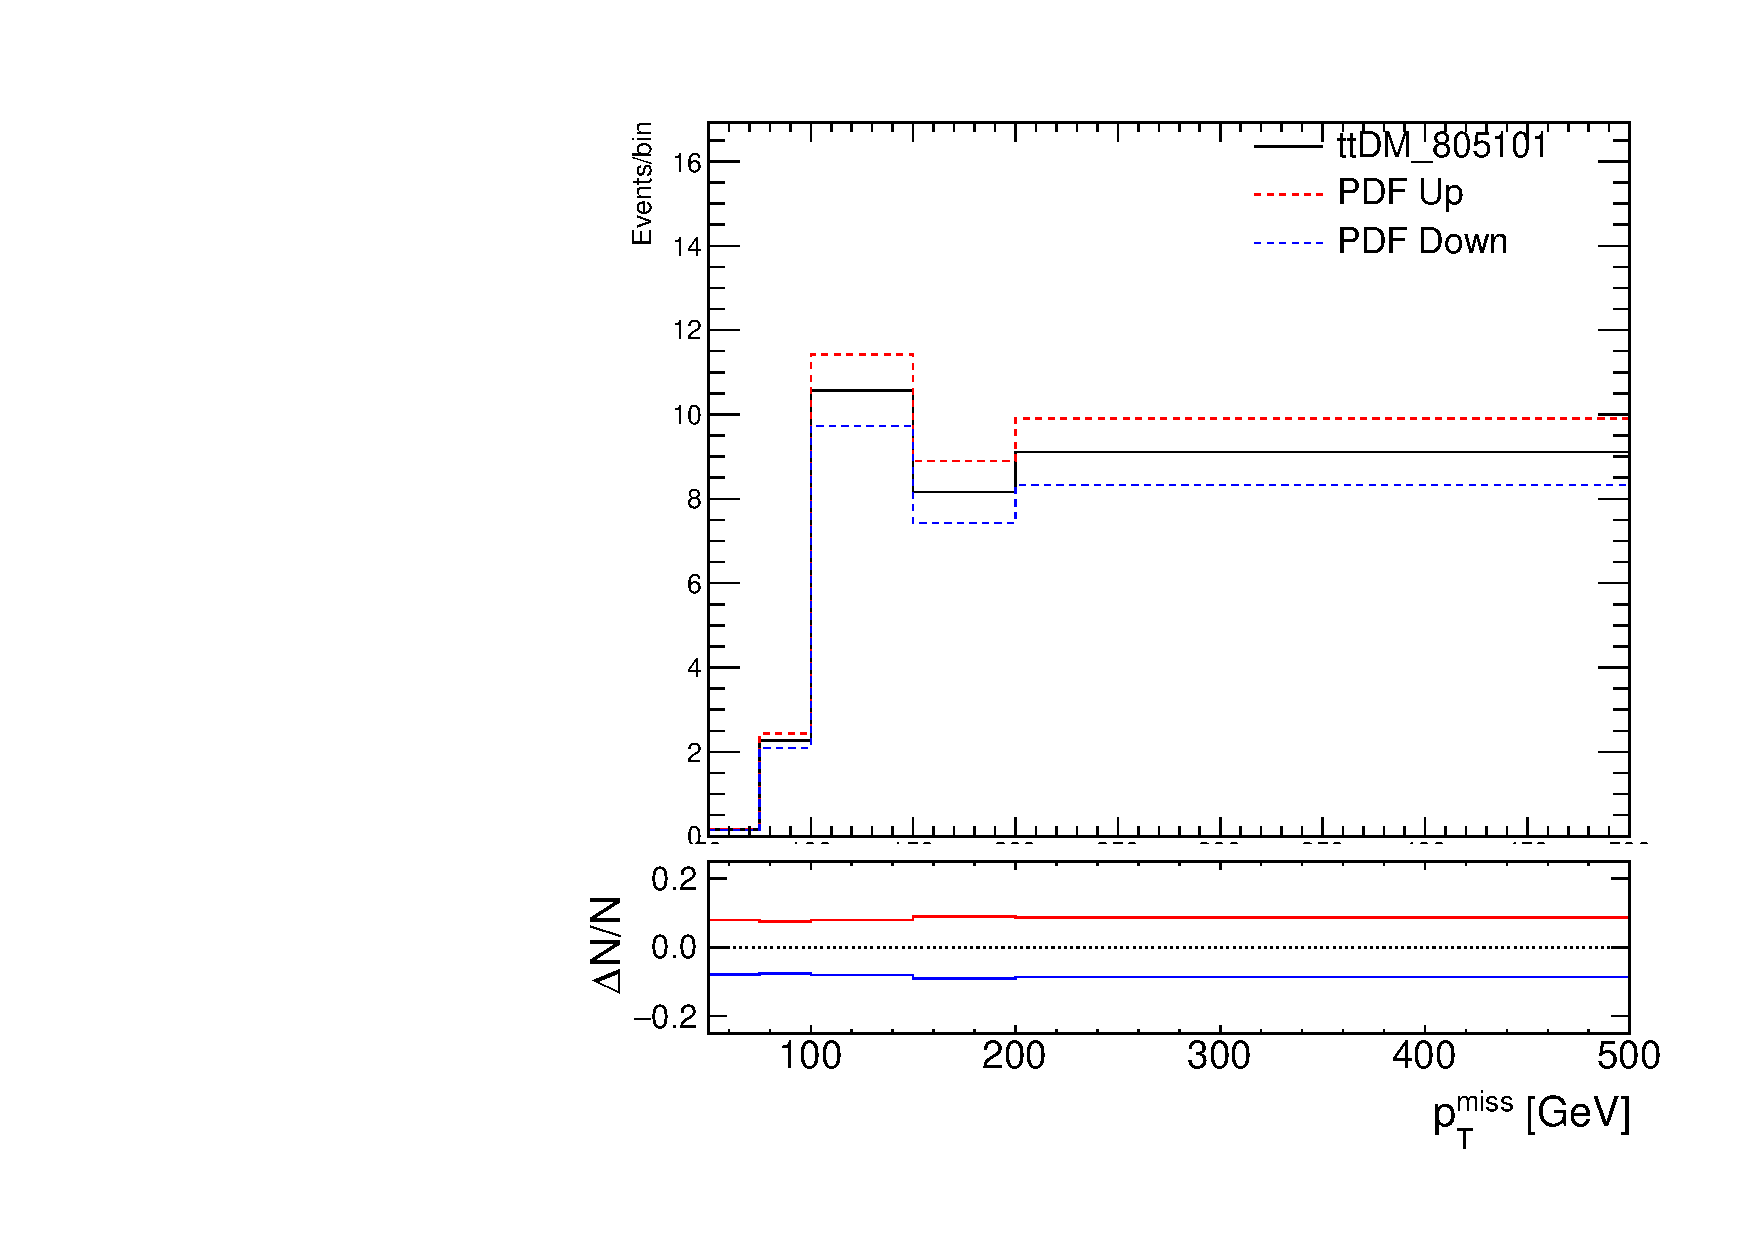
\includegraphics[width=0.48\textwidth]{systs/shapes_ttdm805101_em_hi/ttDM_805101_pdf}}
  \caption{The variation in the \ptmiss spectra for scalar mediated $\mMed=10\:\GeV$ signal with $\mDM=1\:\GeV$ in the low and high \mttll SRs due to the variation of the pdf uncertainty $+1\sigma$ (red) and $-1\sigma$ (blue). The normalized residuals of the ``up'' and ``down'' shapes are shown in the lower panel.}
  \label{fig:PDFshape}
\end{figure}

%% Big appendixes should be split off into separate files, just like chapters
%\input{app-myreallybigappendix}
